\documentclass[12pt]{book}
%\documentclass[aps,pre,onecolumn,superscriptaddress]{revtex4-1}
\usepackage{graphicx, epsfig,cancel}
\usepackage{color}
\usepackage{textcomp}
\usepackage{amssymb,amsmath,amsfonts} 
\usepackage{setspace}
\usepackage{hyperref}
% add the bibliography to the table of contents
\usepackage[nottoc,notlot,notlof]{tocbibind}
% for writing code snippets in latex
\usepackage{listings}
% use option disable to turn off all notes
\usepackage{todonotes}
\usepackage{bm}

\definecolor{dkgreen}{rgb}{0,0.6,0}
\definecolor{gray}{rgb}{0.5,0.5,0.5}
\definecolor{mauve}{rgb}{0.58,0,0.82}

\lstset{frame=tb,
  language=C++,
  aboveskip=3mm,
  belowskip=3mm,
  showstringspaces=false,
  columns=flexible,
  basicstyle={\small\ttfamily},
  numbers=none,
  numberstyle=\tiny\color{gray},
  keywordstyle=\color{blue},
  commentstyle=\color{dkgreen},
  stringstyle=\color{mauve},
  breaklines=true,
  breakatwhitespace=true,
  tabsize=3
}

\newcommand{\blue}[1]{\textcolor{blue}{#1}}
\newcommand{\red}[1]{\textcolor{red}{[#1]}}
\newcommand{\green}[1]{\textcolor{green}{#1}}

\usepackage{suffix}

\newcommand\chapterauthor[1]{\authortoc{#1}\printchapterauthor{#1}}
\WithSuffix\newcommand\chapterauthor*[1]{\printchapterauthor{#1}}

\makeatletter
\newcommand{\printchapterauthor}[1]{%
  {\parindent0pt\vspace*{-25pt}%
  \linespread{1.1}\large\scshape#1%
  \par\nobreak\vspace*{35pt}}
  \@afterheading%
}
\newcommand{\authortoc}[1]{%
  \addtocontents{toc}{\vskip-10pt}%
  \addtocontents{toc}{%
    \protect\contentsline{chapter}%
    {\hskip1.3em\mdseries\scshape\protect\scriptsize#1}{}{}}
  \addtocontents{toc}{\vskip5pt}%
}
\makeatother

\newcommand{\diff}{\mathop{}\!\mathrm{d}}
%\newcommand\numberthis{\addtocounter{equation}{1}\tag{\theequation}}
\renewcommand{\vec}[1]{\bm{#1}} % bolded regular vector
\newcommand{\mat}[1]{\bm{#1}} % matrix 
%\newcommand{\hvec}[1]{\ensuremath{\vec{\hat{#1}}}} % hat-vector
%\newcommand{\bvec}[1]{\ensuremath{\vec{\bar{#1}}}} % bar-vector 
%\newcommand{\sfnc}[1]{\ensuremath{\mathcal{#1}}} % scalar-valued function
%\newcommand{\vfnc}[1]{\ensuremath{\vec{\mathcal{#1}}}} % vector-valued function
%\newcommand{\rspc}[1]{\ensuremath{\mathbb{R}^{#1}}} % real vector space
%\newcommand{\pjac}[2]{\ensuremath{\; \frac{\partial #1}{\partial #2}} \;} % partial jacobian


%\includeonly{./Macroscale/Macroscale_Derivation,./Microscale/Microscale_Derivation,./Multiscale/MultiscaleNotes}
%\includeonly{./ConstitutiveRelationships/Constitutive}
%\includeonly{./VolumeConstrain/VolumeConstraint}

%\includeonly{./Multiscale/MultiscaleNotes}

\author{Victor Chan, Jacob Merson, Bill Tobin}
\title{Biotissue Reference Manual}

\begin{document}
\maketitle
\tableofcontents
\listoftodos

\part{Multiscale FEM Derivation}
\chapter{Macrocale Derivation}
\chapterauthor{V. W. L. Chan and W. R. Tobin}

\section{Motivation}

This chapter describes the formulation of the boundary value problem (BVP) at the macroscopic size scale. It discusses the weak form of the BVP, and solution method. It describes some of the numerical details which are needed to construct the macroscopic solution, e.g. the linear tetrahedral shape function, and residual formulation.

\section{Macro Scale}

\todo{replace with section \ref{sec:NLFEM}}
\subsection{Momentum Balance and Formulation of the Residual}

We are interested in solving the Cauchy Momentum Balance Equation for a body in static equilibrium and in absence of body forces:
%
\begin{align}
\nabla \cdot \pmb{\sigma} =& \; 0 \text{ in } \Omega \label{momentum_balance} \\
\pmb{\sigma} \cdot \pmb{n} =& \; \pmb{t} \text{ on } \partial \Omega \nonumber
\end{align}
%
where $\pmb{\Omega}$ is the problem domain, $\partial \pmb{\Omega}$ is the domain boundary, $\pmb{\sigma}$ is the Cauchy stress tensor, $\pmb{n}$ is the outward-facing unit normal along the domain boundary, and $\pmb{t}$ is the surface traction along the domain boundary.
%
\begin{eqnarray}
\pmb{\sigma} \equiv
\begin{bmatrix}
\sigma_{xx} & \sigma_{xy} & \sigma_{xz} \\
\sigma_{yx} & \sigma_{yy} & \sigma_{yz} \\
\sigma_{zx} & \sigma_{zy} & \sigma_{zz} 
\end{bmatrix} .
\label{cauchy_stress_tensor}
\end{eqnarray}
%

Since we intend to use the Galerkin Finite Element Method (FEM), we will need to consider the Galerkin weak form of Eq.\ \eqref{momentum_balance}. We obtain the weak or variational form of the equation by multiplying using an appropriate weighting function $\phi \in \pmb{V}$ where $\pmb{V}$ is an infinite-dimensional trial space and then integrating over the domain:

%
\begin{equation}
\int_\Omega \phi(\nabla \cdot \pmb{\sigma}) \diff \Omega = 0
\label{weak_form1}
\end{equation}
%

Using the divergence identity \todo{correct terminology?}

%
\begin{equation}
\nabla \cdot (\phi \pmb{\sigma}) = \pmb{\sigma} (\nabla \phi) + \phi (\nabla \cdot \pmb{\sigma}) \nonumber
\end{equation}
%

to arrive at 

%
\begin{equation}
\int_\Omega \nabla \cdot (\phi \pmb{\sigma}) - \pmb{\sigma} (\nabla \phi) \diff \Omega = 0
\label{weak_form2}
\end{equation}
%

separating the integrand terms and applying the Divergence Theorem to the first term we arrive at:

%
\begin{equation}
\int_{\partial \Omega} (\phi \pmb{\sigma}) \cdot \pmb{n} \; \diff \partial \Omega - \int_\Omega \pmb{\sigma} (\nabla \phi) \diff \Omega = 0
\label{weak_form3}
\end{equation}
%

where $\partial \Omega$ indicates that the integral is over the boundary of the domain and $\textbf{n}$ is the unit normal to the surface.

\todo[prepend, caption={Complete BVP derivation}]{I don't think we make this assumption in code formulation. E.G. we should show the formulation in terms of the full, BVP with no assumption.}
If we consider a surface-traction free problem, the first term in Eq.\ \eqref{weak_form3} goes to zero and we have

%
\begin{equation}
\int_\Omega \pmb{\sigma} \nabla \phi \diff \Omega = 0
\label{weak_form}
\end{equation}
%

Finally, we cast the problem in a Galerkin form by selecting a finite subspace of the trial space $\pmb{V}_h \subseteq \pmb{V}$ and selecting our trial functions from this finite subspace $\phi_i \in \pmb{V}_h$

%
\begin{equation}
\int_\Omega \pmb{\sigma} \nabla \phi_i \diff \Omega = 0
\label{galerkin_weak_form}
\end{equation}
%

which is the problem we will set out to solve in this note.

\todo{Should these matrices be explicitly written out, or can we just write them in summation form e.g. Hughes}
To clearly see the problem, the terms within the integral of Eq.\ \eqref{galerkin_weak_form} can be explicitly written out as
%
\begin{eqnarray}
\pmb{\sigma} \nabla \phi_i &=&
\begin{bmatrix}
\sigma_{xx} & \sigma_{xy} & \sigma_{xz} \\
\sigma_{yx} & \sigma_{yy} & \sigma_{yz} \\
\sigma_{zx} & \sigma_{zy} & \sigma_{zz} 
\end{bmatrix}
%
\begin{bmatrix}
\frac{\partial \phi_i}{\partial x} \\ \frac{\partial \phi_i}{\partial y} \\ \frac{\partial \phi_i}{\partial z}
\end{bmatrix} \nonumber\\
%
&=& 
%
\begin{bmatrix}
\sigma_{xx} \frac{\partial \phi_i}{\partial x} + \sigma_{xy} \frac{\partial \phi_i}{\partial y} + \sigma_{xz} \frac{\partial \phi_i}{\partial z} \\
%
\sigma_{yx} \frac{\partial \phi_i}{\partial x} + \sigma_{yy} \frac{\partial \phi_i}{\partial y} + \sigma_{yz} \frac{\partial \phi_i}{\partial z} \\
%
\sigma_{zx} \frac{\partial \phi_i}{\partial x} + \sigma_{zy} \frac{\partial \phi_i}{\partial y} + \sigma_{zz} \frac{\partial \phi_i}{\partial z} 
\end{bmatrix}
%
\end{eqnarray}
%
Therefore, Eq.\ \eqref{galerkin_weak_form} can be written as
%
\begin{eqnarray}
R_{ix} = \int_V \sigma_{xx} \frac{\partial \phi_i}{\partial x} + \sigma_{xy} \frac{\partial \phi_i}{\partial y} + \sigma_{xz} \frac{\partial \phi_i}{\partial z} dV \nonumber\\
%
R_{iy} = \int_V \sigma_{yx} \frac{\partial \phi_i}{\partial x} + \sigma_{yy} \frac{\partial \phi_i}{\partial y} + \sigma_{yz} \frac{\partial \phi_i}{\partial z} dV \nonumber\\
%
R_{iz} = \int_V \sigma_{zx} \frac{\partial \phi_i}{\partial x} + \sigma_{zy} \frac{\partial \phi_i}{\partial y} + \sigma_{zz} \frac{\partial \phi_i}{\partial z}  dV,
\label{residual_xyz}
\end{eqnarray}
%
where the $x$, $y$, and $z$ in the subscript indicate the $x$, $y$, and $z$ contributions to the residual, respectively.

\subsection{Newton-Raphson Procedure}

\todo[prepend, caption={NR wrong for specified BVP}]{this section makes no sense w.r.t the previous section. e.g. how are we solving a newton raphson iteration in displacements, when our bvp is formulated in terms of stresses and a weighting function.}
To minimize the residual in Eq.\ \eqref{galerkin_weak_form}, and hence solve the problem, the Newton-Raphson Procedure is used
%
\begin{equation}
\pmb{K}_T \delta u = -R, \ \ \text{where} \ \ u^{n+1} = u^{n} + \delta u,
\end{equation}
%

\todo[prepend,caption={incorrect residual}]{I think the residual should be in terms of the displacements, since the NR proceedure was written out in terms of displacements, granted you can make comment that taking derivative w.r.t. the current coord is same as taking the derivative w.r.t. the displacements.} and
%
\begin{eqnarray}
\pmb{K}_T \equiv
\begin{bmatrix}
\frac{\partial R_x}{\partial x_n} & \frac{\partial R_x}{\partial y_n} & \frac{\partial R_x}{\partial z_n} \\
\frac{\partial R_y}{\partial x_n} & \frac{\partial R_y}{\partial y_n} & \frac{\partial R_y}{\partial z_n} \\
\frac{\partial R_z}{\partial x_n} & \frac{\partial R_z}{\partial y_n} & \frac{\partial R_z}{\partial z_n} ,
\label{tangent_stiffness}
\end{bmatrix}
\end{eqnarray}
%

where $x_n$, $y_n$, and $z_n$ are the nodal positions (the vertices in this case) of the element.

As seen in Eq.\ \eqref{galerkin_weak_form} we are solving the problem at each node of the element. The derivatives indicated in Eq.\ \eqref{tangent_stiffness} for the $x$ contribution to each node are
%
\begin{eqnarray}
%%%%
\frac{\partial R_{ix}}{\partial x_n} &=& \frac{\partial R_{ix}}{\partial x_n} \bigg |_V + \frac{\partial R_{ix}}{\partial V} \frac{\partial V}{\partial x_n} \nonumber\\
&=& \int_V \left(\frac{\partial \sigma_{xx}}{\partial x_n}\frac{\partial \phi_i}{\partial x} + \frac{\partial \sigma_{xy}}{\partial x_n}\frac{\partial \phi_i}{\partial y} + \frac{\partial \sigma_{xz}}{\partial x_n}\frac{\partial \phi_i}{\partial z}  \right) dV \nonumber\\
&&+ \int_V \left( \sigma_{xx} \frac{\partial}{\partial x_n} \left(\frac{\partial \phi_i}{\partial x}\right)+\sigma_{xy} \frac{\partial}{\partial x_n} \left(\frac{\partial \phi_i}{\partial y}\right) + \sigma_{xz} \frac{\partial}{\partial x_n} \left(\frac{\partial \phi_i}{\partial z}\right) \right) dV \nonumber\\
&& + \left(  \sigma_{xx} \frac{\partial \phi_i}{\partial x} + \sigma_{xy} \frac{\partial \phi_i}{\partial y} + \sigma_{xz} \frac{\partial \phi_i}{\partial z} \right) \frac{\partial}{\partial x_n} \left(\int_V dV \right) \nonumber\\
%%%%
\frac{\partial R_{ix}}{\partial y_n} &=& \frac{\partial R_{ix}}{\partial y_n} \bigg |_V + \frac{\partial R_{ix}}{\partial V} \frac{\partial V}{\partial y_n} \nonumber\\
&=& \int_V \left(\frac{\partial \sigma_{xx}}{\partial y_n}\frac{\partial \phi_i}{\partial x} +\frac{\partial \sigma_{xy}}{\partial y_n}\frac{\partial \phi_i}{\partial y} +  \frac{\partial \sigma_{xz}}{\partial y_n}\frac{\partial \phi_i}{\partial z}  \right) dV \nonumber\\
&& + \int_V \left( \sigma_{xx} \frac{\partial}{\partial y_n} \left(\frac{\partial \phi_i}{\partial x}\right)+ \sigma_{xy} \frac{\partial}{\partial y_n} \left(\frac{\partial \phi_i}{\partial y}\right) + \sigma_{xz} \frac{\partial}{\partial y_n} \left(\frac{\partial \phi_i}{\partial z}\right) \right) dV \nonumber\\
&& + \left(  \sigma_{xx} \frac{\partial \phi_i}{\partial x} + \sigma_{xy} \frac{\partial \phi_i}{\partial y} + \sigma_{xz} \frac{\partial \phi_i}{\partial z} \right) \frac{\partial}{\partial y_n} \left(\int_V dV \right) \nonumber\\
%%%%
\frac{\partial R_{ix}}{\partial z_n} &=& \frac{\partial R_{ix}}{\partial z_n} \bigg |_V + \frac{\partial R_{ix}}{\partial V} \frac{\partial V}{\partial z_n} \nonumber\\
&=& \int_V \left(\frac{\partial \sigma_{xx}}{\partial z_n}\frac{\partial \phi_i}{\partial x} +\frac{\partial \sigma_{xy}}{\partial z_n} \frac{\partial \phi_i}{\partial y} + \frac{\partial \sigma_{xz}}{\partial z_n}\frac{\partial \phi_i}{\partial z}  \right) dV \nonumber\\
&&+ \int_V \left(\sigma_{xx} \frac{\partial}{\partial z_n} \left(\frac{\partial \phi_i}{\partial x}\right)+ \sigma_{xy} \frac{\partial}{\partial z_n} \left(\frac{\partial \phi_i}{\partial y}\right) + \sigma_{xz} \frac{\partial}{\partial z_n} \left(\frac{\partial \phi_i}{\partial z}\right) \right) dV \nonumber\\
&& + \left(  \sigma_{xx} \frac{\partial \phi_i}{\partial x} + \sigma_{xy} \frac{\partial \phi_i}{\partial y} + \sigma_{xz} \frac{\partial \phi_i}{\partial z} \right) \frac{\partial}{\partial z_n} \left(\int_V dV \right).
\label{dRx}
\end{eqnarray}
 \todo{write in indicial form, not sure if needed at all here, move to multiscale formulation section?}
%

Note that the derivatives of $R_{ix}$ takes into account the change in the residual due to the change in nodal position and due to the change in the volume of the element. Therefore, the changes in the residual due to change in volume but no change in stress state and due to change in stress state and no change in volume are both taken into account \red{this is essentially the 3D Leibniz integration rule. Discuss Eq.\ \eqref{dRx} in terms of Leibniz integration rule}. The derivatives of $R_{iy}$ and $R_{iz}$ are written out in the Appendix \ref{app:dRy_and_dRz}.

The $\sigma_{rs}$, $\partial \sigma_{rs}/\partial x_n$, $\partial \sigma_{rs}/\partial y_n$, and $\partial \sigma_{rs}/\partial z_n$ terms in Eq.\ \eqref{dRx} are determined from the micro scale calculations (see later section). In order to evaluate the $\partial \phi_i/\partial x$ and $\partial /\partial x_n (\partial \phi_i/\partial x)$ terms, we need to first specify the specific shape functions that are used for our calculations.\todo{We need to state that we can pull out the stresses due to the fact that they are just nodal constants.}

\subsection{Tetrahedral Shape Functions and Their Derivatives}
\todo{this section has not been edited yet.}
The shape functions, $\phi_i$, for the four nodes of a linear tetrahedral element are
%
\begin{equation}
\phi_1 = 1 - r - s - t, \ \ \phi_2 = r, \ \ \phi_3 = s, \ \ \text{and} \ \ \phi_4 = t,
\label{shape_fxns}
\end{equation}
%
where $(r,s,t)$ are the barycentric coordinates of a tetrahedron. The geometry of our problem $(x,y,z)$ can be written in terms of the shape functions, $\phi_i$, as
%
\begin{eqnarray}
x &=& \sum_{i}^4 x_i \phi_i = x_1 \phi_1 + x_2 \phi_2 + x_3 \phi_3 + x_4 \phi_4 \nonumber\\
y &=& \sum_i^4 y_i \phi_i =  y_1 \phi_1 + y_2 \phi_2 + y_3 \phi_3 + y_4 \phi_4  \nonumber\\
z &=& \sum_i^4  z_i \phi_i =  z_1 \phi_1 + z_2 \phi_2 + z_3 \phi_3 + z_4 \phi_4 ,
\label{geometry}
\end{eqnarray}
%
where $x_i$, $y_i$, and $z_i$ are the nodal positions (i.e., $x_i = x_n$, $y_i = y_n$, and $z_i = z_n$) of a tetrahedral element. As seen in Eq.\ \eqref{dRx}, we require the derivative of $\phi_i$ with respect to $x$, $y$, and $z$. In order to obtain such derivatives, we use the relationships
%
\begin{eqnarray}
%
\begin{bmatrix}
\frac{\partial \phi_i}{\partial r} \\
\frac{\partial \phi_i}{\partial s} \\
\frac{\partial \phi_i}{\partial t}
\end{bmatrix} &=&
%
J^T
%
\begin{bmatrix}
\frac{\partial \phi_i}{\partial x} \\
\frac{\partial \phi_i}{\partial y} \\
\frac{\partial \phi_i}{\partial z}
\end{bmatrix} \ \ \rightarrow \ \ 
%
%
\begin{bmatrix}
\frac{\partial \phi_i}{\partial x} \\
\frac{\partial \phi_i}{\partial y} \\
\frac{\partial \phi_i}{\partial z}
\end{bmatrix} =
%
(J^T)^{-1}
%
\begin{bmatrix}
\frac{\partial \phi_i}{\partial r} \\
\frac{\partial \phi_i}{\partial s} \\
\frac{\partial \phi_i}{\partial t}
\end{bmatrix}
\label{dx_to_dr}
\end{eqnarray}
%
where
%
\begin{eqnarray}
J^T &\equiv&
% 
\begin{bmatrix}
\frac{\partial x}{\partial r} & \frac{\partial y}{\partial r} & \frac{\partial z}{\partial r} \\
\frac{\partial x}{\partial s} & \frac{\partial y}{\partial s} & \frac{\partial z}{\partial s} \\
\frac{\partial x}{\partial t} & \frac{\partial y}{\partial t} & \frac{\partial z}{\partial t} 
\end{bmatrix} 
%
=
%
\begin{bmatrix}
\text{x}_1 & \text{y}_1 & \text{z}_1 \\
\text{x}_2 & \text{y}_2 & \text{z}_2 \\
\text{x}_3 & \text{y}_3 & \text{z}_3
\end{bmatrix} \ \ \text{and} \nonumber\\
%
(J^T)^{-1} &=& \frac{1}{\text{det}(J^T)} \begin{bmatrix}
\text{y}_2 \text{z}_3 - \text{y}_3 \text{z}_2 &-\text{y}_1 \text{z}_3 + \text{y}_3 \text{z}_1  & \text{y}_1 \text{z}_2 - \text{y}_2 \text{z}_1 \\
- \text{x}_2 \text{z}_3 + \text{x}_3\text{z}_2 & \text{x}_1\text{z}_3 - \text{x}_3 \text{z}_1 & -\text{x}_1 \text{z}_2 + \text{x}_2 \text{z}_1  \\
\text{x}_2 \text{y}_3 - \text{x}_3 \text{y}_2 & -\text{x}_1 \text{y}_3 + \text{x}_3 \text{y}_1 & \text{x}_1 \text{y}_2 - \text{x}_2 \text{y}_1
\end{bmatrix}.
\label{J}
\end{eqnarray}
%
The derivatives in $J^T$ can be straightforwardly determined by taking derivatives of Eq.\ \eqref{geometry} and using the definition of $\phi_i$ in Eq.\ \eqref{shape_fxns}. The derivatives are
%
\begin{eqnarray}
\text{x}_1 &=& \frac{\partial x}{\partial r} = -x_1 + x_2 , \ \ \
\text{y}_1 = \frac{\partial y}{\partial r} = -y_1 + y_2 , \ \ \
\text{z}_1 = \frac{\partial z}{\partial r} = -z_1 + z_2 \nonumber\\
%
\text{x}_2 &=& \frac{\partial x}{\partial s} = -x_1 + x_3 , \ \ \
\text{y}_2 = \frac{\partial y}{\partial s} = -y_1 + y_3, \ \ \  
\text{z}_2 = \frac{\partial z}{\partial s} = -z_1 + z_3 \nonumber\\
%
\text{x}_3 &=& \frac{\partial x}{\partial t} = - x_1 + x_4, \ \ \ 
\text{y}_3 = \frac{\partial y}{\partial t} = - y_1 + y_4, \ \ \ 
\text{z}_3 = \frac{\partial z}{\partial t} = -z_1 + z_4  \nonumber\\
%
\text{det}(J^T) &=& \text{x}_1 \left(\text{y}_2 \text{z}_3 - \text{z}_2\text{y}_3 \right) - \text{y}_1 \left(\text{x}_2 \text{z}_3 - \text{z}_2\text{x}_3 \right) + \text{z}_1 \left(\text{x}_2 \text{y}_3 - \text{y}_2\text{x}_3 \right).
\end{eqnarray}
%

Employing Eq.\ \eqref{dx_to_dr}, the derivatives of the shape functions with respect to $x$, $y$, and $z$ are
%
\begin{eqnarray}
%
\begin{bmatrix}
\frac{\partial \phi_i}{\partial x} \\
\frac{\partial \phi_i}{\partial y} \\
\frac{\partial \phi_i}{\partial z}
\end{bmatrix} = \frac{1}{\text{det}(J^T)}
%
\begin{bmatrix}
\left(\text{y}_2 \text{z}_3 - \text{y}_3 \text{z}_2\right) \frac{\partial \phi_i}{\partial r} + \left(-\text{y}_1 \text{z}_3 + \text{y}_3 \text{z}_1\right) \frac{\partial \phi_i}{\partial s} + \left(\text{y}_1 \text{z}_2 - \text{y}_2 \text{z}_1\right) \frac{\partial \phi_i}{\partial t} \\
%
\left(-\text{x}_2 \text{z}_3 + \text{x}_3\text{z}_2\right) \frac{\partial \phi_i}{\partial r} + \left(\text{x}_1\text{z}_3 - \text{x}_3 \text{z}_1\right) \frac{\partial \phi_i}{\partial s} + \left( -\text{x}_1 \text{z}_2 + \text{x}_2 \text{z}_1\right) \frac{\partial \phi_i}{\partial t} \\
%
\left(\text{x}_2 \text{y}_3 - \text{x}_3 \text{y}_2 \right) \frac{\partial \phi_i}{\partial r} + \left( -\text{x}_1 \text{y}_3 + \text{x}_3 \text{y}_1\right) \frac{\partial \phi_i}{\partial s} + \left( \text{x}_1 \text{y}_2 - \text{x}_2 \text{y}_1 \right) \frac{\partial \phi_i}{\partial t}
\end{bmatrix},
%
\end{eqnarray}
% 
%and are calculated in calc\_six\_dos.cc and stored as the variables ttkx, ttky, and ttkz.

As seen in Eq.\ \eqref{dRx}, we also need the derivatives of $\partial \phi_i/\partial x$, $\partial \phi_i/\partial y$, and $\partial \phi_i/\partial z$ terms with respect to $x_n$, $y_n$, and $y_n$ (the nodal positions). The derivatives of $\partial \phi_i/\partial x$, $\partial \phi_i/\partial y$, and $\partial \phi_i/\partial z$ with respect to $x_n$ are
%
\begin{eqnarray}
\frac{\partial}{\partial x_n} \left( \frac{\partial \phi_i}{\partial x} \right) &=&  -\frac{1}{(\text{det}(J^T))^2} \frac{\partial \text{det}(J^T)}{\partial x_n} P_x + \text{det}(J^T) \frac{\partial P_x}{\partial x_n}\nonumber\\
%%%%
\frac{\partial}{\partial y_n} \left( \frac{\partial \phi_i}{\partial x} \right) &=& -\frac{1}{(\text{det}(J^T))^2} \frac{\partial \text{det}(J^T)}{\partial y_n} P_x + \text{det}(J^T) \frac{\partial P_x}{\partial y_n} \nonumber\\
%%%%
\frac{\partial}{\partial z_n} \left( \frac{\partial \phi_i}{\partial x} \right) &=& -\frac{1}{(\text{det}(J^T))^2} \frac{\partial \text{det}(J^T)}{\partial z_n} P_x + \text{det}(J^T) \frac{\partial P_x}{\partial z_n} ,
\label{d2phi_dxdxn}
\end{eqnarray}
%
where $P_x$ is the first row of the dot product of the Adjoint matrix of $J^T$ with the gradient of the shape functions with respect to $r$, $s$, and $t$ and is explicitly represented as
%
\begin{equation}
P_x \equiv \left(\text{y}_2 \text{z}_3 - \text{y}_3 \text{z}_2\right) \frac{\partial \phi_i}{\partial r} + \left(-\text{y}_1 \text{z}_3 + \text{y}_3 \text{z}_1\right) \frac{\partial \phi_i}{\partial s} + \left(\text{y}_1 \text{z}_2 - \text{y}_2 \text{z}_1\right) \frac{\partial \phi_i}{\partial t}.
\label{Px}
\end{equation}
%

Similarly, the derivatives of $\partial \phi_i/\partial y$ and $\partial \phi_i/ \partial z$ are 
%
\begin{eqnarray}
\frac{\partial}{\partial x_n} \left( \frac{\partial \phi_i}{\partial y} \right) &=&  -\frac{1}{(\text{det}(J^T))^2} \frac{\partial \text{det}(J^T)}{\partial x_n} P_y + \text{det}(J^T) \frac{\partial P_y}{\partial x_n}\nonumber\\
%%%%
\frac{\partial}{\partial y_n} \left( \frac{\partial \phi_i}{\partial y} \right) &=& -\frac{1}{(\text{det}(J^T))^2} \frac{\partial \text{det}(J^T)}{\partial y_n} P_y + \text{det}(J^T) \frac{\partial P_y}{\partial y_n} \nonumber\\
%%%%
\frac{\partial}{\partial z_n} \left( \frac{\partial \phi_i}{\partial y} \right) &=& -\frac{1}{(\text{det}(J^T))^2} \frac{\partial \text{det}(J^T)}{\partial z_n} P_y + \text{det}(J^T) \frac{\partial P_y}{\partial z_n} 
\label{d2phi_dydxn}
\end{eqnarray}
%
and
%
\begin{eqnarray}
\frac{\partial}{\partial x_n} \left( \frac{\partial \phi_i}{\partial z} \right) &=&  -\frac{1}{(\text{det}(J^T))^2} \frac{\partial \text{det}(J^T)}{\partial x_n} P_z + \text{det}(J^T) \frac{\partial P_z}{\partial x_n}\nonumber\\
%%%%
\frac{\partial}{\partial y_n} \left( \frac{\partial \phi_i}{\partial z} \right) &=& -\frac{1}{(\text{det}(J^T))^2} \frac{\partial \text{det}(J^T)}{\partial y_n} P_z + \text{det}(J^T) \frac{\partial P_z}{\partial y_n} \nonumber\\
%%%%
\frac{\partial}{\partial z_n} \left( \frac{\partial \phi_i}{\partial z} \right) &=& -\frac{1}{(\text{det}(J^T))^2} \frac{\partial \text{det}(J^T)}{\partial z_n} P_z + \text{det}(J^T) \frac{\partial P_z}{\partial z_n} ,
\label{d2phi_dzdxn}
\end{eqnarray}
%
respectively, where $P_y$ and $P_z$ are the second and third row of the dot product of the Adjoint matrix of $J^T$ with the gradient of the shape functions with respect to $r$, $s$, and $t$. They are explicitly represented as
%
\begin{eqnarray}
P_y &\equiv& \left(-\text{x}_2 \text{z}_3 + \text{x}_3 \text{z}_2\right) \frac{\partial \phi_i}{\partial r} + \left(-\text{x}_1 \text{z}_3 - \text{x}_3 \text{z}_1\right) \frac{\partial \phi_i}{\partial s} + \left(-\text{x}_1 \text{z}_2 + \text{x}_2 \text{z}_1\right) \frac{\partial \phi_i}{\partial t} \nonumber\\
%
P_z &\equiv& \left(\text{x}_2 \text{y}_3 - \text{x}_3 \text{y}_2\right) \frac{\partial \phi_i}{\partial r} + \left(-\text{x}_1 \text{y}_3 + \text{x}_3 \text{y}_1\right) \frac{\partial \phi_i}{\partial s} + \left(\text{x}_1 \text{y}_2 - \text{x}_2 \text{y}_1\right) \frac{\partial \phi_i}{\partial t}.
%
\label{Py_and_Pz}
\end{eqnarray}
%
To determine the terms in Eqs.\ \eqref{d2phi_dxdxn}, \eqref{d2phi_dydxn}, and \eqref{d2phi_dzdxn} we need to explicitly write out the derivatives of det($J^T$), $P_x$, $P_y$, and $P_z$. 

\subsubsection{Derivative of det($J^T$) }

The derivative of det($J^T$) with respect to $x_n$ is
%
\begin{eqnarray}
\frac{\partial}{\partial x_n} \text{det}(J^T) &=& \text{det}
%
\begin{bmatrix}
\frac{\partial \text{x}_1}{\partial x_n} & \text{y}_1 & \text{z}_1 \\
\frac{\partial \text{x}_2}{\partial x_n} & \text{y}_2 & \text{z}_2 \\
\frac{\partial \text{x}_3}{\partial x_n} & \text{y}_3 & \text{z}_3
\end{bmatrix} \nonumber\\
%
&=& \frac{\partial \text{x}_1}{\partial x_n} \left(\text{y}_2 \text{z}_3 - \text{y}_3 \text{z}_2\right) - \text{y}_1 \left( \frac{\partial \text{x}_2}{\partial x_n} \text{z}_3 - \text{z}_2 \frac{\partial \text{x}_3}{\partial x_n} \right) + \text{z}_1 \left( \frac{\partial \text{x}_2}{\partial x_n} \text{y}_3 - \text{y}_2 \frac{\partial \text{x}_3}{\partial x_n} \right),
\end{eqnarray}
%
where
%
\begin{eqnarray}
\frac{\partial \text{x}_1}{\partial \text{x}_n} &=& \frac{\partial}{\partial x_n} \left( \frac{\partial x}{\partial r} \right) = \frac{\partial}{\partial x_n}\left(-x_1 + x_2 \right) = \frac{\partial \phi_n}{\partial r} \nonumber\\
%
\frac{\partial \text{x}_2}{\partial \text{x}_n} &=& \frac{\partial}{\partial x_n} \left( \frac{\partial x}{\partial s} \right) = \frac{\partial}{\partial x_n}\left(-x_1 + x_3  \right) = \frac{\partial \phi_n}{\partial s} \nonumber\\
%
\frac{\partial \text{x}_3}{\partial \text{x}_n} &=& \frac{\partial}{\partial x_n} \left( \frac{\partial x}{\partial t} \right) =  \frac{\partial}{\partial x_n}\left(-x_1+ x_4  \right) = \frac{\partial \phi_n}{\partial t}
%
\label{dxdxn_to_dphidr}
\end{eqnarray}
%
Therefore, we have
%
\begin{eqnarray}
%
\frac{\partial}{\partial x_n} \text{det}(J^T) &=&\text{det}
\begin{bmatrix}
\frac{\partial \phi_n}{\partial r} & \text{y}_1 & \text{z}_1 \\
\frac{\partial \phi_n}{\partial s} & \text{y}_2 & \text{z}_2 \\
\frac{\partial \phi_n}{\partial t} & \text{y}_3 & \text{z}_3
\end{bmatrix} \nonumber\\
%
&=& \frac{\partial \phi_n}{\partial r} \left(\text{y}_2 \text{z}_3 - \text{y}_3 \text{z}_2\right) - \text{y}_1 \left( \frac{\partial \phi_n}{\partial s} \text{z}_3 - \text{z}_2 \frac{\partial \phi_n}{\partial t} \right) + \text{z}_1 \left( \frac{\partial \phi_n}{\partial s} \text{y}_3 - \text{y}_2 \frac{\partial \phi_n}{\partial t} \right) 
\label{dJTx}
\end{eqnarray}
%
In Eq.\ \eqref{dJTx} the determinant is evaluated using a row expansion (expanded with respect to the first row). Interestingly, if we evaluate the determinant of the matrix using a column expansion (expanded with respect to the first column), we obtain the expression in Eq.\ \eqref{Px}. This suggests that, numerically, 
%
\begin{equation}
\frac{\partial}{\partial x_n} \text{det}(J^T) = P_x, \ \ \frac{\partial}{\partial y_n} \text{det}(J^T) = P_y, \ \ \text{and} \ \ \frac{\partial}{\partial z_n} \text{det}(J^T) = P_z,
\label{ddet_equal_P}
\end{equation}
%

where the derivatives of det($J^T$) with respect to $y_n$ and $z_n$ are derived similarly as above: 
%
\begin{eqnarray}
%
\frac{\partial}{\partial y_n} \text{det}(J^T) &=& \text{det}
%
\begin{bmatrix}
\text{x}_1 & \frac{\partial \text{y}_1}{\partial y_n} & \text{z}_1 \\
\text{x}_2 & \frac{\partial \text{y}_2}{\partial y_n} & \text{z}_2 \\
\text{x}_3 & \frac{\partial \text{y}_3}{\partial y_n} & \text{z}_3
\end{bmatrix} \nonumber\\
%
&=& x_1 \left(\frac{\partial \phi_n}{\partial s} \text{z}_3 - \frac{\partial \phi_n}{\partial t} \text{z}_2\right) - \frac{\partial \phi_n}{\partial r} \left(  \text{x}_2 \text{z}_3 - \text{z}_2 \text{x}_3 \right) + \text{z}_1 \left(  \text{x}_2 \frac{\partial \phi_n}{\partial t} - \frac{\partial \phi_n}{\partial s} \text{x}_3 \right) \nonumber\\
%%%%%%%
\frac{\partial}{\partial z_n} \text{det}(J^T) &=& \text{det}
%
\begin{bmatrix}
\text{x}_1 & \text{y}_1 & \frac{\partial \text{z}_1}{\partial z_n}  \\
\text{x}_2 & \text{y}_2 & \frac{\partial \text{z}_2}{\partial z_n}  \\
\text{x}_3 & \text{y}_3& \frac{\partial \text{z}_3}{\partial z_n}
\end{bmatrix} \nonumber\\
%
&=&  \text{x}_1 \left(\text{y}_2 \frac{\partial \phi_n}{\partial  t} - \text{y}_3 \frac{\partial \phi_n}{\partial s}\right) - \text{y}_1 \left( \text{x}_2 \frac{\partial \phi_n}{\partial t} - \frac{\partial \phi_n}{\partial s} \text{x}_3 \right) + \frac{\partial \phi_n}{\partial r} \left( \text{x}_2 \text{y}_3 - \text{y}_2 \text{x}_3 \right) . \nonumber\\
%
\label{dJT}
\end{eqnarray}

\subsubsection{Derivatives of $P_x$, $P_y$, and $P_z$}

The derivatives of $P_x$ are
%
\begin{eqnarray}
\frac{\partial P_x}{\partial x_n} &=& 0 \nonumber\\
%%%
\frac{\partial P_x}{\partial y_n} &=& \left(\frac{\partial \text{y}_2}{\partial y_n} \text{z}_3 - \frac{\partial\text{y}_3}{\partial y_n} \text{z}_2\right) \frac{\partial \phi_i}{\partial r} + \left(-\frac{\partial\text{y}_1}{\partial y_n} \text{z}_3 + \frac{\partial \text{y}_3}{\partial y_n} \text{z}_1\right) \frac{\partial \phi_i}{\partial s} + \left(\frac{\partial \text{y}_1}{\partial y_n} \text{z}_2 - \frac{\partial \text{y}_2}{\partial y_n} \text{z}_1\right) \frac{\partial \phi_i}{\partial t} \nonumber\\
%
&=& \left(\frac{\partial \phi_n}{\partial s} \text{z}_3 - \frac{\partial \phi_n}{\partial t} \text{z}_2\right) \frac{\partial \phi_i}{\partial r} + \left(-\frac{\partial\phi_n}{\partial r} \text{z}_3 + \frac{\partial \phi_n}{\partial t} \text{z}_1\right) \frac{\partial \phi_i}{\partial s} + \left(\frac{\partial \phi_n}{\partial r} \text{z}_2 - \frac{\partial \phi_n}{\partial s} \text{z}_1\right) \frac{\partial \phi_i}{\partial t} \nonumber\\
%
&=& \text{det}_{\text{col}} \begin{bmatrix}
\frac{\partial \phi_i}{\partial r} & \frac{\partial \phi_n}{\partial r} & z_1 \\
\frac{\partial \phi_i}{\partial s} & \frac{\partial \phi_n}{\partial s} & z_2 \\
\frac{\partial \phi_i}{\partial t} & \frac{\partial \phi_n}{\partial t} & z_3 
\end{bmatrix}\nonumber\\
%%%
\frac{\partial P_x}{\partial z_n} &=& \left(\text{y}_2 \frac{\partial \text{z}_3}{\partial z_n} - \text{y}_3 \frac{\partial \text{z}_2}{\partial z_n} \right) \frac{\partial \phi_i}{\partial r} + \left(-\text{y}_1 \frac{\partial\text{z}_3}{\partial z_n} + \text{y}_3 \frac{\partial\text{z}_1}{\partial z_n}\right) \frac{\partial \phi_i}{\partial s} + \left(\text{y}_1 \frac{\partial \text{z}_2}{\partial z_n} - \text{y}_2 \frac{\partial \text{z}_1}{\partial z_n}\right) \frac{\partial \phi_i}{\partial t}  \nonumber\\
%
 &=& \left(\text{y}_2 \frac{\partial \phi_n}{\partial t} - \text{y}_3 \frac{\partial \phi_n}{\partial s} \right) \frac{\partial \phi_i}{\partial r} + \left(-\text{y}_1 \frac{\partial\phi_n}{\partial t} + \text{y}_3 \frac{\partial\phi_n}{\partial r}\right) \frac{\partial \phi_i}{\partial s} + \left(\text{y}_1 \frac{\partial \phi_n}{\partial s} - \text{y}_2 \frac{\partial \phi_n}{\partial r}\right) \frac{\partial \phi_i}{\partial t}  \nonumber\\
 %
&=& \text{det}_{\text{col}} \begin{bmatrix}
\frac{\partial \phi_i}{\partial r} & y_1 & \frac{\partial \phi_n}{\partial r}  \\
\frac{\partial \phi_i}{\partial s} & y_2 & \frac{\partial \phi_n}{\partial s} \\
\frac{\partial \phi_i}{\partial t} & y_3 & \frac{\partial \phi_n}{\partial t}  
\end{bmatrix} ,
%
\label{dPx}
\end{eqnarray}
%
where we have used the relationships of the type in Eq.\ \eqref{dxdxn_to_dphidr} for the second equalities for $\partial P_x/\partial y_n$ and $\partial P_x/ \partial z_n$. The subscript ``col" indicates that the determinants are evaluated using a column expansion. Notice that shape functions with subscripts $i$ and $n$ are involved. The subscript $n$ corresponds to the ``current" node, while the subscript $i$ corresponds to the ``other" nodes in the element (including the current node).

The subscript ``col" is specified to ensure the correct analytical expression. Numerically, the determinant of the matrix is the same regardless of whether a row or column expansion is used. Following the pattern in Eq.\ \eqref{dPx}, the derivatives of $P_y$ and $P_z$ are 
%
\begin{eqnarray}
\frac{\partial P_y}{\partial x_n} &=&
\text{det} \begin{bmatrix}
\frac{\partial \phi_n}{\partial r} & \frac{\partial \phi_i}{\partial r} & z_1 \\
\frac{\partial \phi_n}{\partial s} & \frac{\partial \phi_i}{\partial s} & z_2 \\
\frac{\partial \phi_n}{\partial t} & \frac{\partial \phi_i}{\partial t} & z_3 
\end{bmatrix}, \ \ 
%
\frac{\partial P_y}{\partial y_n} = 0, \ \ 
%
\frac{\partial P_y}{\partial z_n} =
\text{det} \begin{bmatrix}
x_1 & \frac{\partial \phi_i}{\partial r} & \frac{\partial \phi_n}{\partial r} \\
x_2 & \frac{\partial \phi_i}{\partial s} & \frac{\partial \phi_n}{\partial s} \\
x_3 & \frac{\partial \phi_i}{\partial t} & \frac{\partial \phi_n}{\partial t} 
\end{bmatrix} \nonumber\\
%%%%%
\frac{\partial P_z}{\partial x_n} &=&
\text{det} \begin{bmatrix}
\frac{\partial \phi_n}{\partial r} & y_1 & \frac{\partial \phi_i}{\partial r}  \\
\frac{\partial \phi_n}{\partial s} & y_2 & \frac{\partial \phi_i}{\partial s} \\
\frac{\partial \phi_n}{\partial t} & y_3 & \frac{\partial \phi_i}{\partial t}  
\end{bmatrix}, \ \
%
\frac{\partial P_z}{\partial y_n} =
\text{det} \begin{bmatrix}
x_1 & \frac{\partial \phi_n}{\partial r} &  \frac{\partial \phi_i}{\partial r}  \\
x_2 & \frac{\partial \phi_n}{\partial s} &  \frac{\partial \phi_i}{\partial s} \\
x_3 & \frac{\partial \phi_n}{\partial t} &  \frac{\partial \phi_i}{\partial t}  
\end{bmatrix}, \ \
%
\frac{\partial P_z}{\partial y_n} = 0 .
\label{dPy_and_dPz}
\end{eqnarray}
% 

\subsubsection{Combining It All Together}

Substituting the relationships in Eqs.\ \eqref{dJTx}, \eqref{ddet_equal_P}, and \eqref{dPx} into Eq.\ \eqref{d2phi_dxdxn} we have
%
\begin{eqnarray}
\frac{\partial}{\partial x_n} \left( \frac{\partial \phi_i}{\partial x} \right) &=&  -\frac{P_x^2}{(\text{det}(J^T))^2}  \nonumber\\
%%%%%
\frac{\partial}{\partial y_n} \left( \frac{\partial \phi_i}{\partial x} \right) &=& -\frac{P_y P_x}{(\text{det}(J^T))^2} + \text{det}(J^T) \text{det}_{\text{col}} \begin{bmatrix}
\frac{\partial \phi_i}{\partial r} & \frac{\partial \phi_n}{\partial r} & z_1 \\
\frac{\partial \phi_i}{\partial s} & \frac{\partial \phi_n}{\partial s} & z_2 \\
\frac{\partial \phi_i}{\partial t} & \frac{\partial \phi_n}{\partial t} & z_3 
\end{bmatrix} \nonumber\\
%%%%%
\frac{\partial}{\partial z_n} \left( \frac{\partial \phi_i}{\partial x} \right) &=& -\frac{P_z P_x}{(\text{det}(J^T))^2} + \text{det}(J^T) \text{det}_{\text{col}} \begin{bmatrix}
\frac{\partial \phi_i}{\partial r} & y_1 & \frac{\partial \phi_n}{\partial r}  \\
\frac{\partial \phi_i}{\partial s} & y_2 & \frac{\partial \phi_n}{\partial s} \\
\frac{\partial \phi_i}{\partial t} & y_3 & \frac{\partial \phi_n}{\partial t}  
\end{bmatrix} .
\label{dkdx}
\end{eqnarray}
%

Similarly, substituting the relationships in Eqs.\ \eqref{dJT}, \eqref{ddet_equal_P}, and \eqref{dPy_and_dPz} in Eqs.\ \eqref{d2phi_dydxn} and \eqref{d2phi_dzdxn} we have
%
\begin{eqnarray}
\frac{\partial}{\partial x_n} \left( \frac{\partial \phi_i}{\partial y} \right) &=&  -\frac{P_x P_y}{(\text{det}(J^T))^2} + \text{det}(J^T) \text{det} \begin{bmatrix}
\frac{\partial \phi_n}{\partial r} & \frac{\partial \phi_i}{\partial r} & z_1 \\
\frac{\partial \phi_n}{\partial s} & \frac{\partial \phi_i}{\partial s} & z_2 \\
\frac{\partial \phi_n}{\partial t} & \frac{\partial \phi_i}{\partial t} & z_3 
\end{bmatrix} \nonumber\\
%%%%%
\frac{\partial}{\partial y_n} \left( \frac{\partial \phi_i}{\partial y} \right) &=& -\frac{P_y^2}{(\text{det}(J^T))^2}  \nonumber\\
%%%%%
\frac{\partial}{\partial z_n} \left( \frac{\partial \phi_i}{\partial y} \right) &=& -\frac{P_z P_y}{(\text{det}(J^T))^2} + \text{det}(J^T) \text{det} \begin{bmatrix}
x_1 & \frac{\partial \phi_i}{\partial r} & \frac{\partial \phi_n}{\partial r} \\
x_2 & \frac{\partial \phi_i}{\partial s} & \frac{\partial \phi_n}{\partial s} \\
x_3 & \frac{\partial \phi_i}{\partial t} & \frac{\partial \phi_n}{\partial t} 
\end{bmatrix} 
\label{dkdy}
\end{eqnarray}
%
and
%
\begin{eqnarray}
\frac{\partial}{\partial x_n} \left( \frac{\partial \phi_i}{\partial z} \right) &=&  -\frac{P_x P_z}{(\text{det}(J^T))^2} + \text{det}(J^T) \text{det} \begin{bmatrix}
\frac{\partial \phi_n}{\partial r} & y_1 & \frac{\partial \phi_i}{\partial r}  \\
\frac{\partial \phi_n}{\partial s} & y_2 & \frac{\partial \phi_i}{\partial s} \\
\frac{\partial \phi_n}{\partial t} & y_3 & \frac{\partial \phi_i}{\partial t}  
\end{bmatrix} \nonumber\\
%%%%%
\frac{\partial}{\partial y_n} \left( \frac{\partial \phi_i}{\partial y} \right) &=& -\frac{P_y P_z}{(\text{det}(J^T))^2} + \text{det}(J^T)\text{det} \begin{bmatrix}
x_1 & \frac{\partial \phi_n}{\partial r} &  \frac{\partial \phi_i}{\partial r}  \\
x_2 & \frac{\partial \phi_n}{\partial s} &  \frac{\partial \phi_i}{\partial s} \\
x_3 & \frac{\partial \phi_n}{\partial t} &  \frac{\partial \phi_i}{\partial t}  
\end{bmatrix} \nonumber\\
%%%%%
\frac{\partial}{\partial z_n} \left( \frac{\partial \phi_i}{\partial y} \right) &=& -\frac{P_z^2 }{(\text{det}(J^T))^2} .
\label{dkdz}
\end{eqnarray}
%
The above terms are calculated in microscale. % and the derivatives of $\partial \phi_i/\partial x$ with respect to $x_n$, $y_n$, and $z_n$ are stored in the variable dkdx as dkdx[in][3*n], dkdx[in][3*n+1], and dkdx[in][3*n+2], respectively. Note that ``in" corresponds to the subscript $n$, while ``n'' corresponds to the subscript $i$. Since we are employing a linear tetrahedral element, ``in" and ``n" range from 0 to 3. 

Each node of the tetrahedral element contains three derivatives $(\partial/\partial x_n, \partial/\partial y_n, \partial/\partial z_n)$ for each shape function (total of 4 for the tetrahedral element). Therefore, each node contains 12 entries. Since there are 4 nodes for each tetrahedral element, dkdx for each element is a 4 $\times$ 12 array:
%
\begin{eqnarray}
dkdx = 
%
\begin{bmatrix}
\frac{\partial}{\partial x_1}\left(\frac{\partial \phi_1}{\partial x}\right) & \frac{\partial}{\partial y_1}\left(\frac{\partial \phi_1}{\partial x}\right) & \frac{\partial}{\partial z_1}\left(\frac{\partial \phi_1}{\partial x}\right) & \cdots &\frac{\partial}{\partial x_1}\left(\frac{\partial \phi_4}{\partial x}\right) & \frac{\partial}{\partial y_1}\left(\frac{\partial \phi_4}{\partial x}\right) & \frac{\partial}{\partial z_1}\left(\frac{\partial \phi_4}{\partial x}\right) \\
%%
\frac{\partial}{\partial x_2}\left(\frac{\partial \phi_1}{\partial x}\right) & \frac{\partial}{\partial y_2}\left(\frac{\partial \phi_1}{\partial x}\right) & \frac{\partial}{\partial z_2}\left(\frac{\partial \phi_1}{\partial x}\right) & \cdots &\frac{\partial}{\partial x_2}\left(\frac{\partial \phi_4}{\partial x}\right) & \frac{\partial}{\partial y_2}\left(\frac{\partial \phi_4}{\partial x}\right) & \frac{\partial}{\partial z_2}\left(\frac{\partial \phi_4}{\partial x}\right) \\
%%
\frac{\partial}{\partial x_3}\left(\frac{\partial \phi_1}{\partial x}\right) & \frac{\partial}{\partial y_3}\left(\frac{\partial \phi_1}{\partial x}\right) & \frac{\partial}{\partial z_3}\left(\frac{\partial \phi_1}{\partial x}\right) & \cdots &\frac{\partial}{\partial x_3}\left(\frac{\partial \phi_4}{\partial x}\right) & \frac{\partial}{\partial y_3}\left(\frac{\partial \phi_4}{\partial x}\right) & \frac{\partial}{\partial z_3}\left(\frac{\partial \phi_4}{\partial x}\right) \\
%%
\frac{\partial}{\partial x_4}\left(\frac{\partial \phi_1}{\partial x}\right) & \frac{\partial}{\partial y_4}\left(\frac{\partial \phi_1}{\partial x}\right) & \frac{\partial}{\partial z_4}\left(\frac{\partial \phi_1}{\partial x}\right) & \cdots & \frac{\partial}{\partial x_4}\left(\frac{\partial \phi_4}{\partial x}\right) & \frac{\partial}{\partial y_4}\left(\frac{\partial \phi_4}{\partial x}\right) & \frac{\partial}{\partial z_4}\left(\frac{\partial \phi_4}{\partial x}\right)
\end{bmatrix},
\end{eqnarray}
%
where the rows correspond to the ``current" node number and the columns correspond to the derivative of the shape functions of the ``other" nodes with respect to $x_n$, $y_n$, and $z_n$.

The derivatives of $\partial \phi_i/\partial y$ and $\partial \phi_i/\partial z$ with respect to $x_n$, $y_n$, and $z_n$ are determined by following the same procedures used to determine the derivatives in Eq.\ \eqref{dkdx}. These terms, dkdy and dkdz, are explicitly written out in the appendix \todo{need to add this later}.

\section{Code Implementation of Macro Scale}

We need to create a 12 $\times$ 12 elemental tangent stiffness matrix, $K_e$, for each element that is formed from the derivatives of the residual:
%
\setcounter{MaxMatrixCols}{12}
\begin{eqnarray}
K_e = 
\begin{bmatrix}
\frac{\partial R_{1x}}{\partial x_1} & \frac{\partial R_{1x}}{\partial y_1} & \frac{\partial R_{1x}}{\partial z_1} & \frac{\partial R_{2x}}{\partial x_1} & \frac{\partial R_{2x}}{\partial y_1} & \frac{\partial R_{2x}}{\partial z_1} & \frac{\partial R_{3x}}{\partial x_1} & \frac{\partial R_{3x}}{\partial y_1} & \frac{\partial R_{3x}}{\partial z_1} & \frac{\partial R_{4x}}{\partial x_1} & \frac{\partial R_{4x}}{\partial y_1} & \frac{\partial R_{4x}}{\partial z_1} \\
%%%%%
\frac{\partial R_{1y}}{\partial x_1} & \frac{\partial R_{1y}}{\partial y_1} & \frac{\partial R_{1y}}{\partial z_1} & \frac{\partial R_{2y}}{\partial x_1} & \frac{\partial R_{2y}}{\partial y_1} & \frac{\partial R_{2y}}{\partial z_1} & \frac{\partial R_{3y}}{\partial x_1} & \frac{\partial R_{3y}}{\partial y_1} & \frac{\partial R_{3y}}{\partial z_1} & \frac{\partial R_{4y}}{\partial x_1} & \frac{\partial R_{4y}}{\partial y_1} & \frac{\partial R_{4y}}{\partial z_1} \\
%%%%%
\frac{\partial R_{1z}}{\partial x_1} & \frac{\partial R_{1z}}{\partial y_1} & \frac{\partial R_{1z}}{\partial z_1} & \frac{\partial R_{2z}}{\partial x_1} & \frac{\partial R_{2z}}{\partial y_1} & \frac{\partial R_{2z}}{\partial z_1} & \frac{\partial R_{3z}}{\partial x_1} & \frac{\partial R_{3z}}{\partial y_1} & \frac{\partial R_{3z}}{\partial z_1} & \frac{\partial R_{4z}}{\partial x_1} & \frac{\partial R_{4z}}{\partial y_1} & \frac{\partial R_{4z}}{\partial z_1} \\
%%%%%%
%%%%%%
%%%%%%
\frac{\partial R_{1x}}{\partial x_2} & \frac{\partial R_{1x}}{\partial y_2} & \frac{\partial R_{1x}}{\partial z_2} & \frac{\partial R_{2x}}{\partial x_2} & \frac{\partial R_{2x}}{\partial y_2} & \frac{\partial R_{2x}}{\partial z_2} & \frac{\partial R_{3x}}{\partial x_2} & \frac{\partial R_{3x}}{\partial y_2} & \frac{\partial R_{3x}}{\partial z_2} & \frac{\partial R_{4x}}{\partial x_2} & \frac{\partial R_{4x}}{\partial y_2} & \frac{\partial R_{4x}}{\partial z_2} \\
%%%%%
\frac{\partial R_{1y}}{\partial x_2} & \frac{\partial R_{1y}}{\partial y_2} & \frac{\partial R_{1y}}{\partial z_2} & \frac{\partial R_{2y}}{\partial x_2} & \frac{\partial R_{2y}}{\partial y_2} & \frac{\partial R_{2y}}{\partial z_2} & \frac{\partial R_{3y}}{\partial x_2} & \frac{\partial R_{3y}}{\partial y_2} & \frac{\partial R_{3y}}{\partial z_2} & \frac{\partial R_{4y}}{\partial x_2} & \frac{\partial R_{4y}}{\partial y_2} & \frac{\partial R_{4y}}{\partial z_2} \\
%%%%%
\frac{\partial R_{1z}}{\partial x_2} & \frac{\partial R_{1z}}{\partial y_2} & \frac{\partial R_{1z}}{\partial z_2} & \frac{\partial R_{2z}}{\partial x_2} & \frac{\partial R_{2z}}{\partial y_2} & \frac{\partial R_{2z}}{\partial z_2} & \frac{\partial R_{3z}}{\partial x_2} & \frac{\partial R_{3z}}{\partial y_2} & \frac{\partial R_{3z}}{\partial z_2} & \frac{\partial R_{4z}}{\partial x_2} & \frac{\partial R_{4z}}{\partial y_2} & \frac{\partial R_{4z}}{\partial z_2} \\
%%%%%%
%%%%%%
%%%%%%
\frac{\partial R_{1x}}{\partial x_3} & \frac{\partial R_{1x}}{\partial y_3} & \frac{\partial R_{1x}}{\partial z_3} & \frac{\partial R_{2x}}{\partial x_3} & \frac{\partial R_{2x}}{\partial y_3} & \frac{\partial R_{2x}}{\partial z_3} & \frac{\partial R_{3x}}{\partial x_3} & \frac{\partial R_{3x}}{\partial y_3} & \frac{\partial R_{3x}}{\partial z_3} & \frac{\partial R_{4x}}{\partial x_3} & \frac{\partial R_{4x}}{\partial y_3} & \frac{\partial R_{4x}}{\partial z_3} \\
%%%%%
\frac{\partial R_{1y}}{\partial x_3} & \frac{\partial R_{1y}}{\partial y_3} & \frac{\partial R_{1y}}{\partial z_3} & \frac{\partial R_{2y}}{\partial x_3} & \frac{\partial R_{2y}}{\partial y_3} & \frac{\partial R_{2y}}{\partial z_3} & \frac{\partial R_{3y}}{\partial x_3} & \frac{\partial R_{3y}}{\partial y_3} & \frac{\partial R_{3y}}{\partial z_3} & \frac{\partial R_{4y}}{\partial x_3} & \frac{\partial R_{4y}}{\partial y_3} & \frac{\partial R_{4y}}{\partial z_3} \\
%%%%%
\frac{\partial R_{1z}}{\partial x_3} & \frac{\partial R_{1z}}{\partial y_3} & \frac{\partial R_{1z}}{\partial z_3} & \frac{\partial R_{2z}}{\partial x_3} & \frac{\partial R_{2z}}{\partial y_3} & \frac{\partial R_{2z}}{\partial z_3} & \frac{\partial R_{3z}}{\partial x_3} & \frac{\partial R_{3z}}{\partial y_3} & \frac{\partial R_{3z}}{\partial z_3} & \frac{\partial R_{4z}}{\partial x_3} & \frac{\partial R_{4z}}{\partial y_3} & \frac{\partial R_{4z}}{\partial z_3} \\
%%%%%%
%%%%%%
%%%%%%
\frac{\partial R_{1x}}{\partial x_4} & \frac{\partial R_{1x}}{\partial y_4} & \frac{\partial R_{1x}}{\partial z_4} & \frac{\partial R_{2x}}{\partial x_4} & \frac{\partial R_{2x}}{\partial y_4} & \frac{\partial R_{2x}}{\partial z_4} & \frac{\partial R_{3x}}{\partial x_4} & \frac{\partial R_{3x}}{\partial y_4} & \frac{\partial R_{3x}}{\partial z_4} & \frac{\partial R_{4x}}{\partial x_4} & \frac{\partial R_{4x}}{\partial y_4} & \frac{\partial R_{4x}}{\partial z_4} \\
%%%%%
\frac{\partial R_{1y}}{\partial x_4} & \frac{\partial R_{1y}}{\partial y_4} & \frac{\partial R_{1y}}{\partial z_4} & \frac{\partial R_{2y}}{\partial x_4} & \frac{\partial R_{2y}}{\partial y_4} & \frac{\partial R_{2y}}{\partial z_4} & \frac{\partial R_{3y}}{\partial x_4} & \frac{\partial R_{3y}}{\partial y_4} & \frac{\partial R_{3y}}{\partial z_4} & \frac{\partial R_{4y}}{\partial x_4} & \frac{\partial R_{4y}}{\partial y_4} & \frac{\partial R_{4y}}{\partial z_4} \\
%%%%%
\frac{\partial R_{1z}}{\partial x_4} & \frac{\partial R_{1z}}{\partial y_4} & \frac{\partial R_{1z}}{\partial z_4} & \frac{\partial R_{2z}}{\partial x_4} & \frac{\partial R_{2z}}{\partial y_4} & \frac{\partial R_{2z}}{\partial z_4} & \frac{\partial R_{3z}}{\partial x_4} & \frac{\partial R_{3z}}{\partial y_4} & \frac{\partial R_{3z}}{\partial z_4} & \frac{\partial R_{4z}}{\partial x_4} & \frac{\partial R_{4z}}{\partial y_4} & \frac{\partial R_{4z}}{\partial z_4} \\
\end{bmatrix}
\end{eqnarray}
%

\subsection{First Term}

Each node of an element contains 9 terms: three terms each for the $x_n$ (see Eq.\ \eqref{dRx}), $y_n$, and $z_n$ contributions. 

The code snippet:
%
\begin{lstlisting}
apf::DynamicMatrix stress_derivs(9,9);                                                                                                                                                                            
apf::DynamicMatrix shape_grads(3,9);
for(int ii = 0; ii < nenodes; ii++)
	{
	// determine "force" vector.
	for (int jj = 0; jj < nenodes; jj++)
		{
		// extract j1, j2, and j3.
		for(int kk = 0; kk < 3; kk++)
			{
            		shape_grads(0,kk) = grads[ii][kk];
            		shape_grads(1,3+kk) = grads[ii][kk];
            		shape_grads(2,6+kk) = grads[ii][kk];
            		for(int ll = 0; ll < 3; ll++)
            			{
              	 		stress_derivs(kk,ll) = j1[kk][ll];
              	 		stress_derivs(3+kk,3+ll) = j2[kk][ll];
              	 		stress_derivs(6+kk,6+ll) = j3[kk][ll];
            			}
          		} // end loop for ll
		} // end loop for jj
	} // end loop for ii
\end{lstlisting}
%
produces the following matrices
%
\begin{eqnarray}
\text{shape\_grads} &=& 
\begin{bmatrix}
\frac{\partial \phi_i}{\partial x} & \frac{\partial \phi_i}{\partial y} & \frac{\partial \phi_i}{\partial z} & 0 & 0 & 0 & 0 & 0 & 0 \\
0 & 0 & 0 & \frac{\partial \phi_i}{\partial x} & \frac{\partial \phi_i}{\partial y} & \frac{\partial \phi_i}{\partial z} & 0 & 0 & 0 \\
0 & 0 & 0 & 0 & 0 & 0 & \frac{\partial \phi_i}{\partial x} & \frac{\partial \phi_i}{\partial y} & \frac{\partial \phi_i}{\partial z} 
\end{bmatrix} \ \ \text{and} \nonumber\\
%
\text{stress\_derivs} &=&
\begin{bmatrix}
\frac{\partial \sigma_{xx}}{\partial x_n} & \frac{\partial \sigma_{xy}}{\partial x_n} & \frac{\partial \sigma_{xz}} {\partial x_n} & 0 & 0 & 0 & 0 & 0 & 0 \\
%
\frac{\partial \sigma_{yx}}{\partial x_n} & \frac{\partial \sigma_{yy}}{\partial x_n} & \frac{\partial \sigma_{yz}} {\partial x_n} & 0 & 0 & 0 & 0 & 0 & 0 \\
%
\frac{\partial \sigma_{zx}}{\partial x_n} & \frac{\partial \sigma_{zy}}{\partial x_n} & \frac{\partial \sigma_{zz}} {\partial x_n} & 0 & 0 & 0 & 0 & 0 & 0 \\
%%%%
0 & 0 & 0 & \frac{\partial \sigma_{xx}}{\partial y_n} & \frac{\partial \sigma_{xy}}{\partial y_n} & \frac{\partial \sigma_{xz}} {\partial y_n} &  0 & 0 & 0 \\
%
0 & 0 & 0 & \frac{\partial \sigma_{yx}}{\partial y_n} & \frac{\partial \sigma_{yy}}{\partial y_n} & \frac{\partial \sigma_{yz}} {\partial y_n} &  0 & 0 & 0 \\
%
0 & 0 & 0 & \frac{\partial \sigma_{zx}}{\partial y_n} & \frac{\partial \sigma_{zy}}{\partial y_n} & \frac{\partial \sigma_{zz}} {\partial y_n} &  0 & 0 & 0 \\
%%%%
0 & 0 & 0 &  0 & 0 & 0 & \frac{\partial \sigma_{xx}}{\partial z_n} & \frac{\partial \sigma_{xy}}{\partial z_n} & \frac{\partial \sigma_{xz}} {\partial z_n}  \\
%
0 & 0 & 0 &  0 & 0 & 0 & \frac{\partial \sigma_{yx}}{\partial z_n} & \frac{\partial \sigma_{yy}}{\partial z_n} & \frac{\partial \sigma_{yz}} {\partial z_n}  \\
%
0 & 0 & 0 &  0 & 0 & 0 & \frac{\partial \sigma_{zx}}{\partial z_n} & \frac{\partial \sigma_{zy}}{\partial z_n} & \frac{\partial \sigma_{zz}} {\partial z_n}  
\end{bmatrix}.
\end{eqnarray}
%
Note that the subscript $i$ in shape\_grads corresponds to the $i^{th}$ shape function. A linear tetrahedral element is described by 4 shape functions, which are written out in Eq.\ \eqref{shape_fxns}. The subscript $i$ is represented by the variable ii in the code snippet above. Since the derivative of each shape function can be taken with respect to either $x$, $y$, or $z$, the shape\_grads array contains three unique derivatives for each shape function. The derivatives with respect to $x$, $y$, and $z$ are denoted by kk=0, 1, and 2, respectively, as seen in the code snippet above.   

Also note that the stress derivatives in stress\_derivs depend on the element node as indicated by the subscript $n$ on the nodal positions $x_n$, $y_n$, and $z_n$. In the code snippet above the node number is represented by the variable jj. Since we are dealing with linear tetrahedral elements, the number of shape functions (ii) \red{should ii in the code snippet above use number of shape functions instead of nenodes?} and the number of nodes (jj) are the same. However, this is not necessarily true.

The multiplication of stress\_derivs and shape\_grads via 
%
\begin{lstlisting}
// within for loop of ii and jj above
apf::DynamicMatrix shape_grads_T;
apf::transpose(shape_grads,shape_grads_T);
apf::DynamicMatrix first_term;
apf::multiply(stress_derivs,shape_grads_T,first_term);
\end{lstlisting}
%
where 
%
\begin{eqnarray}
\text{first\_term} = 
%
\begin{bmatrix}
\frac{\partial \sigma_{xx}}{\partial x_n}\frac{\partial \phi_i}{\partial x} + \frac{\partial \sigma_{xy}}{\partial x_n}\frac{\partial \phi_i}{\partial y} + \frac{\partial \sigma_{xz}} {\partial x_n}\frac{\partial \phi_i}{\partial z} & 0 & 0 \\
%
\frac{\partial \sigma_{yx}}{\partial x_n}\frac{\partial \phi_i}{\partial x} + \frac{\partial \sigma_{yy}}{\partial x_n}\frac{\partial \phi_i}{\partial y} + \frac{\partial \sigma_{yz}} {\partial x_n}\frac{\partial \phi_i}{\partial z}  & 0 & 0 \\
%
\frac{\partial \sigma_{zx}}{\partial x_n}\frac{\partial \phi_i}{\partial x} + \frac{\partial \sigma_{zy}}{\partial x_n}\frac{\partial \phi_i}{\partial y} + \frac{\partial \sigma_{zz}} {\partial x_n}\frac{\partial \phi_i}{\partial z} & 0 & 0 \\
%%%%%
0 & \frac{\partial \sigma_{xx}}{\partial y_n}\frac{\partial \phi_i}{\partial x} + \frac{\partial \sigma_{xy}}{\partial y_n}\frac{\partial \phi_i}{\partial y} + \frac{\partial \sigma_{xz}} {\partial y_n}\frac{\partial \phi_i}{\partial z} & 0 \\
%
0 & \frac{\partial \sigma_{yx}}{\partial y_n}\frac{\partial \phi_i}{\partial x} + \frac{\partial \sigma_{yy}}{\partial y_n}\frac{\partial \phi_i}{\partial y} + \frac{\partial \sigma_{yz}} {\partial y_n}\frac{\partial \phi_i}{\partial z} & 0 \\
%
0 & \frac{\partial \sigma_{zx}}{\partial y_n}\frac{\partial \phi_i}{\partial x} + \frac{\partial \sigma_{zy}}{\partial y_n}\frac{\partial \phi_i}{\partial y} + \frac{\partial \sigma_{zz}} {\partial y_n}\frac{\partial \phi_i}{\partial z} & 0 \\
%%%%%
0 & 0 & \frac{\partial \sigma_{xx}}{\partial z_n}\frac{\partial \phi_i}{\partial x} + \frac{\partial \sigma_{xy}}{\partial z_n}\frac{\partial \phi_i}{\partial y} + \frac{\partial \sigma_{xz}} {\partial z_n}\frac{\partial \phi_i}{\partial z}  \\
%
0 & 0 & \frac{\partial \sigma_{yx}}{\partial z_n}\frac{\partial \phi_i}{\partial x} + \frac{\partial \sigma_{yy}}{\partial z_n}\frac{\partial \phi_i}{\partial y} + \frac{\partial \sigma_{yz}} {\partial z_n}\frac{\partial \phi_i}{\partial z}  \\
%
0 & 0 & \frac{\partial \sigma_{zx}}{\partial z_n}\frac{\partial \phi_i}{\partial x} + \frac{\partial \sigma_{zy}}{\partial z_n}\frac{\partial \phi_i}{\partial y} + \frac{\partial \sigma_{zz}} {\partial z_n} \frac{\partial \phi_i}{\partial z} 
\end{bmatrix}
\nonumber\\
\end{eqnarray}
%
represents the first terms on the right-hand-sides of the relationships in Eq.\ \eqref{dRx}. Note that the terms in first\_term are different for each node ($n$) and shape function ($i$). \todo{the way this is written is extremely unclear}

\subsection{Second Term}

%\begin{eqnarray}
%\text{stress} =
%\begin{bmatrix}
%\sigma_{xx} & \sigma_{xy} & \sigma_{xz} & 0 & 0 & 0 & 0 & 0 & 0 \\
%%%%
%0 & 0 & 0 & \sigma_{yx} & \sigma_{yy} & \sigma_{yz} & 0 & 0 & 0 \\
%%%%
%0 & 0 & 0 & 0 & 0 & 0 & \sigma_{zx} & \sigma_{zy} & \sigma_{zz} 
%\end{bmatrix}
%\end{eqnarray}
\begin{eqnarray}
\text{stress} =
\begin{bmatrix}
\sigma_{xx} & \sigma_{xy} & \sigma_{xz} & 0 & 0 & 0 & 0 & 0 & 0 \\
\sigma_{yx} & \sigma_{yy} & \sigma_{yz} & 0 & 0 & 0 & 0 & 0 & 0 \\
\sigma_{zx} & \sigma_{zy} & \sigma_{zz} & 0 & 0 & 0 & 0 & 0 & 0 \\
%%%
0 & 0 & 0 & \sigma_{xx} & \sigma_{xy} & \sigma_{xz} & 0 & 0 & 0 \\
0 & 0 & 0 & \sigma_{yx} & \sigma_{yy} & \sigma_{yz} & 0 & 0 & 0 \\
0 & 0 & 0 & \sigma_{zx} & \sigma_{zy} & \sigma_{zz} & 0 & 0 & 0 \\
%%%
0 & 0 & 0 & 0 & 0 & 0 & \sigma_{xx} & \sigma_{xy} & \sigma_{xz} \\
0 & 0 & 0 & 0 & 0 & 0 & \sigma_{yx} & \sigma_{yy} & \sigma_{yz} \\
0 & 0 & 0 & 0 & 0 & 0 & \sigma_{zx} & \sigma_{zy} & \sigma_{zz} 
\end{bmatrix}
\end{eqnarray}
%
%\begin{eqnarray}
%\text{d2phi} = 
%\begin{bmatrix}
%\frac{\partial}{\partial x_n} \left(\frac{\partial \phi_i}{\partial x}\right) & \frac{\partial}{\partial x_n} \left(\frac{\partial \phi_i}{\partial y}\right) & \frac{\partial}{\partial x_n} \left(\frac{\partial \phi_i}{\partial z}\right) & 0 & 0 & 0 & 0 & 0 & 0\\
%%
%\frac{\partial}{\partial y_n} \left(\frac{\partial \phi_i}{\partial x}\right) & \frac{\partial}{\partial y_n} \left(\frac{\partial \phi_i}{\partial y}\right) & \frac{\partial}{\partial y_n} \left(\frac{\partial \phi_i}{\partial z}\right) & 0 & 0 & 0 & 0 & 0 & 0\\
%% 
%\frac{\partial}{\partial z_n} \left(\frac{\partial \phi_i}{\partial x}\right) & \frac{\partial}{\partial z_n} \left(\frac{\partial \phi_i}{\partial y}\right) & \frac{\partial}{\partial z_n} \left(\frac{\partial \phi_i}{\partial z}\right) & 0 & 0 & 0 & 0 & 0 & 0\\
%%%%%%
%0 & 0 & 0 & \frac{\partial}{\partial x_n} \left(\frac{\partial \phi_i}{\partial x}\right) & \frac{\partial}{\partial x_n} \left(\frac{\partial \phi_i}{\partial y}\right) & \frac{\partial}{\partial x_n} \left(\frac{\partial \phi_i}{\partial z}\right) & 0 &  0 & 0\\
%%
%0 & 0 & 0 & \frac{\partial}{\partial y_n} \left(\frac{\partial \phi_i}{\partial x}\right) & \frac{\partial}{\partial y_n} \left(\frac{\partial \phi_i}{\partial y}\right) & \frac{\partial}{\partial y_n} \left(\frac{\partial \phi_i}{\partial z}\right) & 0 & 0 & 0 \\
%% 
%0 & 0 & 0 & \frac{\partial}{\partial z_n} \left(\frac{\partial \phi_i}{\partial x}\right) & \frac{\partial}{\partial z_n} \left(\frac{\partial \phi_i}{\partial y}\right) & \frac{\partial}{\partial z_n} \left(\frac{\partial \phi_i}{\partial z}\right) & 0 & 0 & 0 \\
%%%%%%
%0 & 0 & 0 & 0 & 0 & 0 & \frac{\partial}{\partial x_n} \left(\frac{\partial \phi_i}{\partial x}\right) & \frac{\partial}{\partial x_n} \left(\frac{\partial \phi_i}{\partial y}\right) & \frac{\partial}{\partial x_n} \left(\frac{\partial \phi_i}{\partial z}\right)\\
%%
%0 & 0 & 0 & 0 & 0 & 0 & \frac{\partial}{\partial y_n} \left(\frac{\partial \phi_i}{\partial x}\right) & \frac{\partial}{\partial y_n} \left(\frac{\partial \phi_i}{\partial y}\right) & \frac{\partial}{\partial y_n} \left(\frac{\partial \phi_i}{\partial z}\right)  \\
%% 
%0 & 0 & 0 & 0 & 0 & 0 & \frac{\partial}{\partial z_n} \left(\frac{\partial \phi_i}{\partial x}\right) & \frac{\partial}{\partial z_n} \left(\frac{\partial \phi_i}{\partial y}\right) & \frac{\partial}{\partial z_n} \left(\frac{\partial \phi_i}{\partial z}\right)  \\
%\end{bmatrix} 
%\end{eqnarray}
%%
\begin{eqnarray}
\text{d2phi} = 
\begin{bmatrix}
\frac{\partial}{\partial x_n} \left(\frac{\partial \phi_i}{\partial x}\right) & \frac{\partial}{\partial x_n} \left(\frac{\partial \phi_i}{\partial y}\right) & \frac{\partial}{\partial x_n} \left(\frac{\partial \phi_i}{\partial z}\right) & 0 & 0 & 0 & 0 & 0 & 0\\
%%%%%
0 & 0 & 0 & \frac{\partial}{\partial y_n} \left(\frac{\partial \phi_i}{\partial x}\right) & \frac{\partial}{\partial y_n} \left(\frac{\partial \phi_i}{\partial y}\right) & \frac{\partial}{\partial y_n} \left(\frac{\partial \phi_i}{\partial z}\right) & 0 & 0 & 0 \\
%%%%% 
0 & 0 & 0 & 0 & 0 & 0 & \frac{\partial}{\partial z_n} \left(\frac{\partial \phi_i}{\partial x}\right) & \frac{\partial}{\partial z_n} \left(\frac{\partial \phi_i}{\partial y}\right) & \frac{\partial}{\partial z_n} \left(\frac{\partial \phi_i}{\partial z}\right)  \\
\end{bmatrix} 
\end{eqnarray}
%

Multiplication of d2phi and stress via
%
\begin{lstlisting}
// within for loop of ii and jj above
apf::DynamicMatrix d2phi;
apf::transpose(d2phi,d2phi_T);
apf::DynamicMatrix second_term;
apf::multiply(stress,d2phi_T,second_term);
\end{lstlisting}
%
where
%
\begin{eqnarray}
\text{second\_term} =
\begin{bmatrix}
\sigma_{xx}\frac{\partial \phi_{i,x}}{\partial x_n} +\sigma_{xy} \frac{\partial \phi_{i,y}}{\partial x_n}  + \sigma_{xz} \frac{\partial \phi_{i,z}}{\partial x_n} & 0 & 0 \\
%
\sigma_{yx}\frac{\partial \phi_{i,x}}{\partial x_n} +\sigma_{yy} \frac{\partial \phi_{i,y}}{\partial x_n}  + \sigma_{yz} \frac{\partial \phi_{i,z}}{\partial x_n} & 0 & 0 \\
%
\sigma_{zx}\frac{\partial \phi_{i,x}}{\partial x_n} +\sigma_{zy} \frac{\partial \phi_{i,y}}{\partial x_n}  + \sigma_{zz} \frac{\partial \phi_{i,z}}{\partial x_n} & 0 & 0 \\
%%%
0 & \sigma_{xx}\frac{\partial \phi_{i,x}}{\partial y_n} +\sigma_{xy} \frac{\partial \phi_{i,y}}{\partial y_n}  + \sigma_{xz} \frac{\partial \phi_{i,z}}{\partial y_n}  & 0 \\
%
0 & \sigma_{yx}\frac{\partial \phi_{i,x}}{\partial y_n} +\sigma_{yy} \frac{\partial \phi_{i,y}}{\partial y_n}  + \sigma_{yz} \frac{\partial \phi_{i,z}}{\partial y_n}  & 0 \\
%
0 & \sigma_{zx}\frac{\partial \phi_{i,x}}{\partial y_n} +\sigma_{zy} \frac{\partial \phi_{i,y}}{\partial y_n}  + \sigma_{zz} \frac{\partial \phi_{i,z}}{\partial y_n}  & 0 \\
%%%
0 & 0 & \sigma_{xx}\frac{\partial \phi_{i,x}}{\partial z_n} +\sigma_{xy} \frac{\partial \phi_{i,y}}{\partial z_n}  + \sigma_{xz} \frac{\partial \phi_{i,z}}{\partial z_n}      \\
%
0 & 0 & \sigma_{yx}\frac{\partial \phi_{i,x}}{\partial z_n} +\sigma_{yy} \frac{\partial \phi_{i,y}}{\partial z_n}  + \sigma_{yz} \frac{\partial \phi_{i,z}}{\partial z_n}      \\
%
0 & 0 & \sigma_{zx}\frac{\partial \phi_{i,x}}{\partial z_n} +\sigma_{zy} \frac{\partial \phi_{i,y}}{\partial z_n}  + \sigma_{zz} \frac{\partial \phi_{i,z}}{\partial z_n}   
\end{bmatrix} \nonumber\\
\end{eqnarray}

%\section{Neumann Boundary Conditions}
%
%In the case of Neumann boundary conditions, the surface integral in Eq.\ \eqref{weak_form3} will no longer go to zero and solution to the problem is obtained when 
%%
%\begin{equation}
%\int_{\partial \Omega} (\phi \pmb{\sigma}) \cdot \pmb{n}  \diff \partial \Omega - \int_\Omega \pmb{\sigma} (\nabla \phi) \diff \Omega =  0
%\label{weak_form_neumann}
%\end{equation}
%%

%% Previous notes...may be incorrect
%In the case of Neumann boundary conditions, the surface integral in Eq.\ \eqref{weak_form3} will no longer go to zero. Since it is unclear how to deal with the surface integral in Eq.\ \eqref{weak_form3}, we will instead consider Eq.\ \eqref{weak_form2}, weak form prior to applying the divergence theorem:
%%
%\begin{eqnarray}
%R_i &=& \int_V \nabla \cdot (\phi_i \pmb{\sigma}) dV - \int_V \pmb{\sigma} \nabla \phi_i dV \nonumber\\
%&=& A_i + B_i.
%\end{eqnarray}
%%
%The term of interest is 
%%
%\begin{equation}
%A_i = \int_V \nabla \cdot (\phi_i \pmb{\sigma}) dV,
%\end{equation}
%%
%where 
%%
%\begin{eqnarray}
%\nabla \cdot (\phi_i \pmb{\sigma}) &=& 
%\begin{bmatrix}
%\frac{\partial}{\partial x} & \frac{\partial}{\partial y} & \frac{\partial}{\partial z}
%\end{bmatrix}
%%
%\begin{bmatrix}
%\phi_i \sigma_{xx} & \phi_i \sigma_{yx} & \phi_i \sigma_{zx} \\
%\phi_i \sigma_{xy} & \phi_i \sigma_{yy} & \phi_i \sigma_{yz} \\
%\phi_i \sigma_{xz} & \phi_i \sigma_{yz} & \phi_i \sigma_{zz} 
%\end{bmatrix} \nonumber\\
%%
%&=& \begin{bmatrix}
%\frac{\partial}{\partial x}\left(\phi_i \sigma_{xx}\right) + \frac{\partial}{\partial y}\left(\phi_i \sigma_{xy}\right) + \frac{\partial}{\partial z}\left(\phi_i \sigma_{xz}\right) \\
%%
%\frac{\partial}{\partial x}\left(\phi_i \sigma_{yx}\right) + \frac{\partial}{\partial y}\left(\phi_i \sigma_{yy}\right) + \frac{\partial}{\partial z}\left(\phi_i \sigma_{yz}\right) \\
%%
%\frac{\partial}{\partial x}\left(\phi_i \sigma_{zx}\right) + \frac{\partial}{\partial y}\left(\phi_i \sigma_{zy}\right) + \frac{\partial}{\partial z}\left(\phi_i \sigma_{zz}\right) 
%\end{bmatrix}^{\text{T}} .
%\end{eqnarray}
%%
%
%Therefore, we have
%%
%\begin{eqnarray}
%A_{ix} &=& \int_V \left(\sigma_{xx} \frac{\partial \phi_i}{\partial x}  + \phi_i \frac{\partial \sigma_{xx}}{\partial x} + \sigma_{xy} \frac{\partial \phi_i}{\partial y}  + \phi_i \frac{\partial \sigma_{xy}}{\partial y}+\sigma_{xz} \frac{\partial \phi_i}{\partial z}  + \phi_i \frac{\partial \sigma_{xz}}{\partial z}\right) dV \nonumber\\
%%
%A_{iy} &=& \int_V \left(\sigma_{yx} \frac{\partial \phi_i}{\partial x}  + \phi_i \frac{\partial \sigma_{yx}}{\partial x} + \sigma_{yy} \frac{\partial \phi_i}{\partial y}  + \phi_i \frac{\partial \sigma_{yy}}{\partial y}+\sigma_{yz} \frac{\partial \phi_i}{\partial z}  + \phi_i \frac{\partial \sigma_{yz}}{\partial z}\right) dV \nonumber\\
%%
%A_{iz} &=& \int_V \left(\sigma_{zx} \frac{\partial \phi_i}{\partial x}  + \phi_i \frac{\partial \sigma_{zx}}{\partial x} + \sigma_{zy} \frac{\partial \phi_i}{\partial y}  + \phi_i \frac{\partial \sigma_{zy}}{\partial y}+\sigma_{zz} \frac{\partial \phi_i}{\partial z}  + \phi_i \frac{\partial \sigma_{zz}}{\partial z}\right) dV .
%%
%\end{eqnarray}
%%
%
%Furthermore, the derivatives of $A_{ix}$, $A_{iy}$, and $A_{iz}$ with respect to $x_n$ are
%%
%\begin{eqnarray}
%\frac{\partial A_{ix}}{\partial x_n} &=& \frac{\partial A_{ix}}{\partial x_n} \bigg |_V + \frac{\partial A_{ix}}{\partial V} \frac{\partial V}{\partial x_n} \nonumber\\ 
%%
%&=& \int_V \left( \frac{\partial \sigma_{xx}}{\partial x_n} \frac{\partial \phi_i}{\partial x} + \frac{\partial \sigma_{xy}}{\partial x_n} \frac{\partial \phi_i}{\partial y} + \frac{\partial \sigma_{xz}}{\partial x_n} \frac{\partial \phi_i}{\partial z}\right)dV + \int_V \left(\frac{\partial \phi_i}{\partial x_n} \frac{\partial \sigma_{xx}}{\partial x} + \frac{\partial \phi_i}{\partial x_n} \frac{\partial \sigma_{xy}}{\partial y} + \frac{\partial \phi_i}{\partial x_n} \frac{\partial \sigma_{xz}}{\partial z}\right) dV \nonumber\\
%%
%&&+ \int_V \left(\sigma_{xx} \frac{\partial}{\partial x_n} \left(\frac{\partial \phi_i}{\partial x} \right)+ \sigma_{xy} \frac{\partial}{\partial x_n} \left(\frac{\partial \phi_i}{\partial y}\right)  + \sigma_{xz} \frac{\partial}{\partial x_n} \left(\frac{\partial \phi_i}{\partial z}\right)  \right)dV \nonumber\\
%%
%&&+ \int_V \left( \phi_i \frac{\partial}{\partial x_n} \left(\frac{\partial \sigma_{xx}}{\partial x} \right) + \phi_i \frac{\partial}{\partial x_n} \left(\frac{\partial \sigma_{xy}}{\partial y} \right) + \phi_i \frac{\partial}{\partial x_n} \left(\frac{\partial \sigma_{xz}}{\partial z} \right) \right) dV \nonumber\\
%%%%%%
%%%%%%
%\frac{\partial A_{iy}}{\partial x_n} &=& \frac{\partial A_{iy}}{\partial x_n} \bigg |_V + \frac{\partial A_{iy}}{\partial V} \frac{\partial V}{\partial x_n} \nonumber\\ 
%%
%&=& \int_V \left( \frac{\partial \sigma_{yx}}{\partial x_n} \frac{\partial \phi_i}{\partial x} + \frac{\partial \sigma_{yy}}{\partial x_n} \frac{\partial \phi_i}{\partial y} + \frac{\partial \sigma_{yz}}{\partial x_n} \frac{\partial \phi_i}{\partial z}\right)dV + \int_V \left(\frac{\partial \phi_i}{\partial x_n} \frac{\partial \sigma_{yx}}{\partial x} + \frac{\partial \phi_i}{\partial x_n} \frac{\partial \sigma_{yy}}{\partial y} + \frac{\partial \phi_i}{\partial x_n} \frac{\partial \sigma_{yz}}{\partial z}\right) dV \nonumber\\
%%
%&&+ \int_V \left(\sigma_{yx} \frac{\partial}{\partial x_n} \left(\frac{\partial \phi_i}{\partial x} \right)+ \sigma_{yy} \frac{\partial}{\partial x_n} \left(\frac{\partial \phi_i}{\partial y}\right)  + \sigma_{yz} \frac{\partial}{\partial x_n} \left(\frac{\partial \phi_i}{\partial z}\right)  \right)dV \nonumber\\
%%
%&&+ \int_V \left( \phi_i \frac{\partial}{\partial x_n} \left(\frac{\partial \sigma_{yx}}{\partial x} \right) + \phi_i \frac{\partial}{\partial x_n} \left(\frac{\partial \sigma_{yy}}{\partial y} \right) + \phi_i \frac{\partial}{\partial x_n} \left(\frac{\partial \sigma_{yz}}{\partial z} \right) \right) dV \nonumber\\
%%%%%%
%%%%%%
%\frac{\partial A_{iz}}{\partial x_n} &=& \frac{\partial A_{iz}}{\partial x_n} \bigg |_V + \frac{\partial A_{iz}}{\partial V} \frac{\partial V}{\partial x_n} \nonumber\\ 
%%
%&=& \int_V \left( \frac{\partial \sigma_{zx}}{\partial x_n} \frac{\partial \phi_i}{\partial x} + \frac{\partial \sigma_{zy}}{\partial x_n} \frac{\partial \phi_i}{\partial y} + \frac{\partial \sigma_{zz}}{\partial x_n} \frac{\partial \phi_i}{\partial z}\right)dV + \int_V \left(\frac{\partial \phi_i}{\partial x_n} \frac{\partial \sigma_{zx}}{\partial x} + \frac{\partial \phi_i}{\partial x_n} \frac{\partial \sigma_{zy}}{\partial y} + \frac{\partial \phi_i}{\partial x_n} \frac{\partial \sigma_{zz}}{\partial z}\right) dV \nonumber\\
%%
%&&+ \int_V \left(\sigma_{zx} \frac{\partial}{\partial x_n} \left(\frac{\partial \phi_i}{\partial x} \right)+ \sigma_{zy} \frac{\partial}{\partial x_n} \left(\frac{\partial \phi_i}{\partial y}\right)  + \sigma_{zz} \frac{\partial}{\partial x_n} \left(\frac{\partial \phi_i}{\partial z}\right)  \right)dV \nonumber\\
%%
%&&+ \int_V \left( \phi_i \frac{\partial}{\partial x_n} \left(\frac{\partial \sigma_{zx}}{\partial x} \right) + \phi_i \frac{\partial}{\partial x_n} \left(\frac{\partial \sigma_{zy}}{\partial y} \right) + \phi_i \frac{\partial}{\partial x_n} \left(\frac{\partial \sigma_{zz}}{\partial z} \right) \right) dV ,
%%
%\end{eqnarray}
%%
%where the only new terms are the $\partial \sigma_{ij}/\partial x$ and $\partial/\partial x_n (\partial \sigma_{ij}/\partial x)$ type terms. \red{Can we take the derivatives of $\sigma_{ij}$ analytically?} 

\documentclass[12pt,aps,pre]{revtex4}
%\documentclass[aps,pre,onecolumn,superscriptaddress]{revtex4-1}
\usepackage{graphicx, epsfig,cancel}
\usepackage{color}
\usepackage{textcomp}
\usepackage{amssymb,amsmath} 
\usepackage{setspace}

% for writing code snippets in latex
\usepackage{listings}

\definecolor{dkgreen}{rgb}{0,0.6,0}
\definecolor{gray}{rgb}{0.5,0.5,0.5}
\definecolor{mauve}{rgb}{0.58,0,0.82}

\lstset{frame=tb,
  language=C++,
  aboveskip=3mm,
  belowskip=3mm,
  showstringspaces=false,
  columns=flexible,
  basicstyle={\small\ttfamily},
  numbers=none,
  numberstyle=\tiny\color{gray},
  keywordstyle=\color{blue},
  commentstyle=\color{dkgreen},
  stringstyle=\color{mauve},
  breaklines=true,
  breakatwhitespace=true,
  tabsize=3
}

\newcommand{\blue}[1]{\textcolor{blue}{#1}}
\newcommand{\red}[1]{\textcolor{red}{[#1]}}
\newcommand{\green}[1]{\textcolor{green}{#1}}

\newcommand{\diff}{\mathop{}\!\mathrm{d}}

\begin{document}
\setstretch{1.5}
\title{Microscale Derivation}
\author{V. W. L. Chan}
\maketitle

\section{Motivation}

The macroscale stress and derivative of the macroscale stress with respect to the macroscale finite element (FE) nodes are calculated in the microscale portion of the code. These stress and stress derivative values are used in the Newton-Raphson method in the macroscale portion of the code.

\section{Calculation of (volume-averaged) macroscale stress}
\label{sec:macrostress}

According to Stylianooulos and Barocas, the macroscopic stress tensor, $S_{ij}$, is determined from the forces, $T_j^f$, that act on the nodes $f$ of a fiber element in the direction $j$ through a volume averaging process given by
%
\begin{equation}
S_{ij} = \frac{1}{V} \sum_{\text{bcl}} x_i^f T_j^f,
\label{S_ij}
\end{equation}
%
where the summation is over fiber nodes that lie on the boundary faces of a representative volume element (RVE) and bcl stands for boundary cross link. The volume average is over the current volume of the RVE, $V$, and $x_i^f$ is the $i^{th}$-component (i=1,2, or 3) of the positions of fiber node $f$ that is on the boundary face of the RVE.

\subsection{Microscale forces on fiber nodes}

Prior to the volume averaging described in Eq.\ \eqref{S_ij}, the forces that act on the fiber nodes in the RVE must be calculated and are determined from the equilibrium nodal positions of each fiber in the RVE via \red{reference}
%
\begin{equation}
F \equiv \frac{E A}{B}[\exp(B \varepsilon) - 1],
\label{fiber_force}
\end{equation}
%
where $E$ is the linear modulus of the fiber, $A$ is the cross-sectional area of the fiber, $B$ is a constant, and $\varepsilon$ is the fiber's Green strain
%
\begin{equation}
\varepsilon \equiv 0.5 \left(\lambda^2-1\right),
\label{Green_strain}
\end{equation}
% 
where $\lambda$ is the fiber stretch ratio.

The force on fiber node $b$, $\textbf{T}^b$, is defined in terms of $F$ as
%
\begin{equation}
\textbf{T}^b = F \textbf{n},
\label{fiber_node_force}
\end{equation}
%
where $\textbf{T}^b = T^b_i \textbf{e}_i$ and the unit vector $\textbf{n}$ is determined from the current end coordinates, $\textbf{x}^a$ and $\textbf{x}^b$ at nodes $a$ and $b$ of a fiber, respectively, by
%
\begin{equation}
\textbf{n} = \frac{1}{l(\textbf{x})}(\textbf{x}^b - \textbf{x}^a),
\end{equation}
%
where $\textbf{x} = x_i \textbf{e}_i$, the superscript indicates the node of which the position describes, and $l(\textbf{x})$ is the current length of the fiber given by
%
\begin{equation}
l(\textbf{x}) = \sqrt{(\textbf{x}^b - \textbf{x}^a) \cdot (\textbf{x}^b - \textbf{x}^a)}.
\label{fiber_length}
\end{equation}
%
\red{Note that the definitions in Eqs.\ \eqref{fiber_node_force} through \eqref{fiber_length} are based on the convention that the force acting on nodes $b$ and $a$ are positive and negative, respectively, when the corresponding fiber element is loaded in tension.}  Consequently, $\textbf{T}^a = - \textbf{T}^b$. The equilibrium fiber node positions in a RVE ($\textbf{x}^b$ and $\textbf{x}^a$ of each fiber) are determined via a Newton-Raphson method, which is implemented in the int Micro::Solver function in solver\_gmres\_df.cc. 

\subsection{Microscale Tangent Stiffness Tensor}
\label{subsec:tangent_stiffness_tensor}

In order to find the equilibrium fiber-node positions in the RVEs via the Newton-Raphson procedure, we need to define the tangent stiffness tensor. The tangent stiffness tensor is determined by taking the directional derivative of $\textbf{T}^b$ (we can equivalently take the directional derivative of $\textbf{T}^a$, in which case the result will be equal and opposite) in the direction of the displacement of the fiber, $\textbf{u} \equiv \textbf{u}^b - \textbf{u}^a$:
%
\begin{eqnarray}
D\textbf{T}^b [\textbf{u}] &=& D F \textbf{n} [\textbf{u}] \nonumber\\
&=& \frac{E A}{B} \bigg(D \{ \exp(B \varepsilon) - 1\} [\textbf{u}] \textbf{n}+ D \textbf{n} [\textbf{u}] \{ \exp(B \varepsilon) - 1\} \bigg) \nonumber\\
&=& \frac{E A}{B} \bigg( R\textbf{n} + S\{\exp(B \varepsilon) - 1\} \bigg),
\label{DT_i}
\end{eqnarray}
%
where the notation $D f(\textbf{x}) [\textbf{u}]$ denotes the directional derivative of $f(\textbf{x})$ in the direction of $\textbf{u}$, and
% 
\begin{equation}
R \equiv D \{ \exp(B \varepsilon) - 1\} [\textbf{u}] \ \ \text{and} \ \
S \equiv D \textbf{n} [\textbf{u}].
\end{equation}
%

To obtain a more useful form of Eq.\ \eqref{DT_i}, $R$ and $S$ can be written out explicitly by expanding the directional derivative and using $\lambda \equiv l(\textbf{x})/L$:
%
\begin{eqnarray}
D \{ \exp(B \varepsilon) - 1\} [\textbf{u}] &=& B \exp(B \varepsilon) D \varepsilon [\textbf{u}] \nonumber\\
&=& \frac{0.5B}{L^2} \exp(B \varepsilon)  D( l^2(\textbf{x}) - 1) [\textbf{u}] \nonumber\\
&=&  \frac{0.5B}{L^2}\exp(B \varepsilon)   l(\textbf{x})\textbf{n} \cdot (\textbf{u}^b - \textbf{u}^a) \nonumber\\
&=& R
\label{R}
\end{eqnarray}
%
and
%
\begin{eqnarray}
D \textbf{n} [\textbf{u}]  &=& D \frac{1}{l(\textbf{x})}(\textbf{x}^b - \textbf{x}^a) [\textbf{u}] \nonumber\\
&=& D \frac{1}{l(\textbf{x})} [\textbf{u}](\textbf{x}^b - \textbf{x}^a) + D (\textbf{x}^b - \textbf{x}^a) [\textbf{u}] \frac{1}{l(\textbf{x})} \nonumber\\
&=& -\frac{1}{l^{2}(\textbf{x})}\textbf{n} \cdot (\textbf{u}^b - \textbf{u}^a)(\textbf{x}^b - \textbf{x}^a) + (\textbf{u}^b - \textbf{u}^a)  \frac{1}{l(\textbf{x})} \nonumber\\
&=& -\frac{1}{l(\textbf{x})}\textbf{n} \cdot (\textbf{u}^b - \textbf{u}^a)\textbf{n} + (\textbf{u}^b - \textbf{u}^a)  \frac{1}{l(\textbf{x})} \nonumber\\
&=& S.
\label{S}
\end{eqnarray}
%
In Eqs.\ \eqref{R} and \eqref{S}, we have used the relationships listed in Appendix \ref{app:relationships}. Finally, substituting Eqs.\ \eqref{R} and \eqref{S} into Eq.\ \eqref{DT_i} we arrive at
%
\begin{eqnarray}
D\textbf{T}^b [\textbf{u}] &=& \frac{E A}{B} \bigg[ \left(\frac{0.5B }{L^2} \exp(B \varepsilon) l(\textbf{x})\textbf{n} \cdot (\textbf{u}^b - \textbf{u}^a) \right)\textbf{n} \nonumber\\
&& + \left( -\frac{1}{l(\textbf{x})}\textbf{n} \cdot (\textbf{u}^b - \textbf{u}^a)\textbf{n} + (\textbf{u}^b - \textbf{u}^a)  \frac{1}{l(\textbf{x})} \right) \{ \exp(B \varepsilon) - 1 \} \bigg] \nonumber\\
&=& \bigg[ \frac{0.5E A }{L^2} \exp(B \varepsilon)  l(\textbf{x})-\frac{F}{l(\textbf{x})} \bigg] (\textbf{n} \cdot (\textbf{u}^b - \textbf{u}^a)\textbf{n}) + \frac{F}{l(\textbf{x})} (\textbf{u}^b - \textbf{u}^a) \nonumber\\
&=& \bigg[ \frac{0.5E A  l(\textbf{x})}{L^2} \exp(B \varepsilon) -\frac{F}{l(\textbf{x})} \bigg] (\textbf{n} \otimes \textbf{n})_{3\times3}(\textbf{u}^b - \textbf{u}^a) + \frac{F}{l(\textbf{x})} \text{\textbf{I}}_{3\times3} (\textbf{u}^b - \textbf{u}^a) , \nonumber\\
\label{DTi_final}
\end{eqnarray}
%
where the property of the tensor product,
%
\begin{equation}
(\textbf{u} \otimes \textbf{v})\textbf{w} = (\textbf{w} \cdot \textbf{v})\textbf{u}
\end{equation}
%
has been used, where $\textbf{u} = \textbf{n}$ and $\textbf{v} = \textbf{u}^b-\textbf{u}^a$. The directional derivative for node $a$ is $D \textbf{T}^a(\textbf{x})[\textbf{u}] = - D\textbf{T}^b(\textbf{x})[\textbf{u}]$.

Equation \eqref{DTi_final} can be rearranged into matrix form. For a single fiber element e, the directional derivative in matrix form is 
%
\begin{eqnarray}
D\textbf{T}^{(\text{e})}(\textbf{x}^{(\text{e})})[\textbf{u}^{(\text{e})}] = \textbf{K}^{(\text{e})}\textbf{u}^{(\text{e})} = 
\begin{bmatrix} 
\textbf{K}^{(\text{e})}_{aa} & \textbf{K}^{(\text{e})}_{ab} \\ 
\textbf{K}^{(\text{e})}_{ba}& \textbf{K}^{(\text{e})}_{bb} \\
\end{bmatrix}
\begin{bmatrix} 
\textbf{u}^{a}  \\ 
\textbf{u}^{b} \\ 
\end{bmatrix},
\label{DT^e_matrix}
\end{eqnarray}
%
where
%
\begin{equation}
\textbf{K}^{(\text{e})}_{aa} = \textbf{K}^{(\text{e})}_{bb} = k (\textbf{n} \otimes \textbf{n})_{3x3} + \frac{F}{l(\textbf{x})}\textbf{\text{I}}_{3x3}, \ \ \text{and} \ \ \textbf{K}^{(\text{e})}_{ab} = \textbf{K}^{(\text{e})}_{ba} = -\textbf{K}^{(\text{e})}_{bb},
\label{K_aa}
\end{equation}
%
and
%
\begin{equation}
k \equiv \frac{0.5E A  l(\textbf{x})}{L^2} \exp(B \varepsilon) -\frac{F}{l(\textbf{x})}.
\label{k}
\end{equation}
%
Additionally, 
%
\begin{eqnarray}
(\textbf{n} \otimes \textbf{n})_{3x3} = 
\begin{bmatrix}
\cos(\alpha)\cos(\alpha) & \cos(\alpha) \cos(\beta) & \cos(\alpha) \cos(\gamma) \\
\cos(\beta)\cos(\alpha) & \cos(\beta)\cos(\beta) & \cos(\beta)\cos(\gamma) \\
\cos(\gamma)\cos(\alpha) & \cos(\gamma)\cos(\beta) & \cos(\gamma)\cos(\gamma) 
\end{bmatrix} \ \ \text{and} \ \
%
\textbf{\text{I}}_{3x3} =
\begin{bmatrix}
1 & 0 & 0 \\
0 & 1 & 0 \\
0 & 0 & 1
\end{bmatrix},
\end{eqnarray}
%
with
%
\begin{equation}
\cos(\alpha) = \frac{x^b_1 - x^a_1}{l(\textbf{x})}, \ \ \cos(\beta) = \frac{x^b_2 - x^a_2}{l(\textbf{x})}, \ \ \text{and} \cos(\gamma) = \frac{x^b_3 - x^a_3}{l(\textbf{x})} 
\end{equation}
%
and
%
\begin{equation}
\textbf{u}^a = (x^a_i - x^b_i) \textbf{e}_i \ \ \text{and} \ \ \textbf{u}^b = (x^b_i - x^a_i) \textbf{e}_i .
\end{equation}
%
Therefore, $\textbf{u}_a = -\textbf{u}_b$. Using the above relationships, Eq.\ \eqref{K_aa} can be written in matrix form as
%
\begin{eqnarray}
\textbf{K}^{(\text{e})}_{aa} =
\begin{bmatrix}
k \cos(\alpha)\cos(\alpha) + \frac{F}{l(\textbf{x})} & k \cos(\alpha)\cos(\beta) & k \cos(\alpha)\cos(\gamma) \\
k \cos(\beta)\cos(\alpha) & k \cos(\beta)\cos(\beta)+ \frac{F}{l(\textbf{x})}  & k \cos(\beta)\cos(\gamma) \\
k \cos(\gamma)\cos(\alpha) & k \cos(\gamma)\cos(\beta) & k \cos(\gamma)\cos(\gamma) + \frac{F}{l(\textbf{x})} 
\end{bmatrix}
\label{K^e_aa_matrix}
\end{eqnarray}
%

The relationship in Eq.\ \eqref{k} is implemented in the void MicroFO::calc\_fiber\_str function in RVE\_Util.cc. \red{However, note that there is a discrepancy of a factor of 0.5 between Eq.\ \eqref{k} and what is implemented in the code}. Furthermore, the relationship in Eq.\ \eqref{K_aa} is implemented in the double MicroFO::gfunc function in RVE\_Util.cc and is assembled into the matrix form in Eq.\ \eqref{DT^e_matrix} in the void::MicroFO::calc\_precond function in solver\_gmres\_df.cc.

In the calc\_precond function in solver\_gmres\_df.cc, $\textbf{K}^{(\text{e})}$ is stored in the matrix variable as
%
\begin{eqnarray}
\text{matrix} =
\begin{bmatrix}
\text{e.Ke[0]} & \text{e.Ke[1]} & \text{e.Ke[2]} & \text{e.Ke[3]} & \text{e.Ke[4]} & \text{e.Ke[5]} \\
\text{e.Ke[6]} & \text{e.Ke[7]} & \text{e.Ke[8]} & \text{e.Ke[9]} & \text{e.Ke[10]} & \text{e.Ke[11]} \\
\text{e.Ke[12]} & \text{e.Ke[13]} & \text{e.Ke[14]} & \text{e.Ke[15]} & \text{e.Ke[16]} & \text{e.Ke[17]} \\
\text{e.Ke[18]} & \text{e.Ke[19]} & \text{e.Ke[20]} & \text{e.Ke[21]} & \text{e.Ke[22]} & \text{e.Ke[23]} \\
\text{e.Ke[24]} & \text{e.Ke[25]} & \text{e.Ke[26]} & \text{e.Ke[27]} & \text{e.Ke[28]} & \text{e.Ke[29]} \\
\text{e.Ke[30]} & \text{e.Ke[31]} & \text{e.Ke[32]} & \text{e.Ke[33]} & \text{e.Ke[34]} & \text{e.Ke[35]} 
\end{bmatrix} = -\textbf{K}^{(\text{e})}
\label{matrix}
\end{eqnarray}
%

\subsection{Newton-Raphson Method for Microscale}
\label{subsec:Newton_Microscale}

The Newton-Raphson method for a single fiber element is
%
\begin{equation}
\textbf{K}^{(\text{e})} \delta \textbf{u}^{(\text{e})} = - \textbf{T}^{(\text{e})}, \ \text{where} \ \textbf{u}^{(\text{e}),t+1}  = \textbf{u}^{(\text{e}),t} + \delta \textbf{u}^{(\text{e})},
\label{Newton_Raphson}
\end{equation}
%
and the superscripts $t+1$ and $t$ denote the current and next iterations, respectively. In matrix form, $\textbf{u}^{(\text{e})}$ and $\textbf{T}^{(\text{e})}$ are
%
\begin{eqnarray}
\textbf{u}^{(\text{e})} = 
\begin{bmatrix}
\textbf{u}^a \\ \textbf{u}^b
\end{bmatrix}^{(\text{e})} =
%
\begin{bmatrix}
x^a_1 \\ x^a_2 \\ x^a_3 \\ x^b_1 \\ x^b_2 \\ x^b_3
\end{bmatrix}^{(\text{e})} \ \ \text{and} \ \
%%%%%
\textbf{T}^{(\text{e})} = 
\begin{bmatrix}
\textbf{T}^a \\ \textbf{T}^b
\end{bmatrix}^{(\text{e})} =
%
F\begin{bmatrix}
\frac{(x^a_1 - x^b_1)}{l(\textbf{x})} \\ \frac{(x^a_2 - x^b_2)}{l(\textbf{x})} \\ \frac{(x^a_3 - x^b_3)}{l(\textbf{x})} \\ \frac{(x^b_1 - x^a_1)}{l(\textbf{x})} \\ \frac{(x^b_2 - x^a_2)}{l(\textbf{x})} \\ \frac{(x^b_3 - x^a_3)}{l(\textbf{x})}
\end{bmatrix}^{(\text{e})} = 
%
F\begin{bmatrix}
-\cos(\alpha) \\ -\cos(\beta) \\ -\cos(\gamma) \\ \cos(\alpha) \\ \cos(\beta) \\ \cos(\gamma)
\end{bmatrix}^{(\text{e})} ,
\label{u_T_matrix}
\end{eqnarray}
%
where the superscript (e) denotes that Eq.\ \eqref{u_T_matrix} is for a single fiber element. The matrix $\textbf{T}^{(\text{e})}$ is constructed in the void MicroFO::calc\_force\_vector function in RVE\_Util.cc. 

Based on Eq.\ \eqref{matrix} (where matrix = $-\textbf{K}^{(\text{e})}$), the Newton-Raphson method is
%
\begin{eqnarray}
\textbf{M}^{(\text{e})}
%
\begin{bmatrix}
\delta x^a_1 \\ \delta x^a_2 \\ \delta x^a_3 \\ \delta x^b_1 \\ \delta x^b_2 \\ \delta x^b_3
\end{bmatrix}^{(\text{e})} =
%
F\begin{bmatrix}
-\cos(\alpha) \\ -\cos(\beta) \\ -\cos(\gamma) \\ \cos(\alpha) \\ \cos(\beta) \\ \cos(\gamma)
\end{bmatrix}^{(\text{e})}  \ \text{where} \ \
%
\begin{bmatrix}
 x^a_1 \\  x^a_2 \\  x^a_3 \\  x^b_1 \\ x^b_2 \\  x^b_3
\end{bmatrix}^{(\text{e}),t+1}  =
%
\begin{bmatrix}
 x^a_1 \\  x^a_2 \\  x^a_3 \\  x^b_1 \\ x^b_2 \\  x^b_3
\end{bmatrix}^{(\text{e}),t} +
%
\begin{bmatrix}
\delta x^a_1 \\ \delta x^a_2 \\ \delta x^a_3 \\ \delta x^b_1 \\ \delta x^b_2 \\ \delta x^b_3
\end{bmatrix}^{(\text{e})},
%
\label{Newton_Raphson_M}
\end{eqnarray}
% 
and $\textbf{M}^{(\text{e})} \equiv$ matrix. Equation \eqref{Newton_Raphson_M} is implemented in the int MicroFO::Solver function in solver\_gmres\_df.cc. 

\subsection{Calculation of Macroscopic (volume-averaged) Stress}

Once the equilibrium fiber-node positions in a RVE are determined using the procedure described in Section \ref{subsec:Newton_Microscale}, the forces of the fiber nodes can be volume averaged as in Eq.\ \eqref{S_ij} to calculate the macroscopic stresses. The macroscopic stresses can be written in matrix form as
%
\begin{eqnarray}
\begin{bmatrix}
S_{ij}
\end{bmatrix} = 
%
\begin{bmatrix}
S_{11} & S_{12} & S_{13} \\
S_{21} & S_{22} & S_{23} \\
S_{31} & S_{32} & S_{33} 
\end{bmatrix} .
\label{S_ij_matrix}
\end{eqnarray}
%
Since $S_{ij} = S_{ji}$ in Eq.\ \eqref{S_ij_matrix}, only the six terms on the upper triangle are unique. Consequently, the macroscopic stress can be represented as a vector
%
\begin{eqnarray}
\begin{bmatrix}
S_{ij}
\end{bmatrix} = 
%
\begin{bmatrix}
S_{11} \\ S_{12} \\ S_{13} \\ S_{22} \\ S_{23} \\ S_{33} 
\end{bmatrix} =
%
\frac{F}{V} \begin{bmatrix}
\sum_{\text{bcl}} \left[ - x^a_1  \cos(\alpha) + x^b_1 \cos(\alpha) \right] \\ 
%
\frac{1}{2}\sum_{\text{bcl}}  \left[-\left( x^a_1  \cos(\beta)+ x^a_2 \cos(\alpha) \right) + \left( x^b_1  \cos(\beta)+ x^b_2 \cos(\alpha) \right) \right] \\ 
%
\frac{1}{2}\sum_{\text{bcl}} \left[ -\left(x^a_1 \cos(\gamma) + x^a_3 \cos(\alpha) \right) + \left(x^b_1 \cos(\gamma) + x^b_3 \cos(\alpha) \right) \right] \\ 
%
\sum_{\text{bcl}} \left[-x^a_2 \cos(\beta) + x^b_2 \cos(\beta) \right]\\
%
\frac{1}{2} \sum_{\text{bcl}} \left[-\left(x^a_2 \cos(\gamma) + x^a_3 \cos(\beta) \right) + \left(x^a_2 \cos(\gamma) + x^a_3 \cos(\beta) \right)\right] \\
%
\sum_{\text{bcl}} \left[ -x^a_3 \cos(\gamma) + x^b_3 \cos(\gamma) \right]
\end{bmatrix}  ,
\label{S_ij_vector}
\end{eqnarray}
%
where $S_{12} = (S_{12}+S_{21})/2$, $S_{13} = (S_{13}+S_{31})/2$, and $S_{23} = (S_{23}+S_{32})/2$. The summation part of the stress vector in Eq.\ \eqref{S_ij_vector} is carried out in the void MicroFO::calc\_stress function in main\_solver\_psi.cc, while the volume averaging part is implemented towards the end of the function int MicroFO::main\_solver function in main\_solver\_psi.cc.

\section{Derivative of Macroscopic Stress With Respect to FE Node Positions}

As discussed in Section \ref{sec:macrostress}, the macroscale stresses are calculated from the equilibrium fiber-node positions of each fiber element within a RVE. Since the macroscale stresses explicitly depend on the fiber-node positions, a natural first step is to consider the derivative of the macroscopic stress with respect to the fiber-node positions.

\subsection{Derivative of Macroscopic Stress With Respect to Fiber-Node Positions}

The directional derivative of $S_{ij}$ is
%
\begin{eqnarray}
DS_{ij}[\textbf{u}] &=& D\left( \frac{1}{V} \sum_{\text{bcl}} x_i^f T_j^f \right)[\textbf{u}] \nonumber\\
%
&=& D \left(\frac{1}{V}\right) [\textbf{u}]\sum_{\text{bcl}} x_i^f T_j^f + \frac{1}{V} \sum_{\text{bcl}} \left[ x_i^f D T_j^f[\textbf{u}] + D x_i^f  [\textbf{u}]  T_j^f \right]\nonumber\\
%
&=& D \left(\frac{1}{V}\right) [\textbf{u}] V S_{ij} + \frac{1}{V} \sum_{\text{bcl}}  C_{ij}^f,
\label{DS_ij}
\end{eqnarray}
%
where 
%
\begin{eqnarray}
C_{ij}^f &\equiv&   x_i^f D T_j^f[\textbf{u}] + D x_i^f  [\textbf{u}]  T_j^f \nonumber\\
&=& x_i^f \frac{\partial T_j^f}{\partial x_k^f} u_k^f + \frac{\partial x_i^f}{\partial x_k^f}u_k^f T_j^f ,
\label{C_ij}
\end{eqnarray}
%
where $C_{ij}^f$ is for a single fiber node (as indicated by the superscript $f$). The summation in Eq.\ \eqref{DS_ij} account for all fiber nodes that lie on the RVE boundary. As seen in Eq.\ \eqref{DS_ij}, the directional derivative of $S_{ij}$ requires the calculation of $C_{ij}^f$ and the directional derivative of $1/V$. 

\subsubsection{Calculation of $C_{ij}^f$}

The term $C_{ij}^f$ in Eq.\ \eqref{C_ij} can be explicitly written out as
%
\begin{eqnarray}
\left[ C_{ij}^f \right] &=& 
\begin{bmatrix}
x_1^f \frac{\partial T_1^f}{\partial x_k^f} u_k^f + \frac{\partial x_1^f}{\partial x_k^f}u_k^f T_1^f  & x_1^f \frac{\partial T_2^f}{\partial x_k^f} u_k^f + \frac{\partial x_1^f}{\partial x_k^f}u_k^f T_2^f & x_1^f \frac{\partial T_3^f}{\partial x_k^f} u_k^f + \frac{\partial x_1^f}{\partial x_k^f}u_k^f T_3^f\\
%
x_2^f \frac{\partial T_1^f}{\partial x_k^f} u_k^f  + \frac{\partial x_2^f}{\partial x_k^f} u_k^fT_1^f & x_2^f \frac{\partial T_2^f}{\partial x_k^f} u_k^f  + \frac{\partial x_2^f}{\partial x_k^f} u_k^fT_2^f & x_2^f \frac{\partial T_3^f}{\partial x_k^f} u_k^f  + \frac{\partial x_2^f}{\partial x_k^f} u_k^fT_3^f \\
%
x_3^f \frac{\partial T_1^f}{\partial x_k^f} u_k^f  + \frac{\partial x_3^f}{\partial x_k^f}u_k^f T_1^f & x_3^f \frac{\partial T_2^f}{\partial x_k^f} u_k^f + \frac{\partial x_3^f}{\partial x_k^f} u_k^f T_2^f & x_3^f \frac{\partial T_3^f}{\partial x_k^f} u_k^f + \frac{\partial x_3^f}{\partial x_k^f}u_k^f T_3^f
\end{bmatrix} \nonumber\\
%
&=&
%
\begin{bmatrix}
x_1^f \frac{\partial T_1^f}{\partial x_k^f} u_k^f +  u_1^f T_1^f  & x_1^f \frac{\partial T_2^f}{\partial x_k^f} u_k^f + u_1^f T_2^f & x_1^f \frac{\partial T_3^f}{\partial x_k^f} u_k^f + u_1^f T_3^f\\
%
x_2^f \frac{\partial T_1^f}{\partial x_k^f} u_k^f  +  u_2^f T_1^f & x_2^f \frac{\partial T_2^f}{\partial x_k^f} u_k^f  + u_2^f T_2^f & x_2^f \frac{\partial T_3^f}{\partial x_k^f} u_k^f  + u_2^f T_3^f \\
%
x_3^f \frac{\partial T_1^f}{\partial x_k^f} u_k^f  + u_3^f T_1^f & x_3^f \frac{\partial T_2^f}{\partial x_k^f} u_k^f + u_3^f T_2^f & x_3^f \frac{\partial T_3^f}{\partial x_k^f} u_k^f + u_3^f F_3^f
\label{C_ij_matrix}
\end{bmatrix} ,
%
\end{eqnarray}
%
where 
%
\begin{equation}
T_1^a \equiv -F \cos(\alpha), \ \ T_2^a \equiv -F \cos(\beta), T_3^a \equiv -F \cos(\gamma), \ \ \text{and} \ \ T_i^a = -T_i^b,
\end{equation}
%
and the second equality in Eq.\ \eqref{C_ij_matrix} uses the relationship
%
\begin{equation}
\frac{\partial x_i^f}{\partial x_k^f} = \delta_{ik} .
\end{equation}
%

Since $C_{ij}^f = C_{ji}^f$ in Eq.\ \eqref{C_ij_matrix}, only the six terms on the upper triangle of the matrix are unique. Consequently, the matrix in Eq.\ \eqref{C_ij_matrix} can be rewritten as a matrix-vector product
%
\begin{eqnarray}
\begin{bmatrix}
C_{11}^f \\ C_{12}^f \\ C_{13}^f \\ C_{22}^f \\
C_{23}^f \\ C_{33}^f 
\end{bmatrix}  = 
%
\begin{bmatrix}
x_1^f \frac{\partial T_1^f}{\partial x_1^f} + T_1^f & x_1^f \frac{\partial T_1^f}{x_2^f} & x_1^f \frac{\partial T_1^f}{x_3^f} \\
x_1^f \frac{\partial T_2^f}{\partial x_1^f} + T_2^f & x_1^f \frac{\partial T_2^f}{x_2^f} & x_1^f \frac{\partial T_2^f}{x_3^f} \\
x_1^f \frac{\partial T_3^f}{\partial x_1^f} + T_3^f & x_1^f \frac{\partial T_3^f}{x_2^f} & x_1^f \frac{\partial T_3^f}{x_3^f} \\
x_2^f \frac{\partial T_2^f}{\partial x_1^f} & x_2^f \frac{\partial T_2^f}{x_2^f} + T_2^f & x_2^f \frac{\partial T_2^f}{x_3^f} \\
x_2^f \frac{\partial T_3^f}{\partial x_1^f} & x_2^f \frac{\partial T_3^f}{x_2^f} + T_3^f & x_2^f \frac{\partial T_3^f}{x_3^f} \\
x_3^f \frac{\partial T_3^f}{\partial x_1^f} & x_3^f \frac{\partial T_3^f}{x_2^f} & x_3 \frac{\partial T_3^f}{x_3^f} + T_3^f \\
\end{bmatrix}
%
\begin{bmatrix}
u_1^f \\ u_2^f \\ u_3^f 
\end{bmatrix} .
%
\end{eqnarray}
%
Furthermore, since $C_{ij}^f = C_{ji}^f$, the off diagonal terms (i.e., $C_{12}^f$, $C_{13}^f$, and $C_{23}^f$) can be expressed as averages:
%
\begin{eqnarray}
%
\begin{bmatrix}
x_1^f \frac{\partial T_1^f}{x_1^f} + T_1^f & x_1^f \frac{\partial T_1^f}{x_2^f} & x_1^f \frac{\partial T_1^f}{x_3^f} \\
%
\frac{1}{2} \left( x_1^f \frac{\partial T_2^f}{x_1^f} + x_2^f \frac{\partial T_1^f}{\partial x_1^f} + T_2^f \right) & \frac{1}{2} \left( x_1^f \frac{\partial T_2^f}{x_2^f} + x_2^f \frac{\partial T_1^f}{\partial x_2^f} + T_1^f \right) & \frac{1}{2} \left( x_1^f \frac{\partial T_2^f}{x_3^f} + x_2^f \frac{\partial T_1^f}{\partial x_3^f} \right) \\
%
\frac{1}{2} \left( x_1^f \frac{\partial T_3^f}{x_1^f} + x_3^f \frac{\partial T_1^f}{\partial x_1^f}  +T_3^f \right) & \frac{1}{2} \left(x_1^f \frac{\partial T_3^f}{x_2^f} + x_3^f \frac{\partial T_1^f}{x_2^f} \right) & \frac{1}{2} \left( x_1^f \frac{\partial T_3^f}{x_3^f} + x_3^f \frac{\partial T_1^f}{x_3^f} + T_1^f \right)\\
%
x_2^f \frac{\partial T_2^f}{x_1^f} & x_2^f \frac{\partial T_2^f}{x_2^f} + T_2^f & x_2^f \frac{\partial T_2^f}{x_3^f} \\
%
\frac{1}{2} \left( x_2^f \frac{\partial T_3^f}{x_1^f} + x_3^f \frac{\partial T_2^f}{x_1^f} \right)& \frac{1}{2} \left( x_2^f \frac{\partial T_3^f}{x_2^f} + x_3^f \frac{\partial T_2^f}{x_2^f} + T_3^f \right) & \frac{1}{2} \left(x_2^f \frac{\partial T_3^f}{x_3^f} + x_3^f \frac{\partial T_2^f}{x_3^f} + T_2^f \right)\\
%
x_3^f \frac{\partial T_3^f}{x_1^f} & x_3^f \frac{\partial T_3^f}{x_2^f} & x_3^f \frac{\partial T_3^f}{x_3^f} + T_3^f \\
\end{bmatrix}
%
\begin{bmatrix}
u_1^f \\ u_2^f \\ u_3^f 
\end{bmatrix}. \nonumber\\ 
%
\label{Cu}
\end{eqnarray}
%
The left product in Eq.\ \eqref{Cu} is constructed in the calc\_precond function as ttdSdy in solver\_gmres\_df.cc. Note that $\partial T_i^f/\partial x_j^f$ is the $i$, $j^{th}$ element of Eq.\ \eqref{K^e_aa_matrix} when $f=a$. Since the matrix variable in Eq.\ \eqref{matrix} is negative of $\textbf{K}^{(\textbf{e})}$, the terms in ttdSdy are obtained from -matrix. \red{Further note that the matrix explicitly written out in Eq.\ \eqref{Cu} constitutes a single fiber node of the variable ttdSdy. The full ttdSdy variable, which is of size 6 $\times$ num\_dof, is constructed when summing over all boundary nodes (see summation in Eq.\ \eqref{DS_ij}).} 

\subsubsection{Directional Derivative of $1/V$}

In order to determine the directional derivative of $S_{ij}$ in Eq.\ \eqref{DS_ij}, we need to also determine $D \left(1/V\right) [\textbf{u}]$:
%
\begin{eqnarray}
D \frac{1}{V}[\textbf{u}] &=& \frac{\partial (1/V)}{\partial x_1^f} u_1^f + \frac{\partial (1/V)}{\partial x_2^f} u_2^f + \frac{\partial (1/V)}{\partial x_3^f} u_3^f \nonumber\\
%
&=& -\frac{1}{V^2} \left( \frac{\partial V}{\partial x_1^f} u_1^f + \frac{\partial V}{\partial x_2^f} u_2^f + \frac{\partial V}{\partial x_3^f} u_3^f \right).
\label{D1/V}
\end{eqnarray}
%
Equation \eqref{D1/V} can be further written as a dot product
%
\begin{eqnarray}
D\frac{1}{V}[\textbf{u}] = -\frac{1}{V^2}
\begin{bmatrix}
\frac{\partial (V)}{\partial x_1^f} & \frac{\partial (V)}{\partial x_2^f} & \frac{\partial(V)}{\partial x_3^f}
\end{bmatrix}
%
\begin{bmatrix}
u_1^f \\ u_2^f \\ u_3^f
\end{bmatrix}.
\label{D1/V_matrix}
\end{eqnarray}
%

\subsubsection{Combining it all together}

Substituting Eq.\ \eqref{D1/V} in Eq.\ \eqref{DS_ij} we obtain
%
\begin{eqnarray}
DS_{ij}[\textbf{u}] &=&  \frac{1}{V} \sum_{\text{bcl}} \left(x_i^f \frac{\partial T_j^f}{\partial x_k^f} u_k^f + \frac{\partial x_i^f}{\partial x_k^f}u_k^f T_j^f \right) -\frac{1}{V^2} \left( \frac{\partial V}{\partial x_1^f} u_1^f + \frac{\partial V}{\partial x_2^f} u_2^f + \frac{\partial V}{\partial x_3^f} u_3^f \right) V S_{ij} \nonumber\\
%
&=&  \frac{1}{V} \left[ \sum_{\text{bcl}} \left(x_i^f \frac{\partial T_j^f}{\partial x_k^f} u_k^f + \frac{\partial x_i^f}{\partial x_k^f}u_k^f T_j^f \right) -  \frac{\partial V}{\partial x_k^f} u_k^f S_{ij} \right]
\end{eqnarray}
%

\red{This is essentially the expression for dSdxr in the calc\_femjacob\_newmethod function in main\_solver\_psi.cc. Need to verify the calculation of dvol in the expression. More specifically, is dvol taken as the derivative with respect to fiber-node positions or something else?}
\appendix
%
\section{Relationships for Directional Derivative}
\label{app:relationships}
\begin{eqnarray}
Dl^2(\textbf{x}) &=& 2 (\textbf{x}^b - \textbf{x}^a) \cdot (\textbf{u}^b - \textbf{u}^a) \nonumber\\
&=& l(\textbf{x})\textbf{n} \cdot (\textbf{u}^b - \textbf{u}^a) 
\label{Dl^2}
\end{eqnarray}
%
\begin{equation}
D\frac{1}{l(\textbf{x})}[\textbf{u}] = -\frac{1}{l^{2}(\textbf{x})}\textbf{n} \cdot (\textbf{u}^b - \textbf{u}^a)
\label{Dl^-1}
\end{equation}
%
\begin{equation}
D(\textbf{x}^b - \textbf{x}^a)[\textbf{u}] = \textbf{u}^b - \textbf{u}^a
\label{D(xb-xa)}
\end{equation}
%

\bibliographystyle{apsrev}
\bibliography{References}
\end{document}
\chapter{Multi-Scale Formulation}
\chapterauthor{V. W. L. Chan}

\section{Macro-scale}

\subsection{Governing Equation}

The divergence of the macroscopic stress tensor, $\pmb{\sigma}$ is derived by applying the Reynolds transport theorem to the volume-averaged stress and invoking microscopic equilibrium \cite{Chandran:2007hy,Stylianopoulos:2007dp} 
%
\begin{equation}
\sigma_{ij,i}^{(M)} = \frac{1}{V^{(m)}} \int_{\partial V^{(m)}} \left( s_{ij}^{(m)} - \sigma_{ij}^{(M)} \right)u_{k,i}^{(m)} n_k dA^{(m)},
\label{eq:macro_stress_divergence}
\end{equation}
%
where $u_k^{(m)}$ is the displacement of the RVE boundary on the microscale (right superscript $(m)$), $n_k$ is the unit normal vector, and $s_{ij}^{(m)}$ are elements of the microscopic stress tensor. A volume averaging of $s_{ij}^{(m)}$ is employed to obtain $\sigma_{ij}^{(M)}$ \cite{Chandran:2007hy}:
%
\begin{equation}
\sigma_{ij}^{(M)} = \frac{1}{V^{(m)}}\int_{V^{(m)}}s_{ij}^{(m)} dV^{(m)},
\label{eq:macro_stress_volume_avg}
\end{equation}
%
where $V^{(m)}$ is the microscale volume.

The virtual work, $\delta W$, is obtained by multiplying Eq.\ \eqref{eq:macro_stress_divergence} by multiplying by a virtual velocity, $\delta \pmb{v}$ (also known as a test function), and integrating over the current volume \cite{JavierBonet:2008uxa}
%
\begin{align}
\delta W &= \int_{V^{(M)}} \left(\sigma_{ij,i}^{(M)} - \frac{1}{V^{(m)}} \int_{\partial V^{(m)}} \left( s_{ij}^{(m)} - \sigma_{ij}^{(M)} \right)u_{k,i}^{(m)} n_k dA^{(m)} \right)  \delta v_j^{(M)}  dV^{(M)} \nonumber\\
%
&= \int_{V_0^{(M)}} \left(\sigma_{ij,i}^{(M)} - \frac{1}{V^{(m)}} \int_{\partial V^{(m)}} \left( s_{ij}^{(m)} - \sigma_{ij}^{(M)} \right)u_{k,i}^{(m)} n_k dA^{(m)} \right)  \delta v_j^{(M)}J dV_0^{(M)}  \nonumber\\
%
&= \int_{V_0^{(M)}} \left(\sigma_{ij,i}^{(M)} - Q_j^{(m/M)} \right) \delta v_j^{(M)}J dV_0^{(M)}   \nonumber\\
%
&= \int_{V_0^{(M)}} \left(\text{div}\pmb{\sigma}^{(M)} - \pmb{Q}^{(m/M)} \right)  \cdot \delta \pmb{v}^{(M)}J dV_0^{(M)} ,
\label{eq:virtual_work}
\end{align}
%
where  
%
\begin{equation}
Q_j^{(m/M)} = \frac{1}{V^{(m)}} \int_{\partial V^{(m)}} \left( s_{ij}^{(m)} - \sigma_{ij}^{(M)} \right)u_{k,i}^{(m)} n_k dA^{(m)}.
\end{equation}
%
Note that the superscript $(m/M)$ indicates the quantity involves variables from both the micro and macro scales. 

Using the identity
%
\begin{equation}
\text{div}(\pmb{\sigma}\delta\pmb{v} J) =  (\pmb{\sigma}:\nabla\delta\pmb{v})J + (\delta \pmb{v} \cdot \text{div}\pmb{\sigma})J + (\pmb{\sigma} \delta\pmb{v})\cdot \nabla J
\end{equation}
%
Eq.\ \eqref{eq:virtual_work} becomes
%
\begin{eqnarray}
\delta W &=& \int_{V_0^{(M)}} \left(\text{div}(\pmb{\sigma}^{(M)} \delta\pmb{v}^{(M)} J) - (\pmb{\sigma}^{(M)}:\nabla \delta \pmb{v}) J - (\pmb{\sigma}^{(M)}\delta \pmb{v}^{(M)})\cdot \nabla J \right)dV_0^{(M)} \nonumber\\
%
&-& \int_{V_0^{(M)}} \pmb{Q}^{(m/M)} \cdot \delta \pmb{v}^{(M)}J dV_0^{(M)} 
%
\end{eqnarray}
%
Further applying the divergence theorem we have
%
\begin{eqnarray}
\delta W &=& \int_{\partial V_0^{(M)}} \pmb{n} \cdot \pmb{\sigma}^{(M)} \delta\pmb{v}^{(M)} J dA_0^{(M)} - \int_{V_0^{(M)}} \left((\pmb{\sigma}^{(M)}:\nabla \delta \pmb{v}) J + (\pmb{\sigma}^{(M)}\delta \pmb{v}^{(M)})\cdot \nabla J \right)dV_0^{(M)} \nonumber\\
%
&-& \int_{V_0^{(M)}} \pmb{Q}^{(m/M)} \cdot \delta \pmb{v}^{(M)}J dV_0^{(M)} \nonumber\\
%
&=& \int_{\partial V_0^{(M)}} \pmb{t}^{(M)} \cdot \delta\pmb{v}^{(M)} J dA_0^{(M)} - \int_{V_0^{(M)}} \left((\pmb{\sigma}^{(M)}:\nabla \delta \pmb{v}) J + (\pmb{\sigma}^{(M)}\delta \pmb{v}^{(M)})\cdot \nabla J \right)dV_0^{(M)} \nonumber\\
%
&-& \int_{V_0^{(M)}} \pmb{Q}^{(m/M)} \cdot \delta \pmb{v}^{(M)}J dV_0^{(M)} \nonumber\\
&=& \int_{V_0^{(M)}} \left((\pmb{\sigma}^{(M)}:\delta \pmb{d}) J + (\pmb{\sigma}^{(M)}\delta \pmb{v}^{(M)})\cdot \nabla J \right)dV_0^{(M)} \nonumber\\
%
&-& \int_{\partial V_0^{(M)}} \pmb{t}^{(M)} \cdot \delta\pmb{v}^{(M)} J dA_0^{(M)} + \int_{V_0^{(M)}} \pmb{Q}^{(m/M)} \cdot \delta \pmb{v}^{(M)}J dV_0^{(M)} \nonumber\\
%
&=& \delta W_{int} + \delta W_{ext}
\label{eq:virtual_work_final}
\end{eqnarray}
%
where $\delta \pmb{d}^{(M)}$ is the virtual rate of deformation tensor and $\pmb{t}^{(M)}$ is the traction vector.

\subsection{Newton-Raphson Method and the Tangent-Stiffness Matrix}

The Newton-Raphson procedure for solving a nonlinear set of equations is \cite{JavierBonet:2008uxa}
%
\begin{eqnarray}
\pmb{K}(\pmb{u}^k) \delta \pmb{u} = - \pmb{R}(\pmb{u}^k), \ \pmb{u}^{k+1} = \pmb{u}^k + \delta \pmb{u},
\label{eq:Newton-Raphson}
\end{eqnarray}
%
where $\pmb{R}$ is the out-of-balance force, $\pmb{K}$ is the tangent stiffness matrix, and the superscript $k$ indicates the pseudo time step of the procedure. The left-hand-side of  Eq.\ \eqref{eq:Newton-Raphson} is determined from the directional derivative of $\pmb{R}$ with respect to $\pmb{u}^k$ and in the direction of $\delta \pmb{u}$:
%
\begin{eqnarray}
\pmb{K}(\pmb{u}^k) \delta \pmb{u} &=& D\pmb{R}(\pmb{u}^k)[\delta \pmb{u}] \nonumber\\
%
&=& \frac{d}{d\epsilon} \bigg|_{\epsilon=0}\pmb{R}(\pmb{u}^k + \epsilon \delta \pmb{u}) \nonumber\\
&=& \frac{d \pmb{R}}{d\pmb{u}^k} \frac{d(\pmb{u}^k + \epsilon \delta \pmb{u})}{d\epsilon} \bigg|_{\epsilon=0} \nonumber\\
&=& \frac{d \pmb{R}}{d\pmb{u}^k} \delta \pmb{u}.
\label{eq:DR[u]}
\end{eqnarray}
%
In matrix form we have
%
\begin{eqnarray}
[\pmb{K}(\pmb{u}^k)][\delta \pmb{u}] =
%
\begin{bmatrix}
\frac{\partial R_1}{\partial u_1^k} & \frac{\partial R_1}{\partial u_2^k} & \frac{\partial R_1}{\partial u_3^k} \\
%
\frac{\partial R_2}{\partial u_1^k} & \frac{\partial R_2}{\partial u_2^k} & \frac{\partial R_2}{\partial u_3^k} \\
%
\frac{\partial R_3}{\partial u_1^k} & \frac{\partial R_3}{\partial u_2^k} & \frac{\partial R_3}{\partial u_3^k} \\
\end{bmatrix}
%
\begin{bmatrix}
\delta u_1 \\ \delta u_2 \\ \delta u_3
\end{bmatrix}, \ \ \text{where} \ \ 
%
[\pmb{R}] = 
\begin{bmatrix}
R_1 \\ R_2 \\ R_3
\end{bmatrix}.
\label{eq:DR[u]_matrix}
\end{eqnarray}
%

To apply the Newton-Raphson procedure to our problem, the virtual work in Eq.\ \eqref{eq:virtual_work} must be linearized by taking the directional derivative of $\delta W$ with respect to $\delta \pmb{v}$ in the direction of $\delta \pmb{u}$ at the configuration $\phi$
%
\begin{equation}
D\delta W (\phi,\delta \pmb{v}) [\delta \pmb{u}] = D\delta W_{int} (\phi,\delta \pmb{v}) [\delta \pmb{u}] - D\delta W_{ext} (\phi,\delta \pmb{v}) [\delta \pmb{u}].
\end{equation}
%
%Since the virtual work is expressed in the current configuration (c.f., Eq.\ \eqref{eq:virtual_work}), linearization is not straightforward because the integration bound changes with motion. Therefore, to move forward with the linearization procedure, we must first linearize the virtual work expressed in the reference configuration and then  employ a push-forward operation to obtain the linearization for the spatial description of Eq.\ \eqref{eq:virtual_work}.
%
\red{$\pmb{t}$ and $\pmb{Q}$ in Eq.\ \eqref{eq:virtual_work_final} are assumed to be constant. Therefore, from this point on, only the linearization of internal virtual work, $\delta W_{int}$, is considered.} 

Up to this point I have found that the linearization of Eq.\ \eqref{eq:virtual_work_final} does not yield what is currently implemented in the biotissue code. To move forward with the implementation of using the deformation gradient tensor at the microscale, I will simply present the equations that is currently implemented in the biotissue code.

The linearized virtual work in the biotissue code is
%% begin comment
%
\begin{eqnarray}
D\delta W(\phi,\delta \pmb{v}^{(M)})[\delta \pmb{u}^{(M)}]  
%
&=& \int_V^{(M)} \left(\delta d_{ij}^{(M)} c_{ijkl}^{(M)} \varepsilon_{kl}^{(M)} +  \sigma_{ij}^{(M)} \frac{\partial \delta u_j^{(M)}}{\partial x_i^{(M)}}\frac{\partial \delta v_i^{(M)}}{\partial x_j^{(M)}}\right) d V - \int_{\partial V^{(M)}} t_i^{(M)} \delta v_i^{(M)} dA^{(M)} \nonumber\\
&-& Q_i^{(M)} \delta v_j^{(M)},
\label{eq:virtual_work_linearized}
\end{eqnarray}
%
where $\pmb{e}$ and $\pmb{\varepsilon}$ are the Eulerian (or Almansi) strain tensor and small-strain tensor, respectively, and $\delta \pmb{d}$ is the virtual rate of deformation tensor:
%
\begin{align}
&\pmb{e} = \frac{1}{2}(\pmb{I} - \pmb{b}^{-1}) \nonumber\\
%
&\pmb{\varepsilon} = \frac{1}{2}\left(\nabla \pmb{u} + (\nabla \pmb{u})^T\right) \nonumber\\
%
&\pmb{b} = \pmb{F}\pmb{F}^T \\
%
&\delta \pmb{d} = \frac{1}{2}\left(\nabla \delta \pmb{v}  + (\nabla \delta \pmb{v})^T\right).
\end{align}
%

The linearization in Eq.\ \eqref{eq:virtual_work_linearized} can be cast into the framework of the Newton-Raphson procedure in Eq.\ \eqref{eq:Newton-Raphson} by discretization via shape functions:
%
\begin{align}
&\delta \pmb{u}^{(M)} = \sum_{a=1}^n N_a \pmb{x}_a^{(M)} \nonumber\\
%
&\delta \pmb{v}^{(M)} = \sum_{a=1}^n N_a \delta \pmb{v}_a^{(M)} \nonumber\\
%
&\delta \pmb{d}^{(M)} = \frac{1}{2} \sum_{a=1}^n (\delta \pmb{v}_a^{(M)} \otimes \nabla N_a + \nabla N_a \otimes \delta \pmb{v}_a^{(M)}) \nonumber\\
%
&\delta \pmb{\varepsilon}^{(M)} = \frac{1}{2} \sum_{a=1}^n (\pmb{u}_a^{(M)} \otimes \nabla N_a + \nabla N_a \otimes \pmb{u}_a^{(M)}),
\label{eq:discretization}
\end{align}
%
where $N_a$ is the $a^{th}$ node of the shape function and $n$ is the number of nodes contained in each shape function. The discretized form of Eq.\ \eqref{eq:virtual_work_linearized} is obtained by applying the approximations in Eq.\ \eqref{eq:discretization}
%
\begin{eqnarray}
D\delta W(\phi,N_a\delta \pmb{v}_a^{(M)})[N_b\delta \pmb{u}_b^{(M)}] &=& \delta v_i^{(M),a}\left(\int_{V^{(e)}}\frac{\partial N_a}{\partial x_j^{(M)}} c_{ijkl}^{(M)} \frac{\partial N_b}{\partial x_l^{(M)}} dV^{(e)} \right) \delta u_k^{(M),b} 
\end{eqnarray}
%

In the multiscale formulation, the Cauchy stresses and their derivatives in Eq.\ \eqref{eq:virtual_work_linearized}:
%
\begin{equation}
\sigma_{ij} \ \text{and} \ \frac{\partial \sigma_{ij}}{\partial e_{kl}},
\label{eq:sigma_terms}
\end{equation}
%
are evaluated from calculations at the microscale representative volume elements (RVEs). In order to write the stress derivative in matrix form, Voigt notation is used 
%
\begin{eqnarray}
[\sigma_{(i)}] \equiv 
\begin{bmatrix}
\sigma_{11} \\ \sigma_{22} \\ \sigma_{33} \\ \sigma_{12} \\ \sigma_{23} \\ \sigma_{13}
\end{bmatrix} , \ \
%
[e_{(i)}] \equiv
\begin{bmatrix}
e_{11} \\ e_{22} \\ e_{33} \\ e_{12} \\ e_{23} \\ e_{13} 
\end{bmatrix}, \ \text{and} \
%
\left[ \frac{\partial \sigma_{(i)}}{\partial e_{(j)}} \right] \equiv 
\begin{bmatrix}
\frac{\partial \sigma_{11}}{\partial e_{11}} & \frac{\partial \sigma_{11}}{\partial e_{22}} & \frac{\partial \sigma_{11}}{\partial e_{33}} & \frac{\partial \sigma_{11}}{\partial e_{12}} & \frac{\partial \sigma_{11}}{\partial e_{23}} & \frac{\partial \sigma_{11}}{\partial e_{13}} \\
%
\frac{\partial \sigma_{22}}{\partial e_{11}} & \frac{\partial \sigma_{22}}{\partial e_{22}} & \frac{\partial \sigma_{22}}{\partial e_{33}} & \frac{\partial \sigma_{22}}{\partial e_{12}} & \frac{\partial \sigma_{22}}{\partial e_{23}} & \frac{\partial \sigma_{22}}{\partial e_{13}} \\
%
\frac{\partial \sigma_{33}}{\partial e_{11}} & \frac{\partial \sigma_{33}}{\partial e_{22}} & \frac{\partial \sigma_{33}}{\partial e_{33}} & \frac{\partial \sigma_{33}}{\partial e_{12}} & \frac{\partial \sigma_{33}}{\partial e_{23}} & \frac{\partial \sigma_{33}}{\partial e_{13}} \\
%
\frac{\partial \sigma_{12}}{\partial e_{11}} & \frac{\partial \sigma_{12}}{\partial e_{22}} & \frac{\partial \sigma_{12}}{\partial e_{33}} & \frac{\partial \sigma_{12}}{\partial e_{12}} & \frac{\partial \sigma_{12}}{\partial e_{23}} & \frac{\partial \sigma_{12}}{\partial e_{13}} \\
%
\frac{\partial \sigma_{23}}{\partial e_{11}} & \frac{\partial \sigma_{23}}{\partial e_{22}} & \frac{\partial \sigma_{23}}{\partial e_{33}} & \frac{\partial \sigma_{23}}{\partial e_{12}} & \frac{\partial \sigma_{23}}{\partial e_{23}} & \frac{\partial \sigma_{23}}{\partial e_{13}} \\
%
\frac{\partial \sigma_{13}}{\partial e_{11}} & \frac{\partial \sigma_{13}}{\partial e_{22}} & \frac{\partial \sigma_{13}}{\partial e_{33}} & \frac{\partial \sigma_{13}}{\partial e_{12}} & \frac{\partial \sigma_{13}}{\partial e_{23}} & \frac{\partial \sigma_{13}}{\partial e_{13}} 
\end{bmatrix},
\label{eq:sigma_terms_Voigt}
\end{eqnarray}
%
where the parenthesis around the subscripts indicate the use of Voigt notation.
% end comment








% begin comment
%The virtual work can be expressed in the reference configuration as 
%
%\begin{equation}
%\delta W_{int}(\phi,\delta \pmb{v}) = \int_{V_0} \pmb{S}:\delta \dot{\pmb{E}} dV_0,
%\label{eq:internal_virtual_work_reference}
%\end{equation}
%%
%where $\pmb{S}$ and $\delta \dot{\pmb{E}}$ are the second Piola-Kirchhoff stress tensor and the virtual material strain rate tensor, respectively. The virtual material strain rate tensor is 
%%
%\begin{equation}
%\delta \dot{\pmb{E}} = \frac{1}{2} (\delta \dot{\pmb{F}}^T \pmb{F} + \pmb{F}^T \dot{\pmb{F}}).
%\end{equation}
%%
%Now that the bound of the integral in Eq.\ \eqref{eq:internal_virtual_work_reference} does not change, the linearization can be determined from the directional derivative as
%%
%\begin{eqnarray}
%D\delta W_{int} (\phi,\delta \pmb{v}) [\delta \pmb{u}] &=& \int_{V_0} D(\delta \dot{\pmb{E}} : \pmb{S}[\pmb{u}] dV_0 \nonumber\\
%%
%&=& \int_{V_0} \delta \dot{\pmb{E}} : D\pmb{S}[\pmb{u}] dV_0 + \int_{V_0} \pmb{S}:D\delta \dot{\pmb{E}}[\pmb{u}] dV_0 \nonumber\\
%%
%&=& \int_{V_0} \delta \dot{E}_{ij} \frac{\partial S_{ij}}{\partial E_{kl}} DE_{kl}[\pmb{u}] dV_0 + \int_{V_0} S_{ij} \frac{\partial u_j}{\partial X_i} \frac{\partial \delta v_i}{\partial X_j} dV_0 \nonumber\\
%%
%&=&\int_{V_0} D E_{ij} [\delta \pmb{v}] \frac{\partial S_{ij}}{\partial E_{kl}} DE_{kl}[\pmb{u}] dV_0 + \int_{V_0} S_{ij} \frac{\partial u_j}{\partial X_i} \frac{\partial \delta v_i}{\partial X_j} dV_0,
%\label{eq:internal_virtal_work_reference_linearized}
%\end{eqnarray}
%% 
%where the following relationships have been used
%%
%\begin{align}
%&\delta \dot{\pmb{E}} = D \pmb{E} [\delta \pmb{v}] \nonumber\\
%%
%&DS_{ij}[\pmb{u}] = \sum_{k,l=1}^3 \frac{\partial S_{ij}}{\partial E_{kl}}DE_{kl}[\pmb{u}] .
%\end{align}
%%
%
%To arrive at the linearization for the internal virtual work in the current configuration, the following pull-back and push-forward operations are used
%%
%\begin{align}
%&D\pmb{E}[\delta \pmb{v}] = \pmb{F}^T \varepsilon \pmb{F}; \ \ \pmb{\varepsilon} = \frac{1}{2}\left(\nabla \pmb{u} + (\nabla \pmb{u})^T\right) \nonumber\\
%%
%& D\pmb{E}[\pmb{u}] = \pmb{F}^T \delta \pmb{d} \pmb{F}; \ \ \delta \pmb{d} = \frac{1}{2}\left(\nabla \delta \pmb{v}  + (\nabla \delta \pmb{v})^T\right) \nonumber\\
%%
%&\pmb{S} = J \pmb{F}^{-1} \pmb{\sigma} \pmb{F}^{-T} \nonumber\\
%%
%&\pmb{E} = \pmb{F}^T \pmb{e} \pmb{F}; \ \ \pmb{e} = \frac{1}{2}(\pmb{I} - \pmb{b}^{-1}); \ \ \pmb{b} = \pmb{F}\pmb{F}^T \nonumber\\
%%
%&J dV_0 = dV \nonumber\\
%%
%&\nabla_0 \pmb{u} = (\nabla \pmb{u}) \pmb{F} \nonumber\\
%%
%&\nabla_0 \delta \pmb{v} = (\nabla \delta \pmb{v}) \pmb{F}
%\label{eq:push-pull_relations}
%\end{align}
%% 
%Applying the relationships in Eq.\ \eqref{eq:push-pull_relations}, the linearization of the internal virtual work in the current configuration becomes
%%
%\begin{eqnarray}
%D\delta W_{int} (\phi,\delta \pmb{v}) [\delta \pmb{u}] &=& \int_{V_0}  \pmb{F}^T \delta \pmb{d} \pmb{F} : \frac{\partial (J\pmb{F}^{-1} \pmb{\sigma} \pmb{F}^{-T})}{\partial \pmb{F}^T \pmb{e} \pmb{F}} : \pmb{F}^T \pmb{\varepsilon} \pmb{F} dV_0 + \int_{V_0} J \pmb{F}^{-1}\pmb{\sigma} \pmb{F}^{-T} : [\pmb{F}^T(\nabla \pmb{u})^T (\nabla \delta\pmb{v}) \pmb{F}] dV_0 \nonumber\\
%%
%&=& \int_{V}  \pmb{F}^T \delta \pmb{d} \pmb{F} : \frac{\partial (\pmb{F}^{-1} \pmb{\sigma} \pmb{F}^{-T})}{\partial \pmb{F}^T \pmb{e} \pmb{F}} : \pmb{F}^T \pmb{\varepsilon} \pmb{F} dV + \int_{V} \pmb{F}^{-1}\pmb{\sigma} \pmb{F}^{-T} : [\pmb{F}^T(\nabla \pmb{u})^T (\nabla \delta\pmb{v}) \pmb{F}] dV \nonumber\\
%%
%&=& \int_{V}  \pmb{F}^T \delta \pmb{d} \pmb{F} : \frac{\partial (\pmb{F}^{-1} \pmb{\sigma} \pmb{F}^{-T})}{\partial \pmb{F}^T \pmb{e} \pmb{F}}:\pmb{F}^T \pmb{\varepsilon} \pmb{F} dV + \int_{V} \pmb{\sigma} : [(\nabla \pmb{u})^T (\nabla \delta\pmb{v})] dV \nonumber\\
%\end{eqnarray}
%%
%\red{can also rewrite as ...}
%%
%\begin{equation}
%D\delta W_{int} (\phi,\delta \pmb{v}) [\delta \pmb{u}] = \int_{V} \delta \pmb{d} : \pmb{c} : \pmb{\varepsilon} dV + \int_{V} \pmb{\sigma} : [(\nabla \pmb{u})^T (\nabla \delta\pmb{v})] dV ,
%\end{equation}
%%
%where
%%
%\begin{eqnarray}
%c_{ijkl} &=& J^{-1} F_{iI} F_{jJ} F_{kK} F_{lL} \frac{\partial S_{IJ}}{\partial E_{KL}} \nonumber\\
%%
%&=& F_{iI} F_{jJ} F_{kK} F_{lL} \frac{\partial (F^{-1}_{Ir} \sigma_{rs} F^{-T}_{sJ})}{\partial E_{KL}} \nonumber\\
%%
%&=& F_{iI} F_{jJ} F_{kK} F_{lL} \left(\frac{\partial F^{-1}_{Ir}}{\partial E_{KL}} \sigma_{rs} F^{-T}_{sJ} + F^{-1}_{Ir}\frac{\partial \sigma_{rs}}{\partial E_{KL}} F^{-T}_{sJ} + F^{-1}_{Ir}\sigma_{rs}\frac{\partial F^{-T}_{sJ}}{\partial E_{KL}}  \right)
%\end{eqnarray}
%
%

\section{Micro-scale}
%
\subsection{Cauchy Stress}
%
The macroscopic stress tensor is obtained by applying Gauss's theorem to Eq.\ \eqref{eq:macro_stress_volume_avg}
%
\begin{eqnarray}
\sigma_{ij}^{(M)} &=& \frac{1}{V^{(m)}} \int_{V^{(m)}} s_{ij}^{(m)} dV^{(m)} \nonumber\\
%
&=& \frac{1}{V^{(m)}} \int_{V^{(m)}} (s_{kj}^{(m)} x_{i,k}^{(m)}) dV^{(m)} \nonumber\\
%
&=& \frac{1}{V^{(m)}} \int_{V^{(m)}} (s_{kj}^{(m)} x_i^{(m)})_{,k}dV^{(m)} - \frac{1}{V^{(m)}}\int_{V^{(m)}} s_{kj,k}^{(m)} x_i^{(m)} dV^{(m)} \nonumber\\
%
&=& \frac{1}{V^{(m)}} \int_{\partial V^{(m)}} n_k s_{kj}^{(m)} x_i^{(m)} dA^{(m)} \nonumber\\
%
&=& \frac{1}{V^{(m)}} \int_{\partial V^{(m)}} x_i^{(m)} t_j^{(m)} dA^{(m)},
\label{eq:macro_stress_gauss_thm}
\end{eqnarray}
%
where $n_k s_{kj}^{(m)} = t_j^{(m)}$ is the the traction exerted on the boundaries of the RVE. In discrete form, the macroscopic stress becomes
%
\begin{equation}
\sigma_{ij}^{(M)} = \frac{1}{V^{(m)}} \sum_{n \in bcl} {}^n x_i^{(m)} {}^n T_j^{(m)} 
\label{eq:macro_stress_discrete}
\end{equation}
%
where ${}^nx_i^{(m)}$ is the $i^{th}$ coordinate of the cross-link on the boundary of the RVE ($bcl$), and ${}^nT_j^{(m)}$ is the $j^{th}$ component of the internal force of a cross-link on the boundary. 
%
\subsection{Cauchy-Stress Derivative}
%
The derivative of the Cauchy stress is evaluated by using Eq.\ \eqref{eq:macro_stress_discrete} and applying the chain rule
%
\begin{eqnarray}
\frac{\partial \sigma_{ij}^{(M)}}{\partial  u^{(M)}_k}  &=& \frac{\partial \sigma_{ij}^{(M)}}{\partial {}^c u_l^{(m)}} \frac{\partial {}^c u_l^{(m)}}{\partial u^{(M)}_k} \nonumber\\
%
&=& \left [ \frac{\partial}{\partial {}^c u^{(m)}_l}  \left(\frac{1}{V^{(m)}}\right) \sum_{n \in bcl} {}^nx_i^{(m)} {}^nT_j^{(m)}+ \frac{1}{V^{(m)}} \frac{\partial}{\partial {}^c u^{(m)}_l} \left(\sum_{n \in bcl} {}^nx_i^{(m)} {}^nT_j^{(m)} \right) \right] \frac{\partial {}^c u_l^{{(m)}}}{\partial u^{(M)}_k} \nonumber\\
%
&=&  \left[\frac{\partial}{\partial {}^c u^{(m)}_l}  \left(\frac{1}{V^{(m)}} \right)s_{ij}^{(m)} + \frac{1}{V^{(m)}} \frac{\partial s_{ij}^{(m)}}{\partial {}^c u^{(m)}_l}\right] \frac{\partial {}^c u_l^{{(m)}}}{\partial u^{(M)}_k} \nonumber\\
%
&=& \left[\frac{1}{V^{(m)}} \frac{\partial s_{ij}^{(m)}}{\partial {}^c u^{(m)}_l} -\frac{1}{(V^{(m)})^2}\frac{\partial V^{(m)}}{\partial {}^c u^{(m)}_l}s_{ij}^{(m)} \right] \frac{\partial {}^c u_l^{{(m)}}}{\partial u^{(M)}_k},
\label{eq:dsigma_duM}
\end{eqnarray}
%
where ${}^c u_l^{{(m)}}$ is the $l^{th}$ corner (left superscript $c$) displacement at the microscale (right superscript $(m)$) and $s_{ij}^{(m)} \equiv \sum_{n \in bcl} {}^n x^{(m)}_i {}^nT^{(m)}_j$. Since our RVE is a hexahedron, the subscript $l$ ranges from 1 to 24; 8 corner nodes $\times$ 3 degrees of freedom per corner node.  From Eq.\ \eqref{eq:dsigma_duM}, the calculation of the stress derivatives involves the calculation of three different derivatives:
%
\begin{equation}
\frac{\partial s_{ij}^{(m)}}{\partial {}^cu_l^{{(m)}} }, \ \
\frac{\partial V^{(m)}}{\partial {}^c u_l^{{(m)}}}, \ \ \text{ and } \ \ 
\frac{\partial {}^c u_l^{{(m)}}}{\partial u^{(M)}_k},
\end{equation}
%
where the first two involve only microscale quantities and the third links the micro and macro scales.

To come up with these derivatives we had to note the equivalence of taking the derivative with respect to the current coordinate \(x\), and the displacement \(u\). This is show in the following chain rule:
\begin{equation}
\frac{\partial f(\vec{x})}{\partial\vec{x}} = \frac{\partial f(\vec{x})}{\partial\vec{u}}\frac{\partial \vec{u}}{\partial\vec{x}} = \frac{\partial f(\vec{x})}{\partial \vec{u}}\frac{\partial (\vec{x}-\vec{X})}{\partial\vec{x}}=\frac{\partial f(\vec{x})}{\partial \vec{u}}
\end{equation}

\subsubsection{Derivative of $s_{ij}$ with respect to RVE corner coordinates}
%
Applying the chain rule, the derivative of $s_{ij}$ can be written as
%
\begin{eqnarray}
\frac{\partial s_{ij}}{\partial x_l^{\text{RVE}}} &=& \frac{\partial s_{ij}}{\partial x_k}\frac{\partial x_k}{\partial x_l^{\text{RVE}}} \nonumber\\ 
%
&=& \frac{\partial}{\partial x_k} \left(\sum_{n \in bcl} x_i^{n} T_j^n \right) \frac{\partial x_k}{\partial x_l^{\text{RVE}}} \nonumber\\
%
&=&\sum_{n \in bcl} \left( \frac{\partial x_i^{n}}{\partial x_k} T_j^n + x_i^n \frac{\partial T_j^n}{\partial x_k}  \right) \frac{\partial x_k}{\partial x_l^{\text{RVE}}} \nonumber\\
%
&=&\sum_{n \in bcl} \left( \delta_{ik} T_j^n + x_i^n \frac{\partial T_j^n}{\partial x_k}  \right) \frac{\partial x_k}{\partial x_l^{\text{RVE}}}
\label{eq:dsdxRVE}
\end{eqnarray}
%
where $x_k$ is the $k^{th}$ coordinate of the fiber nodes in the RVE; the subscript $k$ ranges from 1 to $N_{dof}^{fn} \equiv 3 \ dofs \ \times$ number of fiber nodes. Since $\frac{\partial T_j^n}{\partial x_k}$ is the $(j,k)^{th}$ element of the tangent-stiffness matrix for cross-links on the boundary, the terms within the parenthesis in Eq.\ \eqref{eq:dsdxRVE} are available from the force balance of the fiber network in the RVE. 

At this point, we still need to determine the derivative of fiber-node coordinates of the RVE $(x_k)$ with respect to the corner-node coordinates of the RVE $(x_l^{RVE})$. A relationship between $x_k$ and $x_l^{RVE}$ is obtained by considering how the internal fiber forces (i.e., the residual on fiber network) changes with respect to $x_l^{RVE}$ (i.e., the displacements at the RVE corner nodes):
%
\begin{equation}
\frac{\partial \pmb{R}}{\partial \pmb{x}^{RVE}} = \frac{\partial \pmb{R}}{\partial \pmb{x}^{RVE}} \bigg |_{\pmb{x}} + \frac{\partial \pmb{R}}{\partial \pmb{x}} \bigg |_{\pmb{x}^{RVE}} \frac{\partial \pmb{x}}{\partial \pmb{x}^{RVE}},
\label{eq:dRdxRVE}
\end{equation}
%
where
%
\begin{eqnarray}
\pmb{R} \equiv \begin{bmatrix}
T_1 \\
T_2 \\
\vdots \\
T_{N_{dof}^{fn}}
\end{bmatrix}, \ \ 
%
\pmb{x}^{RVE} \equiv \begin{bmatrix}
x_1^{RVE} \\
x_2^{RVE} \\
\vdots \\
x_{24}^{RVE}
\end{bmatrix}, \ \text{and} \
%
\pmb{x} \equiv \begin{bmatrix}
x_1 \\
x_2 \\
\vdots \\
x_{N_{dof}^{fn}} 
\end{bmatrix} .
\end{eqnarray}
%
In Eq.\ \eqref{eq:dRdxRVE} the change in residual with respect to $\pmb{x}^{RVE}$ has 2 contributions: change due to (1) RVE corner-node displacements when interior-nodes are fixed and (2) interior-node displacements when RVE corner-nodes  are fixed. When the forces in the fiber network are balanced, $\partial \pmb{R}/\partial \pmb{x}^{RVE} = 0$, and the derivative $\partial \pmb{x}/\partial \pmb{x}^{RVE}$ needed to evaluate Eq.\ \eqref{eq:dsdxRVE} can be determined by
%
\begin{equation}
\frac{\partial \pmb{x}}{\partial \pmb{x}^{RVE}} = -\left(\frac{\partial \pmb{R}}{\partial \pmb{x}} \bigg |_{\pmb{x}^{RVE}}\right)^{-1}\frac{\partial \pmb{R}}{\partial \pmb{x}^{RVE}}\bigg |_{\pmb{x}} .
\end{equation}
%
Since $\partial \pmb{R}/\partial \pmb{x} |_{\pmb{x}^{RVE}}$ is the tangent-stiffness matrix, $\partial \pmb{x}/\partial \pmb{x}^{RVE}$ can be determined once $\partial \pmb{R}/\partial \pmb{x}^{RVE} |_{\pmb{x}}$ is known. Note that the inverse of the tangent-stiffness matrix has already been evaluated when performing the Newton-Raphson procedure for balancing the force of the fiber network.

The change of residual with respect to $\pmb{x}^{RVE}$ while the interior nodes are fixed is calculated by a geometric argument. To illustrate this calculation, consider a single fiber node that lies on the boundary of the RVE box 
%
\begin{align}
&\left [\frac{\partial \pmb{R}}{\partial \pmb{x}^{RVE}}\bigg |_{\pmb{x}}\right] = \nonumber\\
%
&\begin{bmatrix} 
\frac{\partial T_1}{\partial x_1^{RVE}} & \frac{\partial T_1}{\partial x_2^{RVE}} & \frac{\partial T_1}{\partial x_3^{RVE}} & \cdots & \frac{\partial T_1}{\partial x_{22}^{RVE}} & \frac{\partial T_1}{\partial x_{23}^{RVE}} & \frac{\partial T_1}{\partial x_{24}^{RVE}} \\
%
\frac{\partial T_2}{\partial x_1^{RVE}} & \frac{\partial T_2}{\partial x_2^{RVE}} & \frac{\partial T_2}{\partial x_3^{RVE}} & \cdots & \frac{\partial T_2}{\partial x_{22}^{RVE}} & \frac{\partial T_2}{\partial x_{23}^{RVE}} & \frac{\partial T_2}{\partial x_{24}^{RVE}} \\
%
\frac{\partial T_3}{\partial x_1^{RVE}} & \frac{\partial T_3}{\partial x_2^{RVE}} & \frac{\partial T_3}{\partial x_3^{RVE}} & \cdots & \frac{\partial T_3}{\partial x_{22}^{RVE}} & \frac{\partial T_3}{\partial x_{23}^{RVE}} & \frac{\partial T_3}{\partial x_{24}^{RVE}} \\
\end{bmatrix} \nonumber\\
%
& \begin{bmatrix}
\frac{A_1}{A}\pmb{I}_{3\times3} & \cdots & \frac{A_8}{A}\pmb{I}_{3\times3}
\end{bmatrix},
\label{eq:dRdxRVE_1node}
\end{align}
%
where $A$ is the total area of the face on which the fiber node lies and $A_i$ is the portion of the RVE face enclosed by the fiber node and the $i^{th}$ RVE corner node; $A_i$ is nonzero only for fiber nodes that lie on one of the RVE faces. See Fig.\ \ref{fig:dRdxRVE} for a schematic of $A_i/A$. To form the full of $\partial \pmb{R}/\partial \pmb{x}^{RVE} |_{\pmb{x}}$, every fiber node must be considered. Since each fiber node contributes three rows to the matrix, the dimensions of $\partial \pmb{R}/\partial \pmb{x}^{RVE} |_{\pmb{x}}$ is $3 \ \times N_{dof}^{fn}$ by 24 (number of RVE corner nodes $\times$ 3 dofs per corner node).
%
\begin{figure}[ht]
\begin{center}$
\begin{array}{cc}
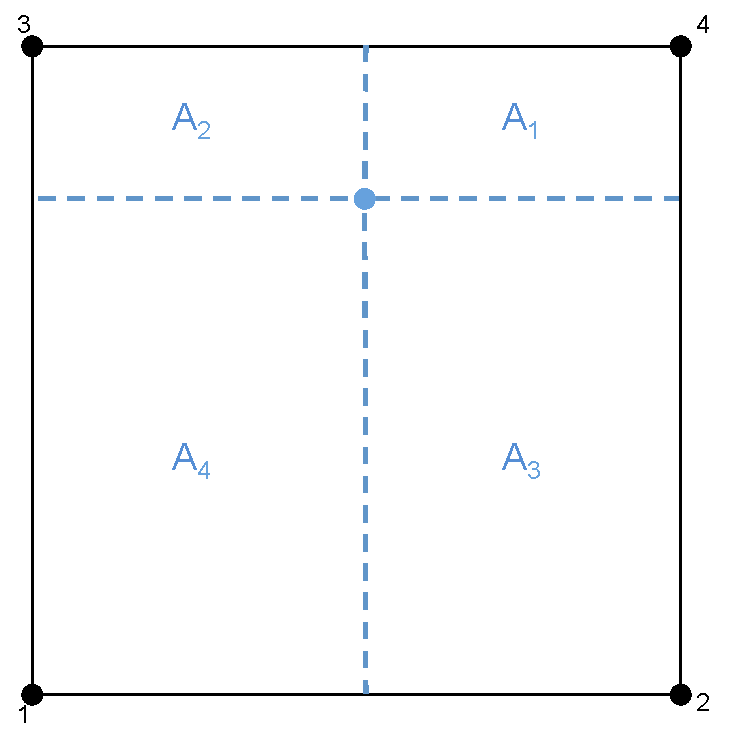
\includegraphics[height=2.5in]{./Multiscale/dRdxRVE.pdf}
\end{array}$
\end{center}
\caption{Two-dimensional schematic of $A_i/A$. Blue dot represents fiber node that lies on RVE face. Black dots represent the 4 nodes on an RVE face. The total area of the RVE face is $A=A_1+A_2+A_3+A_4$. }
\label{fig:dRdxRVE}
\end{figure}
%
\subsubsection{Derivative of $V$ with respect to RVE corner coordinates}

The volume can be calculated in the parent domain by
%
\begin{equation}
V = \int_{-1}^{1} \int_{-1}^1 \int_{-1}^1 \text{det}\pmb{J}^e d\xi_1 d\xi_2 d\xi_3  = \int_{-1}^{1} \left(\int_{-1}^1 \left(\int_{-1}^1 \text{det}\pmb{J}^e d\xi_1 \right)d\xi_2\right) d\xi_3 ,
\label{eq:volume}
\end{equation}
%
which has been written in terms of three consecutive integrals. In the biotissue code, the integrals are evaluated using the Gauss integration formula where Eq.\ \eqref{eq:volume} becomes 
%
\begin{equation}
V = \sum_{i=1}^{N_{gp}} \sum_{j=1}^{N_{gp}} \sum_{k=1}^{N_{gp}} W_i W_j W_k \text{det}\pmb{J}^e(\xi_1^{(i)},\xi_2^{(j)},\xi_3^{(k)})
\label{eq:gauss_integration}
\end{equation}
%
where $N_{gp}$ is the number of Gauss integration points, $W_i$ is the weight of the $i^{th}$ integration point, $\pmb{J}^e$ is the Jacobian matrix, and $\xi_i^{(j)}$ is the $i^{th}$ component of the $j^{th}$ integration point. Note that $V$ is the volume for a hexahedron where $N_{gp}=2$, $W_i=1$, and $\xi_i^{(j)}=\pm 1/\sqrt{3}$. 

The derivative of the Volume with respect to the RVE corner coordinates can be written in index notation as
%
\begin{eqnarray}
\frac{\partial V}{\partial x_l^{RVE}} &=& \int_{-1}^1 \int_{-1}^1 \int_{-1}^1 \frac{\partial}{\partial x_l^{RVE}} \left(\text{det}\pmb{J}^e\right) d\xi_1 d\xi_2 d\xi_3 \nonumber\\
%
&=& \sum_{i=1}^{N_{gp}} \sum_{j=1}^{N_{gp}} \sum_{k=1}^{N_{gp}} W_i W_j W_k \frac{\partial}{\partial x_l^{RVE}} \left(\text{det}\pmb{J}^e(\xi_1^{(i)},\xi_2^{(j)},\xi_3^{(k)})\right),
\label{eq:dVdvl}
\end{eqnarray}
%
where we have applied the Gauss integration formula (c.f., Eq.\ \eqref{eq:gauss_integration}). The derivative of det$\pmb{J}^e(\xi_1^{(i)},\xi_2^{(j)},\xi_3^{(k)})$ is 
%
\begin{eqnarray}
&&\frac{\partial}{\partial x_l^{RVE}}\left(\text{det}\pmb{J}^e(\xi_1^{(i)},\xi_2^{(j)},\xi_3^{(k)})\right) \nonumber\\
%
&&= \frac{\partial}{\partial x_l^{RVE}}\bigg[x_{,\xi_1}\left(y_{,\xi_2}z_{,\xi_3} - z_{,\xi_2}y_{,\xi_3} \right) - y_{,\xi_1}\left(x_{,\xi_2}z_{,\xi_3}-z_{,\xi_2}x_{,\xi_3} \right) + z_{,\xi_1}\left(x_{,\xi_2}y_{,\xi_3}-y_{,\xi_2}x_{,\xi_3} \right)\bigg] \bigg |_{\xi_1 = \xi_1^{(i)}, \xi_2 = \xi_2^{(j)}, \xi_3 = \xi_3^{(k)}}.  \nonumber\\
\end{eqnarray}
%
To illustrate, the $x, y, z$ components of the derivative for the ``first" node of the hexahedron $(x_1^{RVE},x_2^{RVE}, x_3^{RVE})$ are explicitly written out:
%
\begin{eqnarray}
\frac{\partial \text{det}\pmb{J}^e}{\partial x_1^{RVE}} &=& \frac{\partial x_{,\xi_1}}{\partial x_1^{RVE}}\left(y_{,\xi_2}z_{,\xi_3} - z_{,\xi_2}y_{,\xi_3} \right) - y_{,\xi_1}\left(\frac{\partial x_{,\xi_2}}{\partial x_1^{RVE}}z_{,\xi_3}-z_{,\xi_2}\frac{\partial x_{,\xi_3}}{\partial x_1^{RVE}} \right) + z_{,\xi_1}\left(x_{,\xi_2}y_{,\xi_3}-y_{,\xi_2}x_{,\xi_3} \right) \nonumber\\
%
&=& \text{det} \begin{bmatrix}
\frac{\partial x_{,\xi_1}}{\partial x_1^{RVE}} & y_{,\xi_1} & z_{,\xi_1} \\
\frac{\partial x_{,\xi_2}}{\partial x_1^{RVE}} & y_{,\xi_2} & z_{,\xi_2} \\
\frac{\partial x_{,\xi_3}}{\partial x_1^{RVE}} & y_{,\xi_3} & z_{,\xi_3}
\end{bmatrix} 
%
= \text{det} \begin{bmatrix}
\frac{\partial N_1^{6\text{hex}}}{\partial \xi_1} & y_{,\xi_1} & z_{,\xi_1} \\
\frac{\partial N_1^{6\text{hex}}}{\partial \xi_2} & y_{,\xi_2} & z_{,\xi_2} \\
\frac{\partial N_1^{6\text{hex}}}{\partial \xi_3} & y_{,\xi_3} & z_{,\xi_3}
\end{bmatrix} \nonumber\\
%%
\frac{\partial \text{det}\pmb{J}^e}{\partial x_2^{RVE}} &=& x_{,\xi_1}\left(\frac{\partial y_{,\xi_2}}{\partial x_2^{RVE}}z_{,\xi_3} - z_{,\xi_2}\frac{\partial y_{,\xi_3}}{\partial x_2^{RVE}} \right) - \frac{\partial y_{,\xi_1}}{\partial x_2^{RVE}}\left(x_{,\xi_2}z_{,\xi_3}-z_{,\xi_2}x_{,\xi_3} \right) + z_{,\xi_1}\left(x_{,\xi_2}\frac{\partial y_{,\xi_3}}{\partial x_2^{RVE}}-\frac{\partial y_{,\xi_2}}{\partial x_2^{RVE}}x_{,\xi_3} \right) \nonumber\\
%
&=& \text{det} \begin{bmatrix}
x_{,\xi_1} & \frac{\partial y_{,\xi_1}}{\partial x_2^{RVE}} & z_{,\xi_1} \\
x_{,\xi_2} & \frac{\partial y_{,\xi_2}}{\partial x_2^{RVE}} & z_{,\xi_2} \\
x_{,\xi_3} & \frac{\partial y_{,\xi_3}}{\partial x_2^{RVE}} & z_{,\xi_3}
\end{bmatrix} 
%
= \text{det} \begin{bmatrix}
x_{,\xi_1} & \frac{\partial N_2^{6\text{hex}}}{\partial \xi_1} & z_{,\xi_1} \\
x_{,\xi_2} & \frac{\partial N_2^{6\text{hex}}}{\partial \xi_2} & z_{,\xi_2} \\
x_{,\xi_3} & \frac{\partial N_2^{6\text{hex}}}{\partial \xi_3} &  z_{,\xi_3}
\end{bmatrix} \nonumber\\
%%
\frac{\partial \text{det}\pmb{J}^e}{\partial x_3^{RVE}} &=& x_{,\xi_1}\left(y_{,\xi_2} \frac{\partial z_{,\xi_3}}{\partial x_3^{RVE}} - \frac{\partial z_{,\xi_2}}{\partial x_3^{RVE}} y_{,\xi_3} \right) - y_{,\xi_1}\left(x_{,\xi_2}\frac{\partial z_{,\xi_3}}{\partial x_3^{RVE}} - \frac{\partial z_{,\xi_2}}{\partial x_3^{RVE}} x_{,\xi_3} \right) + \frac{\partial z_{,\xi_1}}{\partial x_3^{RVE}}\left(x_{,\xi_2}y_{,\xi_3}-y_{,\xi_2}x_{,\xi_3} \right) \nonumber\\
%
&=& \text{det} \begin{bmatrix}
x_{,\xi_1} & y_{,\xi_1} & \frac{\partial z_{,\xi_1}}{\partial x_2^{RVE}}  \\
x_{,\xi_2} & y_{,\xi_2} & \frac{\partial z_{,\xi_2}}{\partial x_2^{RVE}}  \\
x_{,\xi_3} & y_{,\xi_3} & \frac{\partial z_{,\xi_3}}{\partial x_2^{RVE}} 
\end{bmatrix} 
%
= \text{det} \begin{bmatrix}
x_{,\xi_1} & z_{,\xi_1} & \frac{\partial N_3^{6\text{hex}}}{\partial \xi_1}  \\
x_{,\xi_2} & z_{,\xi_2} & \frac{\partial N_3^{6\text{hex}}}{\partial \xi_2}  \\
x_{,\xi_3} & z_{,\xi_3}& \frac{\partial N_3^{6\text{hex}}}{\partial \xi_3} 
\end{bmatrix} .
\label{eq:ddetJdvl}
\end{eqnarray}
%
Note that the formula for the derivatives for each component of the ``second" to ``eighth" nodes of the hexahedron are essentially the same, with the only difference being the shape function: $N_{l}^{6\text{hex}}$ with $l=4$ to $24$ for components corresponding to the second to eighth nodes. The relationship $\partial x_{,\xi_i}/\partial x_j^{RVE} = \partial N_j^{6\text{hex}}/\partial \xi_i$ was used in Eq.\ \eqref{eq:ddetJdvl}.

\subsubsection{Derivative of RVE corner coordinates with respect to finite-element displacements}

The matrix $[\partial \pmb{x}^{RVE}/\partial \pmb{u}^k]$ has dimensions of 24 (8 RVE corner nodes $\times$ 3 dofs per node) $\times$ 12 (4 FE tetrahedron nodes $\times$ 3 dofs per node) for each element: 
%
\setcounter{MaxMatrixCols}{12}
\begin{eqnarray}
\bigg[ \frac{\partial \pmb{x}^{RVE}}{\partial \pmb{u}^k} \bigg] &=& 
\begin{bmatrix}
\frac{\partial x_1^{RVE}}{\partial u_1^k} & \frac{\partial x_1^{RVE}}{\partial u_2^k} & \frac{\partial x_1^{RVE}}{\partial u_3^k} & &
%
 \frac{\partial x_1^{RVE}}{\partial u_{10}^k} & \frac{\partial x_1^{RVE}}{\partial u_{11}^k} & \frac{\partial x_1^{RVE}}{\partial u_{12}^k} \\
%%%
\frac{\partial x_2^{RVE}}{\partial u_1^k} & \frac{\partial x_2^{RVE}}{\partial u_2^k} & \frac{\partial x_2^{RVE}}{\partial u_3^k} & \cdots &
%
\frac{\partial x_2^{RVE}}{\partial u_{10}^k} & \frac{\partial x_2^{RVE}}{\partial u_{11}^k} & \frac{\partial x_2^{RVE}}{\partial u_{12}^k} \\
%%%
\frac{\partial x_3^{RVE}}{\partial u_1^k} & \frac{\partial x_3^{RVE}}{\partial u_2^k} & \frac{\partial x_3^{RVE}}{\partial u_3^k} &  &
%
\frac{\partial x_3^{RVE}}{\partial u_{10}^k} & \frac{\partial x_3^{RVE}}{\partial u_{11}^k} & \frac{\partial x_3^{RVE}}{\partial u_{12}^k} \\
%%%
 & \vdots & & & & \vdots & \\
 %%%
\frac{\partial x_{22}^{RVE}}{\partial u_1^k} & \frac{\partial x_{22}^{RVE}}{\partial u_2^k} & \frac{\partial x_{22}^{RVE}}{\partial u_3^k} & &
%
 \frac{\partial x_{22}^{RVE}}{\partial u_{10}^k} & \frac{\partial x_{22}^{RVE}}{\partial u_{11}^k} & \frac{\partial x_{22}^{RVE}}{\partial u_{12}^k} \\
%%%
\frac{\partial x_{23}^{RVE}}{\partial u_1^k} & \frac{\partial x_{23}^{RVE}}{\partial u_2^k} & \frac{\partial x_{23}^{RVE}}{\partial u_3^k} & \cdots &
%
\frac{\partial x_{23}^{RVE}}{\partial u_{10}^k} & \frac{\partial x_{23}^{RVE}}{\partial u_{11}^k} & \frac{\partial x_{23}^{RVE}}{\partial u_{12}^k} \\
%%%
\frac{\partial x_{24}^{RVE}}{\partial u_1^k} & \frac{\partial x_{24}^{RVE}}{\partial u_2^k} & \frac{\partial x_{24}^{RVE}}{\partial u_3^k} &  &
%
\frac{\partial x_{24}^{RVE}}{\partial u_{10}^k} & \frac{\partial x_{24}^{RVE}}{\partial u_{11}^k} & \frac{\partial x_{24}^{RVE}}{\partial u_{12}^k} \\
\end{bmatrix} \nonumber\\
%
&=&\begin{bmatrix}
\Delta N_1^{(1)} \pmb{I}_{3\times3} & \Delta N_2^{(1)}\pmb{I}_{3\times3} & \Delta N_3^{(1)} \pmb{I}_{3\times3} & \Delta N_4^{(1)}\pmb{I}_{3\times3} \\
%
\Delta N_1^{(2)} \pmb{I}_{3\times3} & \Delta N_2^{(2)}\pmb{I}_{3\times3} & \Delta N_3^{(2)} \pmb{I}_{3\times3} & \Delta N_4^{(2)}\pmb{I}_{3\times3} \\
%
\Delta N_1^{(3)} \pmb{I}_{3\times3} & \Delta N_2^{(3)}\pmb{I}_{3\times3} & \Delta N_3^{(3)} \pmb{I}_{3\times3} & \Delta N_4^{(3)}\pmb{I}_{3\times3} \\
%
\Delta N_1^{(4)} \pmb{I}_{3\times3} & \Delta N_2^{(4)}\pmb{I}_{3\times3} & \Delta N_3^{(4)} \pmb{I}_{3\times3} & \Delta N_4^{(4)}\pmb{I}_{3\times3} \\
%
\Delta N_1^{(5)} \pmb{I}_{3\times3} & \Delta N_2^{(5)}\pmb{I}_{3\times3} & \Delta N_3^{(5)} \pmb{I}_{3\times3} & \Delta N_4^{(5)}\pmb{I}_{3\times3} \\
%
\Delta N_1^{(6)} \pmb{I}_{3\times3} & \Delta N_2^{(6)}\pmb{I}_{3\times3} & \Delta N_3^{(6)} \pmb{I}_{3\times3} & \Delta N_4^{(6)}\pmb{I}_{3\times3} \\
%
\Delta N_1^{(7)} \pmb{I}_{3\times3} & \Delta N_2^{(7)}\pmb{I}_{3\times3} & \Delta N_3^{(7)} \pmb{I}_{3\times3} & \Delta N_4^{(7)}\pmb{I}_{3\times3} \\
%
\Delta N_1^{(8)} \pmb{I}_{3\times3} & \Delta N_2^{(8)}\pmb{I}_{3\times3} & \Delta N_3^{(8)} \pmb{I}_{3\times3} & \Delta N_4^{(8)}\pmb{I}_{3\times3} 
\end{bmatrix},
\label{eq:dRVEdFE_matrix}
\end{eqnarray}
%
where
%
\begin{eqnarray}
\Delta N_j^{(k)} \pmb{I}_{3\times3} &\equiv&
\begin{bmatrix}
\Delta N_j^{(k)} & 0 & 0 \\
0 & \Delta N_j^{(k)} & 0 \\
0 & 0 & \Delta N_j^{(k)} 
\end{bmatrix} \nonumber\\
%
\Delta N_j^{(k)} &\equiv& N_j^{4\text{tet}}(\xi_1^k,\xi_2^k,\xi_3^k) - N_j^{4\text{tet}}(\xi_1^{gp},\xi_2^{gp},\xi_3^{gp}) .
\label{eq:DeltaN_j^k}
\end{eqnarray}
%
In the matrix of Eq.\ \eqref{eq:dRVEdFE_matrix}, each 3 $\times$ 3 submatrix describes the relationship between the degrees of freedom of an RVE corner node and a FE tetrahedron node. These relationships are approximated as 3 $\times$ 3 diagonal matrices where the diagonal terms are calculated as the difference between the $j^{th}$ ($j$ ranges from 1 to 4 for tetrahedron) shape function at the barycentric coordinate of the $k^{th}$ RVE corner-node and that at the barycentric coordinate of the Gauss integration point (c.f., Eq.\ \eqref{eq:DeltaN_j^k}). 

\part{Constitutive Relationships}
\chapter{Compressible Hyperelastic Constitutive Relation}
\chapterauthor{V. W. L. Chan}

\section{Strain Tensors}

The relationship between an elemental vector in the material configuration, $d\pmb{X}$, and the spatial configuration, $d\pmb{x}$ is given by the deformation gradient tensor $\pmb{F}$
%
\begin{equation}
d\pmb{x} = \pmb{F}d\pmb{X},
\label{eq:dx=FdX}
\end{equation}
%
where $\pmb{F}$ is a two-tensor defined as
%
\begin{eqnarray}
\pmb{F} = \sum_{i,j=1}^3 \frac{\partial x_i}{\partial X_j} \vec{e}_i \otimes \vec{E}_j =
%
\begin{bmatrix}
\frac{\partial x_1}{\partial X_1} & \frac{\partial x_1}{\partial X_2} & \frac{\partial x_1}{\partial X_3} \\
\frac{\partial x_2}{\partial X_1} & \frac{\partial x_2}{\partial X_2} & \frac{\partial x_2}{\partial X_3} \\
\frac{\partial x_3}{\partial X_1} & \frac{\partial x_3}{\partial X_2} & \frac{\partial x_3}{\partial X_3} 
\end{bmatrix}.
\label{eq:deformation-gradient}
\end{eqnarray}
%

To measure general deformation, consider two elemental vectors $d\pmb{X}_1$ and $d\pmb{X}_2$ as they deform to $d\pmb{x}_1$ and $d\pmb{x}_2$. Such a deformation will involve stretching and changes in angle between the two elemental vectors. To find strain, which involves only the stretch of the vectors, consider the dot products of elemental vectors
%
\begin{eqnarray}
d\pmb{x}_1 \cdot d\pmb{x}_2 &=& (\pmb{F} d\pmb{X}_1) \cdot (\pmb{F}d\pmb{X}_2) \nonumber\\
%
&=& d\pmb{X}_1 \cdot \pmb{F}^T\pmb{F} d\pmb{X}_2 \nonumber\\
&=& d\pmb{X}_1 \cdot \pmb{C} d\pmb{X}_2,
\end{eqnarray}
%
where Eq.\ \eqref{eq:dx=FdX} has been applied and $\pmb{C} \equiv \pmb{F}^T \pmb{F}$ is the right Cauchy-Green deformation tensor (note that $\pmb{F}$ is on right side). One can also express the inverse relationship
%
\begin{eqnarray}
d\pmb{X}_1 \cdot d\pmb{X}_2 &=& (\pmb{F}^{-1}d\pmb{x}_1) \cdot (\pmb{F}^{-1} d\pmb{x}_2) \nonumber\\
&=& d\pmb{x}_1 \cdot (\pmb{F}^{-1})^T\pmb{F}^{-1} d\pmb{x}_2 \nonumber\\
&=& d\pmb{x}_1 \cdot \pmb{b}^{-1} d\pmb{x}_2,
\end{eqnarray}
%
where $\pmb{b} \equiv \pmb{F}\pmb{F}^T = (\pmb{b}^{-1})^{-1} = ((\pmb{F}^T)^{-1} \pmb{F}^{-1})^{-1}$ is the left Cauchy-Green deformation tensor (note that $\pmb{F}$ is on left side).

The strain can be defined as the change of length from the material to spatial configuration
%
\begin{eqnarray}
\frac{1}{2}\left(d\pmb{x}_1 \cdot d\pmb{x}_2 - d\pmb{X}_1 \cdot d\pmb{X}_2 \right) &=& \frac{1}{2}\left(d\pmb{X}_1 \cdot \pmb{C} d\pmb{X}_2 - d\pmb{X}_1 \cdot d\pmb{X}_2 \right) = d\pmb{X}_1 \cdot \pmb{E} d\pmb{X}_2 \nonumber\\
%
&=& \frac{1}{2}\left(d\pmb{x}_1 \cdot d\pmb{x}_2 - d\pmb{x}_1 \cdot \pmb{b}^{-1} d\pmb{x}_2\right) = d\pmb{x}_1 \cdot \pmb{e} d\pmb{x}_2, \nonumber\\
%
\text{where}&&\nonumber\\
%
\pmb{E} &\equiv& \frac{1}{2} \left(\pmb{C} - \pmb{I} \right) \ \ \text{and} \ \ \pmb{e} \equiv \frac{1}{2}\left(\pmb{I} - \pmb{b}^{-1}\right)
\end{eqnarray}
%
are Lagrangian (or Green) and Eulerian (or Almansi) strain tensors, respectively.

\section{Elasticity Tensors}

In the case when work done by the stresses during deformation only depend on the initial and final configurations, the behavior of the material is called path-independent. Elastic materials that are path-independent are termed hyperelastic. As a consequence of the path-independent behavior, an elastic potential $\Psi$ per unit undeformed volume can be defined as
%
\begin{equation}
\Psi(\pmb{F}(\pmb{X}),\pmb{X}) = \int_{t_0}^t \pmb{P}(\pmb{F}(\pmb{X}),\pmb{X}):\dot{\pmb{F}}dt \ \text{ and } \ \dot{\Psi} = \pmb{P} : \dot{\pmb{F}} = \sum_{i,j=1}^3\frac{\partial \Psi}{\partial F_{ij}}\dot{F}_{ij},
\label{eq:hyperelastic}
\end{equation}
%  
where $\pmb{P}$ is the first Piola-Kirchhoff stress tensor (work conjugate to the rate of deformation gradient $\dot{\pmb{F}}$). Equation \eqref{eq:hyperelastic} is often used as a definition for hyperelastic materials \cite{JavierBonet:2008uxa}. Considering the restrictions imposed by objectivity, $\Psi$ can be expressed in terms of the right Cauchy-Green deformation tensor \pmb{C}
%
\begin{eqnarray}
\Psi(\pmb{C}(\pmb{X}),\pmb{X}) = \int_{t_0}^t \pmb{S}(\pmb{C}(\pmb{X}),\pmb{X}) : \dot{\pmb{C}} dt \ \text{ and } \ \dot{\Psi} =  \frac{1}{2}\pmb{S}:\dot{\pmb{F}} = \sum_{i,j=1}^3\frac{\partial \Psi}{\partial C_{ij}}\dot{C}_{ij} = \frac{1}{2} \sum_{i,j=1}^3\frac{\partial \Psi}{\partial E_{ij}}\dot{C}_{ij}, 
\end{eqnarray}
%
where $\pmb{S}$ is the second Piola-Kirchhoff stress tensor (work conjugate to the rate of right Cauchy-Green deformation \pmb{C}) and $\pmb{E} = 1/2(\pmb{C}-\pmb{I})$ is the Lagrangian strain tensor.

The relationship between $\pmb{S}$ and $\pmb{C}$ or $\pmb{E}$ is nonlinear. A linear relationship can be obtained by taking the directional derivative of $\pmb{S}$
%
\begin{eqnarray}
DS_{IJ}[\pmb{u}] &=& \frac{d}{d\epsilon}\bigg|_{\epsilon=0}S_{IJ}(E_{KL}[\phi+\epsilon \pmb{u}]) \nonumber\\
%
&=& \sum_{K,L=1}^3 \frac{\partial S_{IJ}}{\partial E_{KL}}\frac{d}{d\epsilon}\bigg|_{\epsilon=0}E_{KL}[\phi+\epsilon \pmb{u}] \nonumber\\
%
&=&  \sum_{K,L=1}^3 \frac{\partial S_{IJ}}{\partial E_{KL}} DE_{KL}[\pmb{u}],
\label{eq:DS[u]}
\end{eqnarray}
%
where the chain rule has been applied in the second line and $DE_{K,L}[\pmb{u}]$ is the directional derivative of $E_{KL}$. More concisely, Eq.\ \eqref{eq:DS[u]} is
%
\begin{equation}
D\pmb{S}[\pmb{u}] = \pmb{\mathbb{C}}:D\pmb{E}[\pmb{u}],
\label{eq:DS[u]_compact}
\end{equation}
%
where $\pmb{\mathbb{C}}$ is the fourth-order Lagrangian (or material) elasticity tensor
%
\begin{equation}
\pmb{\mathbb{C}} \equiv \sum_{I,J,K,L=1}^3 \frac{\partial S_{IJ}}{\partial E_{KL}} \vec{E}_I \otimes \vec{E}_J \otimes \vec{E}_K \otimes \vec{E}_L = 2\frac{\partial \pmb{S}}{\partial \pmb{C}} = 4\frac{\partial^2 \Psi}{\partial \pmb{C} \partial \pmb{C}}.
\end{equation}
%
The spatial equivalent of $\pmb{\mathbb{C}}$ can be obtained by applying the push forward operation on the rate form of Eq.\ \eqref{eq:DS[u]_compact} to obtain \cite{JavierBonet:2008uxa}
%
\begin{equation}
\pmb{\sigma}^o = \pmb{c}:\pmb{d},
\end{equation}
%
where $\pmb{\sigma}^o$ is the Truesdell stress rate, $\pmb{d}$ is the rate of deformation tensor, $\pmb{c}$ is the Eulerian (or spatial) elasticity tensor
%
\begin{equation}
\pmb{c} \equiv \sum_{i,j,k,l,I,J,K,L=1}^3 J^{-1} F_{iI} F_{jJ} F_{kK} F_{lL} C_{IJKL} \vec{e}_i \otimes \vec{e}_j \otimes \vec{e}_k \otimes \vec{e}_l.
\end{equation}
%
\section{Isotropic Hyperelasticity}

The hyperelastic constitutive equations discussed in the previous section are unrestricted. Here, the constitutive equations are restricted to be isotropic, i.e., the constitutive behavior to be identical in any material direction. Consequently, the elastic potential must be a function of only invariants of $\pmb{C}: \Psi(I_C,II_C,III_C,\pmb{X})$. The invariant of $\pmb{C}$ are
%
\begin{eqnarray}
I_C &=& \text{tr}\pmb{C} = \pmb{C}:\pmb{I} \nonumber\\
II_C &=& \text{tr}\pmb{C}\pmb{C} = \pmb{C}:\pmb{C} \nonumber\\
III_C &=& \text{det}\pmb{C} = J^2 .
\label{eq:invariants}
\end{eqnarray}
%
As a result of the isotropic restriction, the second Piola-Kirchhoff stress tensor becomes
%
\begin{eqnarray}
\pmb{S} = 2\frac{\partial \Psi}{\partial \pmb{C}} &=& 2 \frac{\partial \Psi}{\partial I_C}\frac{\partial I_C}{\partial \pmb{C}} + 2\frac{\partial \Psi}{\partial II_C}\frac{\partial II_C}{\partial \pmb{C}} + 2\frac{\partial \Psi}{\partial III_C}\frac{\partial III_C}{\partial \pmb{C}} \nonumber\\
%%
&=&2\Psi_I \pmb{I} + 4\Psi_{II} \pmb{C} + 2J^2\Psi_{III}\pmb{C}^{-1},
\end{eqnarray}
%
where $\Psi_I = \partial \Psi/\partial I_C, \Psi_{II} = \partial \Psi/\partial II_C$, and $\Psi_{III} = \partial \Psi/\partial III_C$. Applying the relationship $\pmb{\sigma} = J^{-1}\pmb{F}\pmb{S}\pmb{F}^T$, the Cauchy stress can be expressed as
%
\begin{equation}
\pmb{\sigma} = 2J^{-1}\Psi_I \pmb{b} + 4J^{-1}\Psi_{II} \pmb{b}^2 + 2J\Psi_{III} \pmb{I}.
\label{eq:sigma_isotropic}
\end{equation}


\section{Compressible Neo-Hookean}

A compressible Neo-Hookean material is a simple case of an isotropic hyperelastic material. The elastic potential of a compressible Neo-Hookean material is
%
\begin{equation}
\Psi = \frac{\mu}{2} (I_C-3) - \mu \ln J + \frac{\lambda}{2}(\ln J)^2,
\label{eq:potential_neohookean}
\end{equation}
%
where $J^2 = III_C$ and the constants $\lambda$ and $\mu$ are the Lam\'e parameters:
%
\begin{align}
&\mu = \text{Shear Modulus} \nonumber\\
&\lambda = \frac{2 \mu \nu}{1- 2 \nu} \nonumber\\
&\nu = \text{Poisson Ratio}.
\label{eq:lame_parameters}
\end{align}
%
Note that in the absence of deformation (i.e., \pmb{C}=\pmb{I}), $\Psi=0$. Applying Eq.\ \eqref{eq:sigma_isotropic} to Eq.\ \eqref{eq:potential_neohookean}, the Cauchy stress is
%
\begin{eqnarray}
\pmb{\sigma} &=&  2J^{-1}\frac{\partial \Psi}{\partial I_C} \pmb{b} + 4J^{-1} \frac{\partial \Psi}{\partial II_C} \pmb{b}^2 + 2J\frac{\partial \Psi}{\partial III_C} \pmb{I} \nonumber\\
%
&=& 2J^{-1} \left(\frac{\mu}{2}\right)\pmb{b} + 4J^{-1} (0) \pmb{b}^2 + 2J\left(-\frac{\mu}{2}J^{-2}+\frac{\lambda}{2} J^{-2} \ln J \right)\pmb{I}  \nonumber\\
%
&=& \frac{\mu}{J}(\pmb{b} - \pmb{I}) + \frac{\lambda}{J}(\ln J) \pmb{I}.
\label{eq:NeoHookean_stress}
\end{eqnarray}
%
Comparing to the Neo-Hookean constitutive equation used in Lai et al.\ \cite{Lai:2013fp}, $\mu$ is the shear modulus and $\lambda \equiv (2\mu \nu)/(1-2\nu)$ where $\nu$ is Poisson's ratio.

The corresponding Eulerian elasticity tensor for the Neo-Hookean material can obtained by a push forward operation of the Lagrangian elasticity tensor to obtain \cite{JavierBonet:2008uxa}
%
\begin{equation}
\pmb{c}_{ijkl} = \lambda'\delta_{ij}\delta_{kl} + \mu' (\delta_{ik}\delta_{jl} + \delta_{il}\delta_{jk}),
\end{equation}
%
where $\lambda'$ and $\mu'$ are effective Lame moduli
%
\begin{equation}
\lambda' \equiv \frac{\mu}{J} \ \text{ and } \ \mu' \equiv \frac{\mu-\lambda \ln J}{J}.
\end{equation}
%

\section{Transversely Isotropic Neo-Hookean Material}

The elastic potential for a transversely isotropic Neo-Hookean material is \cite{Bonet:1998vc}
%
\begin{align}
&\Psi = \Psi_{\text{nh}} + \Psi_{\text{trns}} \nonumber\\ \ \
&\Psi_{\text{nh}} = \frac{\mu}{2}\left(I_C - 3\right) - \mu \ln(J) + \frac{\lambda}{2}\left(J - 1\right)^2 \nonumber\\ \ \
&\Psi_{\text{trns}} = \left[ \alpha + \beta \ln(J) + \gamma (IV_C - 1)\right] (IV_C - 1) - \frac{\alpha}{2}\left(V_C - 1\right), 
\label{eq:psi_trns_iso}
\end{align}
%
where $IV_C$ and $V_C$ are two new scalars defined in terms of the right Cauchy-Green deformation tensor $\pmb{C}$ and the axial direction vector $\pmb{A}$ as
%
\begin{align}
&IV_C \equiv \pmb{A} \cdot \pmb{C} \pmb{A} = \pmb{A}\cdot(\pmb{F}^T\pmb{F})\pmb{A} = (\pmb{F}\pmb{A})\cdot(\pmb{F}\pmb{A}) = \pmb{a} \cdot \pmb{a} \nonumber\\
&V_C \equiv \pmb{A} \cdot \pmb{C}^2 \pmb{A} .
\label{eq:invariants_trns_iso}
\end{align}
%

The Cauchy-stress tensor $\pmb{\sigma}$ can be derived from the elastic potential as
%
\begin{align}
&J\pmb{\sigma} = \pmb{F} \left(\pmb{S}_{\text{nh}} + \pmb{S}_{\text{trns}}\right)\pmb{F}^T = J\pmb{\sigma}_{\text{nh}} +J\pmb{\sigma}_{\text{trns}} \nonumber\\ \ \
%
&\pmb{\sigma}_{\text{nh}} = \frac{\mu}{J}\left(\pmb{b} - \pmb{I}\right) + \lambda \left(J - 1\right) \pmb{I} \nonumber\\ \ \
%
&\pmb{\sigma}_{\text{trns}} = \frac{2\beta}{J}\left(\pmb{a}\cdot\pmb{a} -1\right)\pmb{I} + \frac{2}{J}\left[\alpha + 2\beta \ln J + 2\gamma(\pmb{a}\cdot\pmb{a}-1) \right] \pmb{a} \otimes \pmb{a} - \frac{\alpha}{J}(\pmb{b}\pmb{a}\otimes\pmb{a} + \pmb{a} \otimes \pmb{b} \pmb{a}),
\label{eq:cauchy_stress_trns_iso}
\end{align}
%
where the definitions for $I_C=\pmb{C}:\pmb{I}$ in Eq.\ \eqref{eq:invariants} and $IV_C=\pmb{a}\cdot\pmb{a}$ in Eq.\ \eqref{eq:invariants_trns_iso} have been used. The corresponding spatial elasticity tensor is
\begin{align}
&\pmb{c} = \pmb{c}_{\text{nh}} + \pmb{c}_{\text{trns}} \nonumber\\
%
&\pmb{c}_{\text{nh}} = \lambda(2J-1)\pmb{I} \otimes \pmb{I}+\frac{2}{J}\left[\mu - \lambda J(2J-1)\right]\pmb{i} \nonumber\\ \ \
%
&\pmb{c}_{\text{trns}} = \frac{8\gamma}{J}\pmb{a} \otimes \pmb{a} \otimes \pmb{a} \otimes \pmb{a} + \frac{4\beta}{J}\left(\pmb{a}\otimes\pmb{a}\otimes\pmb{I}+\pmb{I}\otimes\pmb{a}\otimes\pmb{a} \right) - \frac{\alpha}{J} \textbf{a} - \frac{4\beta}{J}(\pmb{a}\cdot\pmb{a}-1)\pmb{i} \nonumber\\ \ \
%
&\pmb{i} \equiv \delta_{ik}\delta_{jl} \nonumber\\
%
&\textbf{a} \equiv a_i a_l b_{jk} + b_{ik} a_j a_l,
\label{eq:c_trns_iso}
\end{align}
%
where the definition for $IV_C=\pmb{a}\cdot\pmb{a}$ in Eq.\ \eqref{eq:invariants_trns_iso} has been used. The constants of Eqs.\ \eqref{eq:cauchy_stress_trns_iso} and \eqref{eq:c_trns_iso} are \cite{Bonet:1998vc}
%
\begin{align}
&\lambda = \frac{2\mu (\nu+n\nu^2)}{m} \nonumber\\ 
%
&\mu = \text{Shear Modulus} \nonumber\\
%
&\alpha = \mu - G_A \nonumber\\
%
&\beta = \frac{\mu \nu^2(1-n)}{2m} \nonumber\\ 
%
&\gamma = \frac{E_A(1-\nu)}{8m} - \frac{\lambda+2\mu}{8} + \frac{\alpha}{2} - \beta \nonumber\\
%
&m = 1 - \nu - 2 n\nu^2 \nonumber\\
%
&n = \frac{E_A}{2\mu(1+\nu)},
\label{eq:trns_iso_constants}
\end{align}
%
where the input parameters to the integrator are shear modulus ($\mu$), axial shear modulus ($G_A$), the Poisson ratio ($\nu$), and the axial Young's modulus ($E_A$).  

The stress and elasticity tensors in Eqs.\ \eqref{eq:cauchy_stress_trns_iso} and \eqref{eq:c_trns_iso} can be rewritten in the more convenient indicial form
%
\begin{align}
&\sigma^{\text{nh}}_{ij} = \frac{\mu}{J}(b_{ij} - \delta_{ij}) + \lambda(J-1)\delta_{ij} \nonumber\\
%
&\sigma^{\text{trns}}_{ij} = \frac{2\beta}{J}(a_r a_r - 1)\delta_{ij} + \frac{2}{J}[\alpha+2\beta\ln J+2\gamma(a_r a_r -1)]a_i a_j - \frac{\alpha}{J}(b_{is}a_s a_j+a_i b_{jr}a_r) \nonumber\\
%
&c^{\text{nh}}_{ijkl} = \lambda(2J-1)\delta_{ij}\delta_{kl} + \frac{2}{J}[\mu - \lambda J(2J-1)]\delta_{ik}\delta_{jl} \nonumber\\
%
&c^{\text{trns}}_{ijkl} = \frac{8\gamma}{J}a_i a_j a_k a_l + \frac{4\beta}{J}(a_i a_j \delta_{kl} + \delta_{ij}a_k a_l) - \frac{\alpha}{J}(a_i a_l b_{jk} + b_{ik}a_j a_l) - \frac{4\beta}{J}(a_r a_r - 1)\delta_{ik}\delta_{jl}.
\label{eq:inidicial_form}
\end{align}
%
In the multiscale code, the stress tensor are written as a vector using Voigt format
%
\begin{equation}
\hat{\pmb{\sigma}} \equiv  [\sigma_{11}, \sigma_{22}, \sigma_{33}, \sigma_{12}, \sigma_{23}, \sigma_{13}]^T
\end{equation}
%
Therefore, the elasticity tensor is represented as a symmetric 6 $\times$ 6 matrix via Voigt format as
%
\begin{eqnarray}
\hat{\pmb{c}} \equiv 
\begin{bmatrix}
c_{1111} & c_{1122} & c_{1133} & c_{1112} & c_{1123} & c_{1113} \\
              & c_{2222} & c_{2233} & c_{2212} & c_{2223} & c_{2213} \\
              &                & c_{3333} & c_{3312} & c_{3323} & c_{3313} \\
              &                &                & c_{1212} & c_{1223} & c_{1213} \\
              &                &                &                & c_{2323} & c_{2313} \\
              &                &                &                &                & c_{1313}       
\end{bmatrix}
\end{eqnarray}
% 
%%%%%%%
\section{Linearized Equilibrium Equations}

The internal virtual work can be expressed in a Lagrangian form via
%
\begin{equation}
\delta W_{int}(\phi,\delta \pmb{v}) = \int_V \pmb{S} : \delta \dot{\pmb{E}}dV,
\end{equation}
%
demonstrating that the \textit{second Piola-Kirchhoff stress tensor} $\pmb{S}$ is the work conjugate to the \textit{material strain rate tensor} $\dot{\pmb{E}}$. The corresponding directional derivative is
%
\begin{eqnarray}
D\delta W_{int}(\phi,\delta \pmb{v})[\pmb{u}] &=& \int_V D(\pmb{S}:\delta \dot{\pmb{E}})[\pmb{u}]dV \nonumber\\
%
&=& \int_V D\pmb{S}[\pmb{u}]:\delta \dot{\pmb{E}}dV +  \int_V \pmb{S}: D\delta \dot{\pmb{E}}[\pmb{u}]dV \nonumber\\
%
&=& \int_V \delta \dot{\pmb{E}}:\pmb{\mathbb{C}}:D\pmb{E}[\pmb{u}] +  \int_V \pmb{S}: D\delta \dot{\pmb{E}}[\pmb{u}]dV \nonumber\\
%
&=& \int_V \delta \dot{\pmb{E}}:\pmb{\mathbb{C}}:D\pmb{E}[\pmb{u}] +  \int_V \pmb{S}: [(\nabla_0 \pmb{u})^T \nabla_0\delta \pmb{v}]dV,
\label{eq:DW[u]_Lagrangian1}
\end{eqnarray}
%
where the product rule has been used in the second line, the relationship for $D\pmb{S}[\pmb{u}]$ in Eq.\ \eqref{eq:DS[u]_compact} for the third line, and the relationship
%
\begin{equation}
D\delta \dot{\pmb{E}}[\pmb{u}] = \frac{1}{2}[(\nabla_0 \delta \pmb{v})^T\nabla_0 \pmb{u} + (\nabla_0 \pmb{u})^T\nabla_0\delta \pmb{v}]
%
= (\nabla_0 \pmb{u})^T \nabla_0\delta \pmb{v}
\end{equation}
%
is used in the last line. Furthermore, noting that $D\pmb{E}[\delta \pmb{v}] = \delta \dot{\pmb{E}}$, Eq.\ \eqref{eq:DW[u]_Lagrangian1} can be rewritten as
%
\begin{equation}
D\delta W_{int}(\phi,\delta \pmb{v})[\pmb{u}] = \int_V D\pmb{E}[\delta\pmb{v}] :\pmb{\mathbb{C}}:D\pmb{E}[\pmb{u}] +  \int_V \pmb{S}: [(\nabla_0 \pmb{u})^T \nabla_0\delta \pmb{v}]dV.
\label{eq:DW[u]_Lagrangian}
\end{equation}
%

The linearized equilibrium equation of Eq.\ \eqref{eq:DW[u]_Lagrangian} can be simplified to expressing in the Eulerian (or spatial) form. This is achieved by push-forward and pull-back operations on the individual terms to obtain (see Section 8.4 of Ref.\ \cite{JavierBonet:2008uxa})
%
\begin{eqnarray}
D\pmb{E}[\delta\pmb{v}] :\pmb{\mathbb{C}}:D\pmb{E}[\pmb{u}]dV &=& \delta \pmb{d}:\pmb{c}:\varepsilon dv \nonumber\\
%
\pmb{S}: [(\nabla_0 \pmb{u})^T \nabla_0\delta \pmb{v}]dV &=& \pmb{\sigma}:[(\nabla \pmb{u})^T\nabla \delta \pmb{v}],
\label{eq:pushback_pullforward_results}
\end{eqnarray}
%
where $\varepsilon = 1/2[\nabla \pmb{u} + (\nabla \pmb{u})^T]$ is the \textit{small-strain tensor}. Applying the relationships in Eq.\ \eqref{eq:pushback_pullforward_results}, the Eulerian form of the linearized equilibrium equation is
%
\begin{equation}
D\delta W_{int}(\phi,\delta \pmb{v})[\pmb{u}] = \int_v \delta \pmb{d}:\pmb{c}:\varepsilon dv + \int_v \pmb{\sigma}:[(\nabla \pmb{u})^T\nabla \delta \pmb{v}]dv.
\label{eq:DW[u]_Eulerian}
\end{equation}
%
Note that 
%
\begin{equation}
\delta \pmb{d} = \frac{1}{2}(\nabla \delta \pmb{v} + (\nabla \delta \pmb{v})^T),
\end{equation}
%
which is the same functional form between $\varepsilon$ and $\pmb{u}$. This together with the fact that $\pmb{c}$ and $\pmb{\sigma}$ are symmetric implies that $\pmb{u}$ and $\delta \pmb{v}$ can be interchanged without altering results (how can I show this??)
%
\begin{equation}
D\delta W_{int}(\phi,\delta \pmb{v})[\pmb{u}] = D\delta W_{int}(\phi,\pmb{u})[\delta \pmb{v}] .
\end{equation}
%
Such a symmetry gives rise to a symmetric tangent-stiffness matrix upon discretization.

\section{Discretization of Linearized Equilibrium Equations}

\subsection{Isoparametric Elements}

To discretize the linearized virtual work equation in Eq.\ \eqref{eq:DW[u]_Eulerian}, isoparametric elements are used to interpolate the current position in terms of current nodal position $\pmb{x}_a$
%
\begin{equation}
\pmb{x} = \sum_{a=1}^n N_a \pmb{x}_a(t),
\label{eq:interpolate_position}
\end{equation}
% 
where $N_a(\xi_1,\xi_2,\xi_3)$ are the shape functions and $n$ denotes the number of nodes per element. Differentiating Eq.\ \eqref{eq:interpolate_position} with respect to time gives real and virtual velocity interpolations
%
\begin{equation}
\pmb{v} = \sum_{a=1}^n N_a \pmb{v}_a \ \ \text{ and } \ \ \delta \pmb{v} = \sum_{a=1}^n N_a \delta \pmb{v}_a,
\label{eq:interpolate_velocity}
\end{equation}
%
respectively.  Similarly, restricting the motion brought about by an arbitrary increment $\pmb{u}$ according Eq.\ \eqref{eq:interpolate_position} implies that the displacement is interpolated as follows
%
\begin{equation}
\pmb{u} = \sum_{a=1}^n N_a \pmb{u}_a.
\label{eq:interpolate_displacement}
\end{equation}
%

Using Eq.\ \eqref{eq:interpolate_velocity} the real and virtual velocity gradient can also be written in terms of the shape functions as
%
\begin{eqnarray}
\pmb{l} = \nabla \pmb{v} &=& \sum_{i,j=1}^3 \frac{\partial v_i}{\partial x_j} \vec{e}_i \otimes \vec{e}_j = \begin{bmatrix}
\frac{\partial v_1}{\partial x_1} & \frac{\partial v_1}{\partial x_2} & \frac{\partial v_1}{\partial x_3} \\
\frac{\partial v_2}{\partial x_1} & \frac{\partial v_2}{\partial x_2} & \frac{\partial v_2}{\partial x_3} \\
\frac{\partial v_3}{\partial x_1} & \frac{\partial v_3}{\partial x_2} & \frac{\partial v_3}{\partial x_3} 
\end{bmatrix} \nonumber\\
%
&=&\sum_{a=1}^n \begin{bmatrix}
\frac{\partial N_a }{\partial x_1}v_{1a} & \frac{\partial N_a}{\partial x_2}v_{1a} & \frac{\partial N_a}{\partial x_3}v_{1a} \\
\frac{\partial N_a }{\partial x_1}v_{2a} & \frac{\partial N_a}{\partial x_2}v_{2a} & \frac{\partial N_a}{\partial x_3}v_{2a} \\
\frac{\partial N_a }{\partial x_1}v_{3a} & \frac{\partial N_a}{\partial x_2}v_{3a} & \frac{\partial N_a}{\partial x_3}v_{3a} 
\end{bmatrix} \nonumber\\
%
&=& \sum_{a=1}^n \pmb{v}_a \otimes \nabla N_a,
\label{eq:interpolate_velgrad}
\end{eqnarray}
%
similarly
%
\begin{equation}
\delta \pmb{l} = \sum_{a=1}^n \delta \pmb{v}_a \otimes N_a.
\label{eq:interpolate_virtual_velgrad}
\end{equation}
%
Furthermore, applying Eq.\ \eqref{eq:interpolate_virtual_velgrad} the virtual displacement rate tensor is
%
\begin{eqnarray}
\delta \pmb{d} = \frac{1}{2}\left(\delta \pmb{l} + \delta \pmb{l}^T\right) = \frac{1}{2}\sum_{a=1}^n \left(\delta \pmb{v}_a \otimes \nabla N_a + \nabla N_a \otimes \delta \pmb{v}_a\right).
\label{eq:interpolate_displacement_rate}
\end{eqnarray}
%
The deformation gradient tensor, which is used to calculate the Cauchy stress tensor in Eq.\ \eqref{eq:NeoHookean_stress}, can also be written in terms of the shape functions as
%
\begin{eqnarray}
\pmb{F} &=& \sum_{i,I=1}^3 F_{iI}\vec{e}_i \otimes \vec{E}_I =
%
\begin{bmatrix}
F_{11} & F_{12} & F_{13} \\
F_{21} & F_{22} & F_{23} \\
F_{31} & F_{32} & F_{33}
\end{bmatrix}, \ \text{ where } \ \nonumber\\
%
F_{iI} &=& \frac{\partial x_i}{\partial X_I} = \sum_{a=1}^nx_{a,i}\frac{\partial N_a }{\partial X_{a,I}}.
\end{eqnarray}
% 

Next consider the the linearized virtual work for element $(e)$ linking nodes $a$ and $b$. Specifically, the constitutive and initial stress components of Eq.\ \eqref{eq:DW[u]_Eulerian} are examined separately.

\subsection{Constitutive Component}

The first term on the right-hand-side of Eq.\ \eqref{eq:DW[u]_Eulerian} is the constitutive component. Its contribution for element $(e)$ linking nodes $a$ and $b$ is
%
\begin{equation}
D\delta W_c^{(e)}(\phi,N_a\delta \pmb{v}_a)[N_b\pmb{u}_b] = \int_{v^{(e)}} \frac{1}{2} \left(\delta \pmb{v}_a \otimes \nabla N_a + \nabla N_a \otimes \delta \pmb{v}_a\right):\pmb{c}:\frac{1}{2} \left(\delta \pmb{u}_b \otimes \nabla N_b + \nabla N_b \otimes \delta \pmb{v}_b\right)dv.
\label{eq:DW_c[u]_discretize}
\end{equation}
%
Equation \eqref{eq:DW_c[u]_discretize} can be written in matrix-vector (also known as Voigt) notation by reinterpreting small-strain tensor $\varepsilon$ as
%
\begin{equation}
\hat{\varepsilon} \equiv [\varepsilon_{11}, \varepsilon_{22}, \varepsilon_{33}, 2\varepsilon_{12}, 2\varepsilon_{23}, 2\varepsilon_{13}]^T = \sum_{a=1}^n \pmb{B}_a \pmb{u}_a
\label{eq:strain_Voigt}
\end{equation}
%
and the virtual displacement rate tensor as
%
\begin{equation}
\delta\hat{\pmb{d}} \equiv [\delta d_{11}, \delta d_{22}, \delta d_{33}, 2\delta d_{12}, 2\delta d_{23}, 2\delta d_{13}]^T = \sum_{a=1}^n \pmb{B}_a \delta \pmb{v}_a,
\label{eq:virtual_displacement_Voigt}
\end{equation}
%
where $\pmb{B}_a$ is defined in terms of derivatives of the shape functions as
%
\begin{equation}
\pmb{B}_a \equiv
\begin{bmatrix}
\frac{\partial N_a}{\partial x_1} & 0 & 0  \\
0 & \frac{\partial N_a}{\partial x_2} & 0 \\
0 & 0 & \frac{\partial N_a}{\partial x_3} \\
\frac{\partial N_a}{\partial x_2} & \frac{\partial N_a}{\partial x_1} & 0  \\ 
0 & \frac{\partial N_a}{\partial x_3} & \frac{\partial N_a}{\partial x_2}  \\
\frac{\partial N_a}{\partial x_3} & 0 & \frac{\partial N_a}{\partial x_1} 
\end{bmatrix}.
\end{equation}
%
Note that the definition of $\pmb{B}_a$ is different from Ref.\ \cite{JavierBonet:2008uxa} because the ordering of the small-strain and virtual displacement rate tensor components in Eqs.\ \eqref{eq:strain_Voigt} and \eqref{eq:virtual_displacement_Voigt} is different from what is presented in Ref.\ \cite{JavierBonet:2008uxa}. Applying Voigt notation, Eq.\ \eqref{eq:DW_c[u]_discretize} is simplified to
%
\begin{eqnarray}
D\delta W_c^{(e)}(\phi,N_a\delta \pmb{v}_a)[N_b\pmb{u}_b] &=& \int_{v^{(e)}}(\pmb{B}_a \delta \pmb{v}_a)^T \pmb{D} (\pmb{B}_b \pmb{u}_b) dv \nonumber\\
%
&=& \delta \pmb{v}_a \cdot \left(\int_{v^{(e)}} \pmb{B}_a^T \pmb{D} \pmb{B}_b  dv \right)\pmb{u}_b \nonumber\\
%
&=& \delta \pmb{v}_a \cdot \pmb{K}^{(e)}_{c,ab} \pmb{u}_a,
\end{eqnarray}
%
where
%
\begin{equation}
\pmb{D} = \begin{bmatrix}
\lambda' + 2\mu' & \lambda' & \lambda' & 0 & 0 & 0 \\
\lambda' & \lambda'+2\mu' & \lambda' & 0 & 0 & 0 \\
\lambda' & \lambda' & \lambda'+2\mu' & 0 & 0 & 0 \\
0 & 0 & 0 & \mu' & 0 & 0  \\
0 & 0 & 0 & 0 & \mu' & 0 \\
0 & 0 & 0 & 0 & 0 & \mu'  
\end{bmatrix}, \ \text{ where } \ \lambda' = \frac{\lambda}{\text{det}\pmb{J}} \ \text{ and } \ \mu' = \frac{\mu - \lambda \ln(\text{det}\pmb{J})}{\text{det}\pmb{J}},
\end{equation}
%
for a Neo-Hookean material described by Eq.\ \eqref{eq:potential_neohookean} and $\pmb{K}^{(e)}_{c,ab}$ is the constitutive component of the tangent stiffness matrix relating nodes $a$ and $b$ in element $(e)$.

\subsection{Initial Stress (or Geometric) Component}

The second term on the right-hand-side of Eq.\ \eqref{eq:DW[u]_Eulerian} is the initial stress component. Its contribution for element $(e)$ linking nodes $a$ and $b$ is
%
\begin{eqnarray}
D\delta W_{\sigma}^{(e)}(\phi,N_a\delta \pmb{v}_a)[N_b\pmb{u}_b] &=& \int_{v^{(e)}} \pmb{\sigma}:[(\nabla \pmb{u}_b)^T\nabla \delta \pmb{v}_a]dv \nonumber\\
%
&=&  \int_{v^{(e)}} \pmb{\sigma}:[(\pmb{u}_b \otimes \nabla N_b)^T (\delta \pmb{v}_a \otimes \nabla N_a)]dv \nonumber\\
%
&=&  \int_{v^{(e)}} \pmb{\sigma}:[(\delta \pmb{v}_a \cdot  \pmb{u}_b) \nabla N_b \otimes \nabla N_a]dv \nonumber\\
%
&=&  (\delta \pmb{v}_a \cdot \pmb{u}_b) \int_{v^{(e)}} \nabla N_a \cdot \pmb{\sigma}\nabla N_b dv,
\label{eq:DW_sigma[u]_discretize}
\end{eqnarray}
%
where the relationship $\pmb{\sigma} : (\pmb{u} \otimes \pmb{v}) = \pmb{u} \cdot \pmb{\sigma} \pmb{v}$ has been used in the last line. Note that $\nabla \pmb{u}$ and $\nabla \delta \pmb{v}$ are tensors (see definition in Eq.\ \eqref{eq:interpolate_velgrad}).

Observing that $\int_{v^{(e)}} \nabla N_a \cdot \pmb{\sigma}\nabla N_b dv$ is a scalar and that $\delta \pmb{v}_a \cdot \pmb{u}_b = \delta \pmb{v}_a \cdot \pmb{I}\pmb{u}_b$, Eq.\ \eqref{eq:DW_sigma[u]_discretize} can be written in matrix form as
%
\begin{eqnarray}
D\delta W_{\sigma}^{(e)}(\phi,N_a\delta \pmb{v}_a)[N_b\pmb{u}_b] &=& \delta \pmb{v}_a \cdot \left(\int_{v^{(e)}} \nabla N_a \cdot \pmb{\sigma}\nabla N_b dv \pmb{I} \right) \pmb{u}_b \nonumber\\
%
&=&\delta \pmb{v}_a \cdot \pmb{K}_{\sigma,ab}^{(e)} \pmb{u}_b,
\end{eqnarray}
%
where $\pmb{K}_{\sigma,ab}^{(e)}$ is the initial-stress component of the tangent stiffness matrix relating nodes $a$ and $b$ in element $(e)$.

\section{Derivation of Residual Form for NonLinear FEM} \label{sec:NLFEM}

To apply the Newton-Raphson iteration procedure to Nonlinear FEM, one needs to calculate the elasticity tensor. As shown above, the elasticity tensor is a 4-tensor that is determined by taking directional derivatives of a potential energy with respect to second-order tensors. Often times, it is non-trivial to handle the high-dimensionality of the elasticity tensor. To bypass the need to handle the elasticity tensor, one can use auto differentiation, which is implemented based on the residual form of the discretized virtual work. Since the residual form of the discretized virtual work involves only up to a 2-tensor, the Cauchy stress-tensor. Therefore, in this section the residual form of the discretized virtual work is derived in detail.

\subsection{Principle of Virtual Work} 

Based on chapter 5 of Ref.\ \cite{JavierBonet:2008uxa}, the spatial virtual work equation is
%
\begin{equation}
\delta W(\phi,\delta \pmb{v}) = \int_v \pmb{\sigma}:\delta \pmb{d} dv - \int_v \pmb{f} \cdot \delta\pmb{v}dv - \int_{\partial v} \pmb{t} \cdot \delta \pmb{v} da = 0,
\label{eq:spatial_virtual_work}
\end{equation}
%
where $\pmb{\sigma}$ is the Cauchy stress-tensor (2-tensor), $\pmb{f}$ is the body force per unit volume, and $\pmb{t}$ is the traction force per unit area (both 1-tensors). Note that Eq.\ \eqref{eq:spatial_virtual_work} is a functional of a trial solution $\phi$ (a trial configuration) and virtual velocity $\delta \pmb{v}$. In order to use FEM, Eq.\ \eqref{eq:spatial_virtual_work} must be discretized. Such a discretization can be obtained by interpolating the current position with isoparametric elements (see Eq.\ \eqref{eq:interpolate_position}).

\subsection{Discretization}

Analogous to chapter 9 of Ref.\ \cite{JavierBonet:2008uxa}, the discretization of Eq.\ \eqref{eq:spatial_virtual_work} is obtained by considering the contribution to $\delta W(\phi,\delta \pmb{v})$ caused by a single virtual nodal velocity of element $(e)$ $\delta \pmb{v}^{(e)}_a$  
%
\begin{equation}
\delta W^{(e)}_a(\phi,N_a\delta\pmb{v}^{(e)}_a) = \int_{v^{(e)}} \pmb{\sigma}:(\delta \pmb{v}^{(e)}_a \otimes \nabla N_a) dv - \int_{v^{(e)}} \pmb{f} \cdot N_a \delta\pmb{v}^{(e)}_a dv - \int_{\partial v^{(e)}} \pmb{t} \cdot N_a \delta\pmb{v}^{(e)}_a da = 0,
\label{eq:discretized_virtual_work}
\end{equation}
%
where the interpolations of Eqs.\ \eqref{eq:interpolate_velocity} and \eqref{eq:interpolate_displacement_rate} have been used for $\delta \pmb{v}$ and $\delta \pmb{d}$, respectively, in Eq.\ \eqref{eq:spatial_virtual_work}. Note that the symmetry of $\pmb{\sigma}$ has been used to simplify the interpolation of Eq.\ \eqref{eq:interpolate_displacement_rate}. 

Observing that $\delta \pmb{v}$ is independent of the integration and using the tensor relationship $\pmb{\sigma}:(\delta \pmb{v}_a \otimes \nabla N_a) = \delta \pmb{v}_a \cdot \pmb{\sigma} \nabla N_a$ (see Eq.\ (2.52b) of Ref.\ \cite{JavierBonet:2008uxa}), Eq.\ \eqref{eq:discretized_virtual_work} can be simplified to
%
\begin{eqnarray}
\delta W^{(e)}_a(\phi,N_a\delta\pmb{v}^{(e)}_a) &=& \delta \pmb{v}^{(e)}_a \cdot \left( \int_{v^{(e)}} \pmb{\sigma} \nabla N_a dv - \int_{v^{(e)}} \pmb{f} \cdot N_a dv - \int_{\partial v^{(e)}} \pmb{t} \cdot N_a da \right) \nonumber\\
%
&=& \delta \pmb{v}^{(e)}_a \cdot \left( \pmb{T}^{(e)}_a - \pmb{F}^{(e)}_a \right) = 0,
\label{eq:discretized_virtual_work_TF}
\end{eqnarray}
%
where
%
\begin{equation}
\pmb{T}^{(e)}_a \equiv \int_{v^{(e)}} \pmb{\sigma}\nabla N_a dv \ \text{ and } \pmb{F}^{(e)}_a \equiv \int_{v^{(e)}} \pmb{f} \cdot N_a  dv + \int_{\partial v^{(e)}} \pmb{t} \cdot N_a  da.
\label{eq:TF_definition}
\end{equation}
%

The contribution to $\delta W(\phi,\delta \pmb{v})$ from all nodes belonging to an element $(e)$ is then
%
\begin{eqnarray}
\delta W^{(e)}(\phi,\sum_{a=1}^n N_a \delta\pmb{v}^{(e)}_a) &=& \sum_{a=1}^n\delta \pmb{v}^{(e)}_a \cdot \left( \pmb{T}^{(e)}_a - \pmb{F}^{(e)}_a \right) \nonumber\\
%
&=& \delta \pmb{v}^{(e)} \cdot \left( \pmb{T}^{(e)} - \pmb{F}^{(e)} \right) = 0,
\label{eq:discretized_virtual_work_TF_suma}
\end{eqnarray}
%
where $n$ is the number of nodes in element $(e)$. Since Eq.\ \eqref{eq:discretized_virtual_work_TF_suma} must hold for arbitrary values of $\delta \pmb{v}^{(e)}$ in each element of the FEM mesh, the elemental residual force emerges as
%
\begin{equation}
\pmb{R}^{(e)} = \pmb{T}^{(e)} - \pmb{F}^{(e)}.
\label{eq:R^e}
\end{equation}
%
Note that the integrators in the biotissue code operate on the element level where $\pmb{T}^{(e)}$ and $\pmb{F}^{(e)}$ are calculated. Therefore, their calculation will be considered in more detail in the next sections.

\subsection{Implementation Details of the Internal Elemental Forces, $\pmb{T}^{(e)}$}

From Eqs.\ \eqref{eq:TF_definition} and \eqref{eq:discretized_virtual_work_TF_suma}, the internal elemental forces are
%
\begin{eqnarray}
\pmb{T}^{(e)} &=& \sum_{a=1}^n \pmb{T}^{(e)}_a = \sum_{a=1}^n\int_{v^{(e)}} \pmb{\sigma}\nabla N_a dv \nonumber\\
%
&=& \pmb{\sigma} \sum_{a=1}^n  \sum_{i=1}^{n_{g}} W_{i}  \nabla N_a(r_i,s_i,t_i) \text{det}\left(\pmb{J}^{(e)}(r_i,s_i,t_i)\right),
\end{eqnarray}
%
where the volume integral has been replaced by a direct (non-tensor-product) Gauss quadrature formula (see \url{http://www.cs.rpi.edu/~flaherje/pdf/fea6.pdf}). The variables $n_{g}$ is the number of Gauss quadrature points, $W_i$ is the weight at the $i^{th}$ quadrature point, $(r_i, s_i,t_i)$ are the coordinates of the parent domain at the $i^{th}$ quadrature point, and $\pmb{J}^{(e)}$ is the Jacobian of element $(e)$.

To be more specific, the integrator in the biotissue code acts on the each Gauss quadrature point within an element through the \green{atPoint(apf::Vector3 const \&p, double w, double dv)} interface of \green{apf::integrator} class. Therefore, the biotissue integrator is responsible for calculating the term
%
\begin{eqnarray}
\pmb{\mathbb{I}}_i &\equiv& \pmb{\sigma} \sum_{a=1}^n  \nabla N_a(r_i,s_i,t_i) \text{det}\left(\pmb{J}^{(e)}(r_i,s_i,t_i)\right) \nonumber\\
&=&\text{det}\left(\pmb{J}^{(e)}(r_i,s_i,t_i)\right) \sum_{a=1}^n 
\begin{bmatrix}
\sigma_{11} \frac{\partial N_a}{\partial x} + \sigma_{12} \frac{\partial N_a}{\partial y} + \sigma_{13} \frac{\partial N_a}{\partial z} \\
%
\sigma_{21} \frac{\partial N_a}{\partial x} + \sigma_{22} \frac{\partial N_a}{\partial y} + \sigma_{23} \frac{\partial N_a}{\partial z} \\
%
\sigma_{31} \frac{\partial N_a}{\partial x} + \sigma_{32} \frac{\partial N_a}{\partial y} + \sigma_{33} \frac{\partial N_a}{\partial z} \\
\end{bmatrix} 
\end{eqnarray}
%
and internal elemental forces becomes
%
\begin{equation}
\pmb{T}^{(e)} = \sum_{i=1}^{n_g} \pmb{\mathbb{I}}_i ,
\end{equation}
%
which is the term \green{fe} variable in the biotissue code. \red{Note! The external elemental forces are implemented directly onto the degrees of freedom at the assembly stage}.

\part{Constraints}
\documentclass[12pt,aps,pre]{revtex4}
%\documentclass[aps,pre,onecolumn,superscriptaddress]{revtex4-1}
\usepackage{graphicx, epsfig,cancel}
\usepackage{color}
\usepackage{textcomp}
\usepackage{amssymb,amsmath} 
\usepackage{setspace}

% for writing code snippets in latex
\usepackage{listings}

\definecolor{dkgreen}{rgb}{0,0.6,0}
\definecolor{gray}{rgb}{0.5,0.5,0.5}
\definecolor{mauve}{rgb}{0.58,0,0.82}

\lstset{frame=tb,
  language=C++,
  aboveskip=3mm,
  belowskip=3mm,
  showstringspaces=false,
  columns=flexible,
  basicstyle={\small\ttfamily},
  numbers=none,
  numberstyle=\tiny\color{gray},
  keywordstyle=\color{blue},
  commentstyle=\color{dkgreen},
  stringstyle=\color{mauve},
  breaklines=true,
  breakatwhitespace=true,
  tabsize=3
}

\newcommand{\blue}[1]{\textcolor{blue}{#1}}
\newcommand{\red}[1]{\textcolor{red}{[#1]}}
\newcommand{\green}[1]{\textcolor{green}{#1}}


\begin{document}
\setstretch{1.5}
\title{Volume Constraint (Global Incompressibility)}
\author{V. W. L. Chan}
\maketitle

\section{Governing Equation}

Based on the work of Barocas group \cite{Chandran:2007hy,Stylianopoulos:2007dp} the macroscale momentum conservation equation is
%
\begin{eqnarray}
\sigma^{macro}_{ij,i} &=& Q_j \nonumber\\
%
&=&\frac{1}{V} \oint_{\partial V} \left( \sigma^{micro}_{ij} - \sigma^{macro}_{ij} \right)u_{k,i}n_k dS,
\label{eq:governing_eq}
\end{eqnarray}
%
where $u$ is the displacement of the RVE boundary and $n_k$ is the corresponding unit normal vector. The $Q$ term on the right of Eq.\ \eqref{eq:governing_eq} arises from using a material averaging volume at the microscale to calculate macroscale quantities \cite{Chandran:2007hy}:
%
\begin{equation}
\sigma_{ij}^{macro} = \frac{1}{V}\int_{V}\sigma_{ij}^{micro} dV,
\end{equation}
%
where $V$ is the material volume of the RVE.

The virtual work from Eq.\ \eqref{eq:governing_eq} is \cite{JavierBonet:2008uxa}
%
\begin{equation}
\delta W = \int_V \pmb{\sigma}^{macro} : \delta\pmb{d} dV - \int_{\partial V} \pmb{t} \cdot \delta \pmb{v} da + \int_V \pmb{Q} \cdot \delta \pmb{v} dV = 0,
\label{eq:weak_form}
\end{equation}
%
where $\delta \pmb{d}$ is the virtual displacement rate tensor and $\delta \pmb{v}$ is the virtual velocity.

\section{Finite-Element Discretization}

The virtual work equation in Eq.\ \eqref{eq:weak_form} can be discretized by interpolating nodal virtual velocity $\delta \pmb{v}_a$ and nodal virtual displacement deformation rates $\delta \pmb{d}_a$ with shape functions $N_a$ \cite{JavierBonet:2008uxa}:
%
\begin{equation}
\delta \pmb{v} = \sum_{a=1}^n N_a \delta \pmb{v}_a \ \ \text{ and } \ \ \delta \pmb{d} = \frac{1}{2}\sum_{a=1}^n \left(\delta \pmb{v}_a \otimes \nabla N_a + \nabla N_a \otimes \delta \pmb{v}_a\right),
\label{eq:interpolation}
\end{equation}
%
respectively. Applying the interpolations in Eq.\ \eqref{eq:interpolation}, the contribution to the virtual work from a single nodal velocity $\delta \pmb{v}_a$ at a node a of element $(e)$ is 
%
\begin{eqnarray}
\delta W^{(e)}(\phi, N_a \delta \pmb{v}_a) &=& \delta \pmb{v}_a \cdot \left( \int_{V^{(e)}}\pmb{\sigma}^{macro} \nabla N_a dV - \int_{\partial V^{(e)}} N_a \pmb{t} da + \int_{V^{(e)}} N_a \pmb{Q}dV \right) \nonumber\\
%
&\equiv& \delta \pmb{v}_a \cdot \left(\pmb{T}^{(e)}_a - \pmb{F}^{(e)}_a\right),
\end{eqnarray}
%
$\phi$ denotes the current configuration. The contribution from all elements $e$ containing node $a (e \ni a)$ is 
%
\begin{equation}
\delta W(\phi, N_a \delta \pmb{v}_a) = \sum_{e=1, e\ni a}^{m_a} \delta W^{(e)}(\phi, N_a \delta \pmb{v}_a) = \delta \pmb{v}_a \cdot \left(\pmb{T}_a - \pmb{F}_a\right),
\end{equation}
%
where $m_a$ is the number of elements that contain node $a$. Finally, the contribution to $\delta W(\phi,\delta \pmb{v})$ from all nodes $N$ in the finite element mesh is
%
\begin{equation}
\delta W(\phi,\delta \pmb{v}) = \sum_{a=1}^N \delta W(\phi,N_a\delta\pmb{v}_a)=\sum_{a=1}^N \delta \pmb{v}_a \cdot \left(\pmb{T}_a - \pmb{F}_a\right) = 0.
\label{eq:weak_form_discretized}
\end{equation}
%

Since Eq.\ \eqref{eq:weak_form_discretized} must be satisfied for any arbitrary $\delta \pmb{v}_a$, the nodal residual force can be expressed as
%
\begin{equation}
\pmb{R}_a = \pmb{T}_a - \pmb{F}_a = 0,
\end{equation}
%
where the nodal residual force is zero when the internal nodal forces are in equilibrium with the external nodal forces at each node. The discretization in Eq.\ \eqref{eq:weak_form_discretized} can also be expressed in matrix form as
%
\begin{eqnarray}
&&\delta W(\phi,\delta\pmb{v}) = \delta \textbf{v}^T \textbf{R} = \delta \textbf{v}^T (\textbf{T} - \textbf{F})=0, \ \ \text{ where } \nonumber\\
%
&& \textbf{R} = \begin{bmatrix}
\pmb{R}_1 \\ \vdots \\ \pmb{R}_N
\end{bmatrix}, \ \
%
\textbf{T} = \begin{bmatrix}
\pmb{T}_1 \\ \vdots \\ \pmb{T}_N
\end{bmatrix}, \ \
%
\textbf{F} = \begin{bmatrix}
\pmb{F}_1 \\ \vdots \\ \pmb{F}_N
\end{bmatrix}, \ \
%
\delta\textbf{v} = \begin{bmatrix}
\delta\pmb{v}_1 \\ \vdots \\ \delta\pmb{v}_N
\end{bmatrix}.
\end{eqnarray}
%

\section{Global Incompressibility (Volume Preservation) Constraint}

Following the procedure of Hirota et al.\ \cite{Hirota:2000jw} volume preservation can be posed as a constrained minimization problem of the virtual work
%
\begin{equation}
\begin{aligned}
\underset{ \pmb{u}}{\text{min}} \ \delta W \ \ \text{s.t.} \ \ \Delta V = 0, \ \ \text{where} \ \ \Delta V = V - V_{init},\
\end{aligned}
\end{equation}
%
where $\pmb{u}$ is the displacement. The constrained minimization problem can be converted to a saddle point problem
%
\begin{equation}
\begin{aligned}
\underset{\lambda}{\text{max}} \ \underset{\pmb{u}}{\text{min}} \ L,
\end{aligned}
\end{equation}
%
where $L$ is the Lagrangian
%
\begin{equation}
L \equiv \delta W + \lambda \Delta V
\end{equation}
%
and $\lambda$ is the Lagrangian multiplier. The solution to the saddle point problem satisfies two conditions
%
\begin{equation}
\begin{aligned}
&\frac{\partial L}{\partial \lambda} = \Delta V = 0 \\
&\frac{\partial L}{\partial \pmb{u}} = \frac{\partial \delta W}{\partial \pmb{u}} + \lambda \frac{\partial V}{\partial \pmb{u}},
\end{aligned}
\label{eq:conditions}
\end{equation}
%
where $\partial \Delta V/\partial \pmb{u} = \partial V/\partial \pmb{u}$. Note, the first condition explicitly preserves volume. 

To obtain a linear model, Eq.\ \eqref{eq:conditions} is linearized via a Taylor expansion \cite{Belytschko:2013tz}
%
\begin{equation}
\begin{aligned}
&\Delta V + \frac{\partial V}{\partial  \pmb{u}_a} \Delta \pmb{u}_a = 0 \\
%
&\pmb{R}_a + \lambda \frac{\partial V}{\partial \pmb{u}_a} + \left(\frac{\partial R_a}{\partial \pmb{u}_b} + \lambda \frac{\partial^2 V}{\partial \pmb{u}_a \partial \pmb{u}_b} \right) \Delta \pmb{u}_b + \frac{\partial V}{\partial \pmb{u}_a} \Delta \lambda =0,
\end{aligned}
\label{eq:taylor-expand}
\end{equation}
%
where the subscripts $a,b=1$ to $N$ indicate the nodes of the finite-element mesh and nodal residual force is $\pmb{R}_a = \partial \delta W/\partial  \pmb{u}_a$. Introducing the following matrices
%
\begin{eqnarray}
\textbf{G} \equiv \begin{bmatrix}
\frac{\partial V}{\partial \pmb{u}_1} \\ \vdots \\ \frac{\partial V}{\partial \pmb{u}_N} 
\end{bmatrix}, \ 
%
\textbf{u} \equiv \begin{bmatrix}
\pmb{u}_1 \\ \vdots \\ \pmb{u}_N
\end{bmatrix}, \ 
%
\textbf{H} \equiv \begin{bmatrix}
\frac{\partial^2 V}{\partial \pmb{u}_1\partial \pmb{u}_1} & \cdots & \frac{\partial^2 V}{\partial \pmb{u}_1\partial \pmb{u}_N}\\
%
\vdots & \ddots & \vdots \\
%
\frac{\partial^2 V}{\partial \pmb{u}_N\partial \pmb{u}_1} & \cdots & \frac{\partial^2 V}{\partial \pmb{u}_N\partial \pmb{u}_N}
\end{bmatrix} \text{ and }  
%
\textbf{K} \equiv \begin{bmatrix}
\frac{\partial \pmb{R}_1}{\partial \pmb{u}_1} & \cdots & \frac{\partial \pmb{R}_1}{\partial \pmb{u}_N} \\
%
\vdots & \ddots & \vdots \\
%
\frac{\partial \pmb{R}_N}{\partial \pmb{u}_1} & \cdots & \frac{\partial \pmb{R}_N}{\partial \pmb{u}_N} 
\end{bmatrix}
\end{eqnarray}
%
the system of equations in Eq.\ \eqref{eq:taylor-expand} can be written in matrix form as
%
\begin{eqnarray}
\begin{bmatrix}
\textbf{K} + \lambda \textbf{H} & \textbf{G} \\
\textbf{G}^T & 0 
\end{bmatrix}
%
\begin{bmatrix}
\Delta \textbf{u} \\ \Delta \lambda
\end{bmatrix}
%
= \begin{bmatrix}
-\textbf{R}-\lambda \textbf{G} \\
- \Delta V 
\end{bmatrix}.
\label{eq:taylor-expand_matrix}
\end{eqnarray}
%
Note that the matrix \textbf{K} is the tangent-stiffness matrix and the system of equations in Eq.\ \eqref{eq:taylor-expand_matrix} represent one iteration step of a Newton-Raphson process. As discussed in Refs.\ \cite{Hirota:2000jw,Lai:2013fp}, the Lagrange multiplier $\lambda$ represents a hydrostatic pressure that acts to preserve the volume. The hydrostatic pressure and displacement of the equilibrium configuration is obtained by iterating Eq.\ \eqref{eq:taylor-expand_matrix}
%
\begin{eqnarray}
&&\begin{bmatrix}
\textbf{K} + \lambda \textbf{H} & \textbf{G} \\
\textbf{G}^T & 0 
\end{bmatrix}_k
%
\begin{bmatrix}
\Delta \textbf{u} \\ \Delta \lambda
\end{bmatrix}_{k+1}
%
= \begin{bmatrix}
-\textbf{R}-\lambda \textbf{G} \\
- \Delta V 
\end{bmatrix}_k \nonumber\\
%
&&\textbf{u}_{k+1} = \textbf{u}_k + \Delta \textbf{u} \nonumber\\
%
&&\lambda_{k+1} = \lambda_k + \Delta \lambda
\label{eq:taylor-expand_iterate}
\end{eqnarray}
%
until the appropriate norms of $\textbf{u}_{k+1} - \textbf{u}_k$ and $\lambda_{k+1} - \lambda_k$ are below some tolerance. The subscript $k$ in Eq.\ \eqref{eq:taylor-expand_iterate} denote the iteration step.

\section{Volume Calculation}

The volume of each tetrahedra element in the finite element mesh can be determined from the Gauss quadrature rule
%
\begin{equation}
V^{(e)} = \sum_{i=1}^{n_{gp}} W_i \text{det}(\pmb{J}^e(\xi_1,\xi_2,\xi_3)),
\end{equation}
%
where $W_i$ the Gauss quadrature weight, $n_{gp}$ is the number of Gauss points, and $\pmb{J}^e(\xi_1,\xi_2,\xi_3)$ is the Jacobian of a tetrahedra element (same as in apf)
%
\begin{equation}
\pmb{J}^e \equiv 
\begin{bmatrix}
\frac{\partial x}{\partial \xi_1} & \frac{\partial x}{\partial \xi_2} & \frac{\partial x}{\partial \xi_3} \\
\frac{\partial y}{\partial \xi_1} & \frac{\partial y}{\partial \xi_2} & \frac{\partial y}{\partial \xi_3} \\
\frac{\partial z}{\partial \xi_1} & \frac{\partial z}{\partial \xi_2} & \frac{\partial z}{\partial \xi_3} 
\end{bmatrix} = 
%
\sum_{i=1}^{n_{en}}
\begin{bmatrix}
\frac{\partial N_i}{\partial \xi_1} x_i^e & \frac{\partial N_i}{\partial \xi_2} x_i^e & \frac{\partial N_i}{\partial \xi_3} x_i^e \\
%
\frac{\partial N_i}{\partial \xi_1}y_i^e & \frac{\partial N_i}{\partial \xi_2}y_i^e & \frac{\partial N_i}{\partial \xi_3}y_i^e \\
%
\frac{\partial N_i}{\partial \xi_1}z_i^e & \frac{\partial N_i}{\partial \xi_2}z_i^e & \frac{\partial N_i}{\partial \xi_3}z_i^e 
\end{bmatrix},
\label{eq:jacobian}
\end{equation}
%
where $n_{en}$ is the number of element nodes and $x_i^e, y_i^e, z_i^e$ are the $x,y,z$ coordinates of the $i^{th}$ node of the tetrahedra element.

For a linear tetrahedra element, $n_{gp}=1$, $W_1=1$, and $n_{en}=4$. The shape functions and its derivatives are therefore
%
\begin{equation}
N_1 = 1- \xi_1 - \xi_2 - \xi_3, \ \ 
N_2 = \xi_1, \ \
N_3 = \xi_2, \ \text{ and } \
N_4 = \xi_3
\label{eq:tet_shape_fxns}
\end{equation}
%
and
%
\begin{eqnarray}
&&\frac{\partial N_1}{\partial \xi_1} = -1, \frac{\partial N_1}{\partial \xi_2} = -1, \frac{\partial N_1}{\partial \xi_3} = -1 \nonumber\\
%
&&\frac{\partial N_2}{\partial \xi_1} = 1, \frac{\partial N_2}{\partial \xi_2} = 0, \frac{\partial N_2}{\partial \xi_3} = 0 \nonumber\\
%
&&\frac{\partial N_3}{\partial \xi_1} = 0, \frac{\partial N_3}{\partial \xi_2} = 1, \frac{\partial N_3}{\partial \xi_3} = 0 \nonumber\\
%
&&\frac{\partial N_4}{\partial \xi_1} = 0, \frac{\partial N_4}{\partial \xi_2} = 0, \frac{\partial N_4}{\partial \xi_3} = 1,
\label{eq:tet_shape_fxns_deriv}
\end{eqnarray}
%
respectively. Combining Eqs.\ \eqref{eq:jacobian}, \eqref{eq:tet_shape_fxns}, and \eqref{eq:tet_shape_fxns_deriv}, the Jacobian and its determinant for a linear tetrahedra element is 
%
\begin{eqnarray}
\pmb{J}^e &=& \begin{bmatrix}
x_2^e - x_1^e & x_3^e - x_1^e & x_4^e - x_1^e \\
%
y_2^e - y_1^e & y_3^e - y_1^e & y_4^e - y_1^e \\
%
z_2^e - z_1^e & z_3^e - z_1^e & z_4^e - z_1^e 
\end{bmatrix} \nonumber\\
%
\text{det}(\pmb{J}^e) &=& (x_2^e - x_1^e)[(y_3^e - y_1^e)(z_4^e - z_1^e)-(y_4^e - y_1^e)(z_3^e - z_1^e)] \nonumber\\
%
&&-(x_3^e - x_1^e)[(y_2^e - y_1^e)(z_4^e - z_1^e)-(y_4^e - y_1^e)(z_2^e - z_1^e)] \nonumber\\
%
&&+(x_4^e - x_1^e)[(y_2^e - y_1^e)(z_3^e - z_1^e)-(y_3^e - y_1^e)(z_2^e - z_1^e)].
\end{eqnarray}
%
Therefore, the volume of each linear tetrahedra element can be calculated from the coordinates of its corner nodes.

The total volume is calculated by summing over the volume of each element
%
\begin{equation}
V = \sum_{e=1}^{N_{el}} V^{(e)} = \sum_{e=1}^{N_{el}}\text{det}\left( \begin{bmatrix}
x_2^e - x_1^e & x_3^e - x_1^e & x_4^e - x_1^e \\
%
y_2^e - y_1^e & y_3^e - y_1^e & y_4^e - y_1^e \\
%
z_2^e - z_1^e & z_3^e - z_1^e & z_4^e - z_1^e 
\end{bmatrix}\right),
\label{eq:total_volume}
\end{equation}
%
where $N_{el}$ is the number of linear tetrahedra elements in the finite-element mesh. Both the current and initial volumes can be calculated by Eq.\ \eqref{eq:total_volume}.

\section{First Derivative of Total Volume}

The change of total volume from the change of a single nodal displacement $\pmb{u}_a$ at a node $a$ (=1 to 4 for linear tetrahedra element) of element $e$ is
%
\begin{eqnarray}
\frac{\partial V}{\partial \pmb{u}_a^e} &=& \frac{\partial V}{\partial (\pmb{x}_a^e-\pmb{X}_a^e)} = \frac{\partial V}{\partial \pmb{x}_a^e} \nonumber\\
%%
&=& \frac{\partial}{\partial \pmb{x}_a^e} \sum_{e=1}^{N_{el}}V^{(e)} = \sum_{e=1}^{N_{el}}\frac{\partial V^{(e)}}{\partial \pmb{x}_a^e}
%%
= \begin{bmatrix}
\frac{\partial V}{\partial x_a^e} \\ \frac{\partial V}{\partial y_a^e} \\ \frac{\partial V}{\partial z_a^e}
\end{bmatrix},
\label{eq:dVdu}
\end{eqnarray}
%
where the derivative of the total volume has been rewritten as the sum of the derivatives of element volumes. To understand how to compute Eq.\ \eqref{eq:dVdu}, the x-component is written out explicitly
%
\begin{eqnarray}
\frac{\partial V}{\partial x_a^e} &=& \sum_{e=1}^{N_{el}} \frac{\partial}{\partial x_a^e}\text{det}\left(\sum_{i=1}^{n_{en}}
\begin{bmatrix}
\frac{\partial N_i}{\partial \xi_1} x_i^e & \frac{\partial N_i}{\partial \xi_2} x_i^e & \frac{\partial N_i}{\partial \xi_3} x_i^e \\
%
\frac{\partial N_i}{\partial \xi_1}y_i^e & \frac{\partial N_i}{\partial \xi_2}y_i^e & \frac{\partial N_i}{\partial \xi_3}y_i^e \\
%
\frac{\partial N_i}{\partial \xi_1}z_i^e & \frac{\partial N_i}{\partial \xi_2}z_i^e & \frac{\partial N_i}{\partial \xi_3}z_i^e 
\end{bmatrix}\right) = \sum_{e=1}^{N_{el}} \text{det}\left(\sum_{i=1}^{n_{en}}
%
\begin{bmatrix}
\frac{\partial N_a}{\partial \xi_1}  & \frac{\partial N_a}{\partial \xi_2} & \frac{\partial N_a}{\partial \xi_3} \\
%
\frac{\partial N_i}{\partial \xi_1}y_i^e  & \frac{\partial N_i}{\partial \xi_2}y_i^e & \frac{\partial N_i}{\partial \xi_3}y_i^e \\
%
\frac{\partial N_i}{\partial \xi_1}z_i^e  & \frac{\partial N_i}{\partial \xi_2}z_i^e & \frac{\partial N_i}{\partial \xi_3}z_i^e 
\end{bmatrix}\right) \nonumber\\
%%%
&=& \sum_{e=1}^{N_{el}} \text{det}\left(
%
\begin{bmatrix}
\frac{\partial N_a}{\partial \xi_1}  & \frac{\partial N_a}{\partial \xi_2} & \frac{\partial N_a}{\partial \xi_3} \\
%
y_2^e - y_1^e & y_3^e - y_1^e & y_4^e - y_1^e \\
%
z_2^e - z_1^e & z_3^e - z_1^e & z_4^e - z_1^e 
\end{bmatrix}\right)\nonumber\\
&=& \sum_{e=1}^{N_{el}}\frac{\partial N_a}{\partial \xi_1}[(y_3^e - y_1^e)(z_4^e - z_1^e)-(y_4^e - y_1^e)(z_3^e - z_1^e)] \nonumber\\
%
&&-\frac{\partial N_a}{\partial \xi_2}\left[(y_2^e - y_1^e)(z_4^e - z_1^e)-(y_4^e - y_1^e)(z_2^e - z_1^e)\right] \nonumber\\
%
&&+\frac{\partial N_a}{\partial \xi_3}\left[(y_2^e - y_1^e)(z_3^e - z_1^e)-(y_3^e - y_1^e)(z_2^e - z_1^e)\right].
\label{eq:dVdx}
\end{eqnarray}
%
Similarly, the $y$ and $z$ components are
%
\begin{eqnarray}
\frac{\partial V}{\partial y_a^e} &=& \sum_{e=1}^{N_{el}} \text{det}\left(\sum_{i=1}^{n_{en}} \begin{bmatrix}
\frac{\partial N_i}{\partial \xi_1}x_i^e  & \frac{\partial N_i}{\partial \xi_2}x_i^e  & \frac{\partial N_i}{\partial \xi_3}x_i^e \\
%
\frac{\partial N_a}{\partial \xi_1} & \frac{\partial N_a}{\partial \xi_2} & \frac{\partial N_a}{\partial \xi_3} \\
%
\frac{\partial N_i}{\partial \xi_1}z_i^e  & \frac{\partial N_i}{\partial \xi_2}z_i^e & \frac{\partial N_i}{\partial \xi_3}z_i^e 
\end{bmatrix}\right) 
%%
= \sum_{e=1}^{N_{el}} \text{det}\left( \begin{bmatrix}
x_2^e - x_1^e & x_3^e - x_1^e & x_4^e - x_1^e \\
%
\frac{\partial N_a}{\partial \xi_1} & \frac{\partial N_a}{\partial \xi_2} & \frac{\partial N_a}{\partial \xi_3} \\
%
z_2^e - z_1^e & z_3^e - z_1^e & z_4^e - z_1^e 
\end{bmatrix}\right)
\nonumber\\
%
&=&\sum_{e=1}^{N_{el}}(x_2^e - x_1^e)\left[\frac{\partial N_a}{\partial \xi_2}(z_4^e - z_1^e)-\frac{\partial N_a}{\partial \xi_3}(z_3^e - z_1^e)\right] \nonumber\\
%
&&-(x_3^e - x_1^e)\left[\frac{\partial N_a}{\partial \xi_1}(z_4^e - z_1^e)-\frac{\partial N_a}{\partial \xi_3}(z_2^e - z_1^e)\right] \nonumber\\
%
&&+(x_4^e - x_1^e)\left[\frac{\partial N_a}{\partial \xi_1}(z_3^e - z_1^e)-\frac{\partial N_a}{\partial \xi_2}(z_2^e - z_1^e)\right] \nonumber\\
%%%%
\frac{\partial V}{\partial z_a^e} &=& \sum_{e=1}^{N_{el}} \text{det}\left(\sum_{i=1}^{n_{en}} \begin{bmatrix}
\frac{\partial N_i}{\partial \xi_1}x_i^e  & \frac{\partial N_i}{\partial \xi_2}x_i^e & \frac{\partial N_i}{\partial \xi_3}x_i^e \\
%
\frac{\partial N_i}{\partial \xi_1}y_i^e & \frac{\partial N_i}{\partial \xi_2}y_i^e & \frac{\partial N_i}{\partial \xi_3}y_i^e \\
%
\frac{\partial N_a}{\partial \xi_1}  & \frac{\partial N_a}{\partial \xi_2} & \frac{\partial N_a}{\partial \xi_3} 
\end{bmatrix}\right) 
%%
= \sum_{e=1}^{N_{el}} \text{det}\left( \begin{bmatrix}
x_2^e - x_1^e & x_3^e - x_1^e & x_4^e - x_1^e \\
%
y_2^e - y_1^e & y_3^e - y_1^e & y_4^e - y_1^e \\
%
\frac{\partial N_a}{\partial \xi_1}  & \frac{\partial N_a}{\partial \xi_2} & \frac{\partial N_a}{\partial \xi_3} 
\end{bmatrix}\right)  \nonumber\\
%
&=&\sum_{e=1}^{N_{el}}(x_2^e - x_1^e)\left[(y_3^e - y_1^e)\frac{\partial N_a}{\partial \xi_3}-(y_4^e - y_1^e)\frac{\partial N_a}{\partial \xi_2}\right] \nonumber\\
%
&&-(x_3^e - x_1^e)\left[(y_2^e - y_1^e)\frac{\partial N_a}{\partial \xi_3}-(y_4^e - y_1^e)\frac{\partial N_a}{\partial \xi_1}\right] \nonumber\\
%
&&+(x_4^e - x_1^e)\left[(y_2^e - y_1^e)\frac{\partial N_a}{\partial \xi_2}-(y_3^e - y_1^e)\frac{\partial N_a}{\partial \xi_1}\right].
\label{eq:dVdy-dVdz}
\end{eqnarray}

\section{Second Derivative of Total Volume}

The second derivative of the total volume is determined by observing the change of Eq.\ \eqref{eq:dVdu} due to the change of a single nodal displacement $\pmb{u}_b$ at a node of $b$ (=1 to 4 for tetrahedra element) of element $e$
%
\begin{eqnarray}
\frac{\partial}{\partial \pmb{u}^e_b}\frac{\partial V}{\partial \pmb{u}_a^e} &=& \frac{\partial}{\partial \pmb{x}^e_b}\frac{\partial V}{\partial \pmb{x}_a^e} 
%
=\sum_{e=1}^{N_{el}}\frac{\partial^2 V^{(e)}}{\partial \pmb{x}_a^e \partial \pmb{x}_b^e} = 
%
\begin{bmatrix}
\frac{\partial^2 V}{\partial x_a^e \partial x_b^e} & \frac{\partial^2 V}{\partial x_a^e \partial y_b^e} & \frac{\partial^2 V}{\partial x_a^e \partial z_b^e} \\
%
\frac{\partial^2 V}{\partial y_a^e \partial x_b^e} & \frac{\partial^2 V}{\partial y_a^e \partial y_b^e} & \frac{\partial^2 V}{\partial y_a^e \partial z_b^e} \\
%
\frac{\partial^2 V}{\partial z_a^e \partial x_b^e} & \frac{\partial^2 V}{\partial z_a^e \partial y_b^e} & \frac{\partial^2 V}{\partial z_a^e \partial z_b^e} 
\end{bmatrix},
\label{eq:dVduadub}
\end{eqnarray}
%
where as before the second derivative of the total volume has been written as the summation of the second derivative of element volumes. 

The diagonal terms of Eq.\ \eqref{eq:dVduadub} are
%
\begin{eqnarray}
\frac{\partial^2 V}{\partial x_a^e \partial x_b^e} &=& \sum_{e=1}^{N_{el}} \text{det}\left(\sum_{i=1}^{n_{en}}
%
\begin{bmatrix}
\frac{\partial N_a}{\partial \xi_1}+\frac{\partial N_b}{\partial \xi_1}  & \frac{\partial N_a}{\partial \xi_2}+\frac{\partial N_b}{\partial \xi_2} & \frac{\partial N_a}{\partial \xi_3}+\frac{\partial N_b}{\partial \xi_3} \\
%
\frac{\partial N_i}{\partial \xi_1}y_i^e   & \frac{\partial N_i}{\partial \xi_2}y_i^e & \frac{\partial N_i}{\partial \xi_3}y_i^e \\
%
\frac{\partial N_i}{\partial \xi_1}z_i^e  & \frac{\partial N_i}{\partial \xi_2}z_i^e & \frac{\partial N_i}{\partial \xi_3}z_i^e 
\end{bmatrix}\right) \nonumber\\
%%%
&=& \sum_{e=1}^{N_{el}} \text{det}\left(
%
\begin{bmatrix}
\frac{\partial N_a}{\partial \xi_1}+\frac{\partial N_b}{\partial \xi_1}  & \frac{\partial N_a}{\partial \xi_2}+\frac{\partial N_b}{\partial \xi_2} & \frac{\partial N_a}{\partial \xi_3}+\frac{\partial N_b}{\partial \xi_3} \\
%
y_2^e - y_1^e & y_3^e - y_1^e & y_4^e - y_1^e \\
%
z_2^e - z_1^e & z_3^e - z_1^e & z_4^e - z_1^e 
\end{bmatrix}\right) \nonumber\\
%%%
&=& \sum_{e=1}^{N_{el}}\left(\frac{\partial N_a}{\partial \xi_1}+\frac{\partial N_b}{\partial \xi_1}\right)[(y_3^e - y_1^e)(z_4^e - z_1^e)-(y_4^e - y_1^e)(z_3^e - z_1^e)] \nonumber\\
%
&&-\left(\frac{\partial N_a}{\partial \xi_2}+\frac{\partial N_b}{\partial \xi_2}\right)\left[(y_2^e - y_1^e)(z_4^e - z_1^e)-(y_4^e - y_1^e)(z_2^e - z_1^e)\right] \nonumber\\
%
&&+\left(\frac{\partial N_a}{\partial \xi_3}+\frac{\partial N_b}{\partial \xi_3}\right)\left[(y_2^e - y_1^e)(z_3^e - z_1^e)-(y_3^e - y_1^e)(z_2^e - z_1^e)\right]
\end{eqnarray}
%%%%%
%%%%%
%%%%%
\begin{eqnarray}
\frac{\partial^2 V}{\partial y_a^e \partial y_b^e} &=& \sum_{e=1}^{N_{el}} \text{det}\left(\sum_{i=1}^{n_{en}} \begin{bmatrix}
\frac{\partial N_i}{\partial \xi_1}x_i^e  & \frac{\partial N_i}{\partial \xi_2}x_i^e  & \frac{\partial N_i}{\partial \xi_3}x_i^e  \\
%
\frac{\partial N_a}{\partial \xi_1}+\frac{\partial N_b}{\partial \xi_1} & \frac{\partial N_a}{\partial \xi_2}+\frac{\partial N_b}{\partial \xi_2}& \frac{\partial N_a}{\partial \xi_3}+\frac{\partial N_b}{\partial \xi_3} \\
%
\frac{\partial N_i}{\partial \xi_1}z_i^e & \frac{\partial N_i}{\partial \xi_2}z_i^e & \frac{\partial N_i}{\partial \xi_3}z_i^e 
\end{bmatrix}\right) \nonumber\\
%%%
&=& \sum_{e=1}^{N_{el}} \text{det}\left( \begin{bmatrix}
x_2^e - x_1^e & x_3^e - x_1^e & x_4^e - x_1^e \\
%
\frac{\partial N_a}{\partial \xi_1}+\frac{\partial N_b}{\partial \xi_1} & \frac{\partial N_a}{\partial \xi_2}+\frac{\partial N_b}{\partial \xi_2}& \frac{\partial N_a}{\partial \xi_3}+\frac{\partial N_b}{\partial \xi_3} \\
%
z_2^e - z_1^e & z_3^e - z_1^e & z_4^e - z_1^e 
\end{bmatrix}\right) \nonumber\\
%
&=&\sum_{e=1}^{N_{el}}(x_2^e - x_1^e)\left[\left(\frac{\partial N_a}{\partial \xi_2}+\frac{\partial N_b}{\partial \xi_2}\right)(z_4^e - z_1^e)-\left(\frac{\partial N_a}{\partial \xi_3}+\frac{\partial N_b}{\partial \xi_3}\right)(z_3^e - z_1^e)\right] \nonumber\\
%
&&-(x_3^e - x_1^e)\left[\left(\frac{\partial N_a}{\partial \xi_1}+\frac{\partial N_b}{\partial \xi_1}\right)(z_4^e - z_1^e)-\left(\frac{\partial N_a}{\partial \xi_3}+\frac{\partial N_b}{\partial \xi_3}\right)(z_2^e - z_1^e)\right] \nonumber\\
%
&&+(x_4^e - x_1^e)\left[\left(\frac{\partial N_a}{\partial \xi_1}+\frac{\partial N_b}{\partial \xi_1}\right)(z_3^e - z_1^e)-\left(\frac{\partial N_a}{\partial \xi_2}+\frac{\partial N_b}{\partial \xi_2}\right)(z_2^e - z_1^e)\right] 
\end{eqnarray}
%%%%%
%%%%%
%%%%%
\begin{eqnarray}
\frac{\partial^2 V}{\partial z_a^e \partial z_b^e} &=& \sum_{e=1}^{N_{el}} \text{det}\left(\sum_{i=1}^{n_{en}} \begin{bmatrix}
\frac{\partial N_i}{\partial \xi_1}x_i^e  & \frac{\partial N_i}{\partial \xi_2}x_i^e  & \frac{\partial N_i}{\partial \xi_3}x_i^e \\
%
\frac{\partial N_i}{\partial \xi_1}y_i^e & \frac{\partial N_i}{\partial \xi_2}y_i^e & \frac{\partial N_i}{\partial \xi_3}y_i^e \\
%
\frac{\partial N_a}{\partial \xi_1}+\frac{\partial N_b}{\partial \xi_1}  & \frac{\partial N_a}{\partial \xi_2}+\frac{\partial N_b}{\partial \xi_2}  & \frac{\partial N_a}{\partial \xi_3}+\frac{\partial N_b}{\partial \xi_3} 
\end{bmatrix}\right) \nonumber\\
%%%
&=& \sum_{e=1}^{N_{el}} \text{det}\left( \begin{bmatrix}
x_2^e - x_1^e & x_3^e - x_1^e & x_4^e - x_1^e \\
%
y_2^e - y_1^e & y_3^e - y_1^e & y_4^e - y_1^e \\
%
\frac{\partial N_a}{\partial \xi_1}+\frac{\partial N_b}{\partial \xi_1}  & \frac{\partial N_a}{\partial \xi_2}+\frac{\partial N_b}{\partial \xi_2}  & \frac{\partial N_a}{\partial \xi_3}+\frac{\partial N_b}{\partial \xi_3} 
\end{bmatrix}\right) \nonumber\\
%
&=&\sum_{e=1}^{N_{el}}(x_2^e - x_1^e)\left[(y_3^e - y_1^e)\left(\frac{\partial N_a}{\partial \xi_3}+\frac{\partial N_b}{\partial \xi_3}\right)-(y_4^e - y_1^e)\left(\frac{\partial N_a}{\partial \xi_2}+\frac{\partial N_b}{\partial \xi_2}\right)\right] \nonumber\\
%
&&-(x_3^e - x_1^e)\left[(y_2^e - y_1^e)\left(\frac{\partial N_a}{\partial \xi_3}+\frac{\partial N_b}{\partial \xi_3}\right)-(y_4^e - y_1^e)\left(\frac{\partial N_a}{\partial \xi_1}+\frac{\partial N_b}{\partial \xi_1}\right)\right] \nonumber\\
%
&&+(x_4^e - x_1^e)\left[(y_2^e - y_1^e)\left(\frac{\partial N_a}{\partial \xi_2}+\frac{\partial N_b}{\partial \xi_2}\right)-(y_3^e - y_1^e)\left(\frac{\partial N_a}{\partial \xi_1}+\frac{\partial N_b}{\partial \xi_1}\right)\right].
\end{eqnarray}


The off-diagonal terms of Eq.\ \eqref{eq:dVduadub} are
%
\begin{eqnarray}
\frac{\partial^2 V}{\partial x_a^e \partial y_b^e} &=& \sum_{e=1}^{N_{el}} \text{det}\left(\sum_{i=1}^{n_{en}}
%
\begin{bmatrix}
\frac{\partial N_a}{\partial \xi_1}  & \frac{\partial N_a}{\partial \xi_2} & \frac{\partial N_a}{\partial \xi_3}  \\
%
\frac{\partial N_b}{\partial \xi_1}  & \frac{\partial N_b}{\partial \xi_2} & \frac{\partial N_b}{\partial \xi_3}  \\
%
\frac{\partial N_i}{\partial \xi_1}z_i^e  & \frac{\partial N_i}{\partial \xi_2}z_i^e & \frac{\partial N_i}{\partial \xi_3}z_i^e 
\end{bmatrix}\right) 
%
= \sum_{e=1}^{N_{el}} \text{det}\left(
%
\begin{bmatrix}
\frac{\partial N_a}{\partial \xi_1}  & \frac{\partial N_a}{\partial \xi_2} & \frac{\partial N_a}{\partial \xi_3}  \\
%
\frac{\partial N_b}{\partial \xi_1}  & \frac{\partial N_b}{\partial \xi_2} & \frac{\partial N_b}{\partial \xi_3}  \\
%
z_2^e - z_1^e & z_3^e - z_1^e & z_4^e - z_1^e 
\end{bmatrix}\right)\nonumber\\
%%%
&=& \sum_{e=1}^{N_{el}}\frac{\partial N_a}{\partial \xi_1}\left[\frac{\partial N_b}{\partial \xi_2}(z_4^e - z_1^e)-\frac{\partial N_b}{\partial \xi_3}(z_3^e - z_1^e)\right]
%
-\frac{\partial N_a}{\partial \xi_2}\left[\frac{\partial N_b}{\partial \xi_1}(z_4^e - z_1^e)-\frac{\partial N_b}{\partial \xi_3}(z_2^e - z_1^e)\right] \nonumber\\
%
&&+\frac{\partial N_a}{\partial \xi_3}\left[\frac{\partial N_b}{\partial \xi_1}(z_3^e - z_1^e)-\frac{\partial N_b}{\partial \xi_2}(z_2^e - z_1^e)\right] 
\end{eqnarray}
%%%%%
%%%%%
%%%%%
\begin{eqnarray}
\frac{\partial^2 V}{\partial x_a^e \partial z_b^e} &=&  \sum_{e=1}^{N_{el}} \text{det}\left(\sum_{i=1}^{n_{en}}
%
\begin{bmatrix}
\frac{\partial N_a}{\partial \xi_1}  &  \frac{\partial N_a}{\partial \xi_2} &  \frac{\partial N_a}{\partial \xi_3}\\
%
\frac{\partial N_i}{\partial \xi_1}y_i^e  & \frac{\partial N_i}{\partial \xi_2}y_i^e &\frac{\partial N_i}{\partial \xi_3}y_1^e  \\
%
\frac{\partial N_b}{\partial \xi_1}  & \frac{\partial N_b}{\partial \xi_2} & \frac{\partial N_b}{\partial \xi_3} 
\end{bmatrix}\right) 
%
= \sum_{e=1}^{N_{el}} \text{det}\left(
%
\begin{bmatrix}
\frac{\partial N_a}{\partial \xi_1}  &  \frac{\partial N_a}{\partial \xi_2} &  \frac{\partial N_a}{\partial \xi_3}\\
%
y_2^e - y_1^e & y_3^e - y_1^e & y_4^e - y_1^e \\
%
\frac{\partial N_b}{\partial \xi_1}  & \frac{\partial N_b}{\partial \xi_2} & \frac{\partial N_b}{\partial \xi_3} 
\end{bmatrix}\right) \nonumber\\
%%%
&=& \sum_{e=1}^{N_{el}}\frac{\partial N_a}{\partial \xi_1}\left[(y_3^e - y_1^e)\frac{\partial N_b}{\partial \xi_3}-(y_4^e - y_1^e)\frac{\partial N_b}{\partial \xi_2}\right] 
%
-\frac{\partial N_a}{\partial \xi_2}\left[(y_2^e - y_1^e)\frac{\partial N_b}{\partial \xi_3}-(y_4^e - y_1^e)\frac{\partial N_b}{\partial \xi_1}\right] \nonumber\\
%
&&+\frac{\partial N_a}{\partial \xi_3}\left[(y_2^e - y_1^e)\frac{\partial N_b}{\partial \xi_2}-(y_3^e - y_1^e)\frac{\partial N_b}{\partial \xi_1}\right] 
\end{eqnarray}
%%%%%
%%%%%
%%%%%
\begin{eqnarray}
\frac{\partial^2 V}{\partial y_a^e \partial z_b^e} &=& \sum_{e=1}^{N_{el}} \text{det}\left(\sum_{i=1}^{n_{en}} \begin{bmatrix}
\frac{\partial N_i}{\partial \xi_1}x_i^e  & \frac{\partial N_i}{\partial \xi_2}x_i^e & \frac{\partial N_i}{\partial \xi_3}x_i^e \\
%
\frac{\partial N_a}{\partial \xi_1} & \frac{\partial N_a}{\partial \xi_2} & \frac{\partial N_a}{\partial \xi_3}  \\
%
 \frac{\partial N_b}{\partial \xi_1}  & \frac{\partial N_b}{\partial \xi_2} & \frac{\partial N_b}{\partial \xi_3}
\end{bmatrix}\right) 
%
= \sum_{e=1}^{N_{el}} \text{det}\left(\begin{bmatrix}
x_2^e - x_1^e & x_3^e - x_1^e & x_4^e - x_1^e \\
%
\frac{\partial N_a}{\partial \xi_1} & \frac{\partial N_a}{\partial \xi_2} & \frac{\partial N_a}{\partial \xi_3}  \\
%
 \frac{\partial N_b}{\partial \xi_1}  & \frac{\partial N_b}{\partial \xi_2} & \frac{\partial N_b}{\partial \xi_3}
\end{bmatrix}\right) \nonumber\\
%%%
&=&\sum_{e=1}^{N_{el}}(x_2^e - x_1^e)\left[\frac{\partial N_a}{\partial \xi_2}\frac{\partial N_b}{\partial \xi_3}-\frac{\partial N_a}{\partial \xi_3}\frac{\partial N_b}{\partial \xi_2}\right] 
%
-(x_3^e - x_1^e)\left[\frac{\partial N_a}{\partial \xi_1}\frac{\partial N_b}{\partial \xi_3}-\frac{\partial N_a}{\partial \xi_3}\frac{\partial N_b}{\partial \xi_1}\right] \nonumber\\
%
&&+(x_4^e - x_1^e)\left[\frac{\partial N_a}{\partial \xi_1}\frac{\partial N_b}{\partial \xi_2}-\frac{\partial N_a}{\partial \xi_2}\frac{\partial N_b}{\partial \xi_1}\right],
\label{eq:dV-offdiag}
\end{eqnarray}
%
where 
%
\begin{equation}
\frac{\partial^2 V}{\partial y_a^e \partial x_b^e} = \frac{\partial^2 V}{\partial x_a^e \partial y_b^e}, \ \
%
\frac{\partial^2 V}{\partial z_a^e \partial x_b^e} = \frac{\partial^2 V}{\partial x_a^e \partial z_b^e}, \ \
%
\frac{\partial^2 V}{\partial z_a^e \partial y_b^e} = \frac{\partial^2 V}{\partial y_a^e \partial z_b^e}
\end{equation}
\bibliographystyle{apsrev}
\bibliography{References}
\end{document}


\part{Solution Techniques}
\chapter{Newton Iteration}
Basic information on how we do nonlinear analysis
\chapter{Convergence Operators}
What sort of convergence norms are available

\part{Tutorial}
\chapter{Building Biotissue Codebase}
\chapter{Analysis}
\section{Setup}
give some information on how to set up analysis with simmodeler
\section{Running Analysis}
How do you run an analysis on SCOREC machines and on BGQ
\chapter{Development}
\section{Implementing a New Material}
How to set up an integrator for a new material
\section{Contributing to the Project}
Point people to readme on github.

\appendix
\chapter{Microscale Appendix}
% these relationships have been verified.
\section{Relationships for Directional Derivative}
\todo{move into microscale section}
\label{app:relationships}
\begin{eqnarray}
Dl^2(\textbf{x})[\mathbf{u}] &=& 2 (\textbf{x}^b - \textbf{x}^a) \cdot (\textbf{u}^b - \textbf{u}^a) \nonumber\\
&=& 2 l(\textbf{x})\textbf{n} \cdot (\textbf{u}^b - \textbf{u}^a) 
\label{Dl^2}
\end{eqnarray}
%
\begin{equation}
D\frac{1}{l(\textbf{x})}[\textbf{u}] = -\frac{1}{l^{2}(\textbf{x})}\textbf{n} \cdot (\textbf{u}^b - \textbf{u}^a)
\label{Dl^-1}
\end{equation}
%
\begin{equation}
D(\textbf{x}^b - \textbf{x}^a)[\textbf{u}] = \textbf{u}^b - \textbf{u}^a
\label{D(xb-xa)}
\end{equation}
%
\chapter{Macroscale Appendix}
\section{Derivatives of $y$ and $z$ Contributions of Residuals}
\label{app:dRy_and_dRz}

The derivatives of $R_{iy}$ with respect to $x_n$, $y_n$, and $z_n$ are
%
\begin{eqnarray}
%%%%
\frac{\partial R_{iy}}{\partial x_n} &=& \frac{\partial R_{iy}}{\partial x_n} \bigg |_V + \frac{\partial R_{iy}}{\partial V} \frac{\partial V}{\partial x_n} \nonumber\\
&=& \int_V \left(\frac{\partial \sigma_{yx}}{\partial x_n}\frac{\partial \phi_i}{\partial x} + \frac{\partial \sigma_{yy}}{\partial x_n}\frac{\partial \phi_i}{\partial y} + \frac{\partial \sigma_{yz}}{\partial x_n}\frac{\partial \phi_i}{\partial z}  \right) dV \nonumber\\
&&+ \int_V \left( \sigma_{yx} \frac{\partial}{\partial x_n} \left(\frac{\partial \phi_i}{\partial x}\right)+\sigma_{yy} \frac{\partial}{\partial x_n} \left(\frac{\partial \phi_i}{\partial y}\right) + \sigma_{yz} \frac{\partial}{\partial x_n} \left(\frac{\partial \phi_i}{\partial z}\right) \right) dV \nonumber\\
&& + \left(  \sigma_{yx} \frac{\partial \phi_i}{\partial x} + \sigma_{yy} \frac{\partial \phi_i}{\partial y} + \sigma_{yz} \frac{\partial \phi_i}{\partial z} \right) \frac{\partial}{\partial x_n} \left(\int_V dV \right) \nonumber\\
%%%%
\frac{\partial R_{iy}}{\partial y_n} &=& \frac{\partial R_{iy}}{\partial y_n} \bigg |_V + \frac{\partial R_{iy}}{\partial V} \frac{\partial V}{\partial y_n} \nonumber\\
&=& \int_V \left(\frac{\partial \sigma_{yx}}{\partial y_n}\frac{\partial \phi_i}{\partial x} +\frac{\partial \sigma_{yy}}{\partial y_n}\frac{\partial \phi_i}{\partial y} +  \frac{\partial \sigma_{yz}}{\partial y_n}\frac{\partial \phi_i}{\partial z}  \right) dV \nonumber\\
&& + \int_V \left( \sigma_{yx} \frac{\partial}{\partial y_n} \left(\frac{\partial \phi_i}{\partial x}\right)+ \sigma_{yy} \frac{\partial}{\partial y_n} \left(\frac{\partial \phi_i}{\partial y}\right) + \sigma_{yz} \frac{\partial}{\partial y_n} \left(\frac{\partial \phi_i}{\partial z}\right) \right) dV \nonumber\\
&& + \left(  \sigma_{yx} \frac{\partial \phi_i}{\partial x} + \sigma_{yy} \frac{\partial \phi_i}{\partial y} + \sigma_{yz} \frac{\partial \phi_i}{\partial z} \right) \frac{\partial}{\partial y_n} \left(\int_V dV \right) \nonumber\\
%%%%
\frac{\partial R_{iy}}{\partial z_n} &=& \frac{\partial R_{iy}}{\partial z_n} \bigg |_V + \frac{\partial R_{iy}}{\partial V} \frac{\partial V}{\partial z_n} \nonumber\\
&=& \int_V \left(\frac{\partial \sigma_{yx}}{\partial z_n}\frac{\partial \phi_i}{\partial x} +\frac{\partial \sigma_{yy}}{\partial z_n} \frac{\partial \phi_i}{\partial y} + \frac{\partial \sigma_{yz}}{\partial z_n}\frac{\partial \phi_i}{\partial z}  \right) dV \nonumber\\
&&+ \int_V \left(\sigma_{yx} \frac{\partial}{\partial z_n} \left(\frac{\partial \phi_i}{\partial x}\right)+ \sigma_{yy} \frac{\partial}{\partial z_n} \left(\frac{\partial \phi_i}{\partial y}\right) + \sigma_{yz} \frac{\partial}{\partial z_n} \left(\frac{\partial \phi_i}{\partial z}\right) \right) dV \nonumber\\
&& + \left(  \sigma_{yx} \frac{\partial \phi_i}{\partial x} + \sigma_{yy} \frac{\partial \phi_i}{\partial y} + \sigma_{yz} \frac{\partial \phi_i}{\partial z} \right) \frac{\partial}{\partial z_n} \left(\int_V dV \right).
\label{dRy}
\end{eqnarray}
%

Similarly, the derivatives of $R_{iz}$ with respect to $x_n$, $y_n$, and $z_n$ are
%
\begin{eqnarray}
%%%%
\frac{\partial R_{iz}}{\partial x_n} &=& \frac{\partial R_{iz}}{\partial x_n} \bigg |_V + \frac{\partial R_{iz}}{\partial V} \frac{\partial V}{\partial x_n} \nonumber\\
&=& \int_V \left(\frac{\partial \sigma_{zx}}{\partial x_n}\frac{\partial \phi_i}{\partial x} + \frac{\partial \sigma_{zy}}{\partial x_n}\frac{\partial \phi_i}{\partial y} + \frac{\partial \sigma_{zz}}{\partial x_n}\frac{\partial \phi_i}{\partial z}  \right) dV \nonumber\\
&&+ \int_V \left( \sigma_{zx} \frac{\partial}{\partial x_n} \left(\frac{\partial \phi_i}{\partial x}\right)+\sigma_{zy} \frac{\partial}{\partial x_n} \left(\frac{\partial \phi_i}{\partial y}\right) + \sigma_{zz} \frac{\partial}{\partial x_n} \left(\frac{\partial \phi_i}{\partial z}\right) \right) dV \nonumber\\
&& + \left(  \sigma_{zx} \frac{\partial \phi_i}{\partial x} + \sigma_{zy} \frac{\partial \phi_i}{\partial y} + \sigma_{zz} \frac{\partial \phi_i}{\partial z} \right) \frac{\partial}{\partial x_n} \left(\int_V dV \right) \nonumber\\
%%%%
\frac{\partial R_{iz}}{\partial y_n} &=& \frac{\partial R_{iz}}{\partial y_n} \bigg |_V + \frac{\partial R_{iz}}{\partial V} \frac{\partial V}{\partial y_n} \nonumber\\
&=& \int_V \left(\frac{\partial \sigma_{zx}}{\partial y_n}\frac{\partial \phi_i}{\partial x} +\frac{\partial \sigma_{zy}}{\partial y_n}\frac{\partial \phi_i}{\partial y} +  \frac{\partial \sigma_{zz}}{\partial y_n}\frac{\partial \phi_i}{\partial z}  \right) dV \nonumber\\
&& + \int_V \left( \sigma_{zx} \frac{\partial}{\partial y_n} \left(\frac{\partial \phi_i}{\partial x}\right)+ \sigma_{zy} \frac{\partial}{\partial y_n} \left(\frac{\partial \phi_i}{\partial y}\right) + \sigma_{zz} \frac{\partial}{\partial y_n} \left(\frac{\partial \phi_i}{\partial z}\right) \right) dV \nonumber\\
&& + \left(  \sigma_{zx} \frac{\partial \phi_i}{\partial x} + \sigma_{zy} \frac{\partial \phi_i}{\partial y} + \sigma_{zz} \frac{\partial \phi_i}{\partial z} \right) \frac{\partial}{\partial y_n} \left(\int_V dV \right) \nonumber\\
%%%%
\frac{\partial R_{iz}}{\partial z_n} &=& \frac{\partial R_{iz}}{\partial z_n} \bigg |_V + \frac{\partial R_{iz}}{\partial V} \frac{\partial V}{\partial z_n} \nonumber\\
&=& \int_V \left(\frac{\partial \sigma_{zx}}{\partial z_n}\frac{\partial \phi_i}{\partial x} +\frac{\partial \sigma_{zy}}{\partial z_n} \frac{\partial \phi_i}{\partial y} + \frac{\partial \sigma_{zz}}{\partial z_n}\frac{\partial \phi_i}{\partial z}  \right) dV \nonumber\\
&&+ \int_V \left(\sigma_{zx} \frac{\partial}{\partial z_n} \left(\frac{\partial \phi_i}{\partial x}\right)+ \sigma_{zy} \frac{\partial}{\partial z_n} \left(\frac{\partial \phi_i}{\partial y}\right) + \sigma_{zz} \frac{\partial}{\partial z_n} \left(\frac{\partial \phi_i}{\partial z}\right) \right) dV \nonumber\\
&& + \left(  \sigma_{zx} \frac{\partial \phi_i}{\partial x} + \sigma_{zy} \frac{\partial \phi_i}{\partial y} + \sigma_{zz} \frac{\partial \phi_i}{\partial z} \right) \frac{\partial}{\partial z_n} \left(\int_V dV \right).
\label{dRz}
\end{eqnarray}

%bibliography
\clearpage
\bibliographystyle{apsrev}
\bibliography{./VolumeConstraint/References,./ConstitutiveRelationships/References,./Multiscale/References}
\end{document}
